\documentclass{manual}

\usepackage[T1]{fontenc}
\usepackage{graphicx}
\usepackage{makeidx}
\usepackage{hyperref}

\newcommand{\titleref}{\ref}

\newcommand{\attr}[1]{\texttt{#1}}
\newcommand{\namespace}[1]{\texttt{#1:}}
\newcommand{\optval}[1]{\textrm{\textit{#1}}}
\newcommand{\macro}[1]{\textbackslash\texttt{#1}}
\newcommand{\environment}[1]{\texttt{#1}}
\newcommand{\question}{\subsection}
\newcommand{\LaTeXtohtml}{{\LaTeX}2html}
\newcommand{\plasTeX}{plas\TeX}
\newcommand{\configkeys}[2]{\texttt{#1:#2}}
\newenvironment{configuration}[1]{%
    \newcommand{\default}[1]{\textbf{Default:} ##1\\}%
    \newcommand{\config}[2]{\textbf{Config File:} [ ##1 ] ##2\\}%
    \newcommand{\options}[1]{\textbf{Command-Line Options:} %
                                     \texttt{##1}\\}%
    \begin{description}
    \item[\textbf{#1}] \hfill\\
}{\end{description}}

\title{plasTeX 2.0 --- A Python Framework for Processing LaTeX Documents}
\author{Kevin D. Smith}
\authoraddress{\strong{SAS}\\Email: \email{Kevin.Smith@sas.com}}

\makeindex
\makemodindex

\begin{document}

\maketitle
\cleardoublepage
\tableofcontents


\chapter{Introduction}

\plasTeX is a collection of Python frameworks that allow you to process
\LaTeX\ documents.  This processing includes, but is not limited to,
conversion of \LaTeX\ documents to other formats.  Of course, it is 
capable of converting to HTML or XML formats such as DocBook and tBook,
but it is an open framework that allows you to drive any type of 
rendering.  This means that it could be used to drive a COM object 
that creates a MS Word Document.

The \plasTeX\ framework allows you to control all of the 
processes including tokenizing, object creation, and rendering through 
API calls.  You also have access to all of the internals such as
counters, the states of ``if'' commands, locally and globally
defined macros, labels and references, etc.  In essence, it is a \LaTeX\
document processor that gives you the advantages of an XML
document in the context of a language as superb as Python. 

Here are some of the main features and benefits of \plasTeX.
\begin{description}
\item[Simple High-Level API] The API for processing a \LaTeX\ document
is simple enough that you can write a \LaTeX\ to HTML converter
in one line of code (not including the Python \code{import} lines).
Just to prove it, here it is!
\begin{verbatim}
import sys
from plasTeX.TeX import TeX
from plasTeX.Renderers.XHTML import Renderer
Renderer().render(TeX(file=sys.argv[-1]).parse())
\end{verbatim}

\item[Full Configuration File and Command-Line Option Control]
The configuration object included with \plasTeX\ can be extended to include
your own options.

\item[Low-Level Tokenizing Control] The tokenizer in \plasTeX\ works very 
much like the tokenizer in \TeX\ itself.  In your macro classes, you 
can actually control the draining of tokens and even change category codes.

\item[Document Object] While most other \LaTeX\ converters translate from
\LaTeX\ source another type of markup, \plasTeX\ actually converts the 
document into a document object very similar to the DOM used in XML.
Of course, there are many Python constructs built on top of this object
to make it more Pythonic, so you don't have to deal with the objects using
only DOM methods. What's really nice about this is that you can actually 
manipulate the document object prior to rendering.  While this may be an
esoteric feature, not many other converters let you get between the parser
and the renderer.

\item[Full Rendering Control] In \plasTeX\, you get full control over the
renderer.  There is a Zope Page Template (ZPT) based renderer included for HTML
and XML applications, but that is merely an example of what you can do.
A renderer is simply a collection of callable objects.  During the rendering
process, each node in the document object is passed to the callable object 
in the renderer that has the same name as the node.  What that callable object
does is up to the renderer.  In the case of the ZPT-based renderer, the 
node is simply applied to the template using the \method{expand()} method.
If you don't like ZPT, there is nothing preventing you from populating
a renderer with callables that invoke other types of templates, or functions
that simply generate markup with print statements.  You could even drive
a COM interface to create a MS Word document.
\end{description}



\chapter{\protect\program{plastex} --- The Command-Line Interface}
\label{sec:command-line}

While \plasTeX\ makes it possible to parse \LaTeX\ directly from Python
code, most people will simply use the supplied command-line interface,
\program{plastex}.  \program{plastex} will invoke the parsing processes
and apply a specified renderer.  By default, \program{plastex} will
convert to HTML, although this can be changed in the \program{plastex}
configuration.

Invoking \program{plastex} is very simple.  To convert a \LaTeX\ document
to HTML using all of the defaults, simply type the following at shell prompt.

\begin{verbatim}
plastex mylatex.tex
\end{verbatim}

where \file{mylatex.tex} is the name of your \LaTeX\ file.  The
\LaTeX\ source will be parsed, all packages will be loaded and macros
expanded, and converted to HTML.  Hopefully, at this point you will have
a lovely set of HTML files that accurately reflect the \LaTeX\ source
document.  Unfortunately, converting \LaTeX\ to other formats can be
tricky, and there are many pitfalls.  If you are getting warnings or
errors while converting your document, you may want to check the FAQ
in the appendix to see if your problem is addressed.

Running \program{plastex} with the default options may not give you output
exactly the way you had envisioned.  Luckily, there are many options
that allow you to change the rendering behavior.  These options are
described in the following section.


\section{Command-Line and Configuration Options}

There are many options to \program{plastex} that allow you to control
things input and output file encodings, where files are generated and
what the filenames look like, rendering parameters, etc.  While
\program{plastex} is the interface where the options are specified, for
the most part these options are simply passed to the parser and renderers
for their use.  It is even possible to create your own options for use
in your own Python-based macros and renderers (see in particular
Section~\ref{subsec:renderer-from-script}).
The following options are currently available
on the \program{plastex} command. They are categorized for convenience.

Note that some commands such as \longprogramopt{link} and
\longprogramopt{lang-terms} take in a list of arguments. If this is the last
option supplied, you would have to separate the filename from the list of
arguments, e.g.
\begin{verbatim}
plastex --lang-terms foo bar -- input.tex
\end{verbatim}

The \program{plasTeX} command line and configuration supports interpolation.
That is, in options whose value is a string (or a list of strings), we replace
all instances of \code{\%(foo)s} with the value of the option \code{foo}. The
formatting is done with pythons \%-formatting and all \%-formatting features
are supported. Note that we only specify the name of the option, and not the
section it belongs to.

Interpolation is performed each time a configuration option is accessed.

\subsection{General Options}\label{sec:general-options}

\begin{configuration}{Configuration files}
\options{\longprogramopt{config=\optval{config-file}} or
         \programopt{-c \optval{config-file}}}
\config{general}{config}
specifies a configuration file to load.  This should be the first option
specified on the command-line. Below is a sample configuration file:
\begin{verbatim}
[general]
renderer=HTML5
copy-theme-extras=yes

[document]
lang-terms=lang.xml

[files]
split-level=1
\end{verbatim}
\end{configuration}

\begin{configuration}{Kpsewhich}
\options{\longprogramopt{kpsewhich=\optval{program}}}
\config{general}{kpsewhich}
\default{kpsewhich}
specifies the \program{kpsewhich} program to use to locate \LaTeX\
files and packages.
\end{configuration}

\begin{configuration}{Plugins}
\options{\longprogramopt{plugins=\optval{plugins}}}
\config{general}{plugins}
\default{[]}
specifies a list of plugins to be used. Each element should be package
name that python can import.
\end{configuration}

\begin{configuration}{Load \LaTeX packages}
\options{\longprogramopt{load-tex-packages} or \longprogramopt{no-load-tex-packages}}
\config{general}{load-tex-packages}
\default{True}
specifies whether to attempt loading \LaTeX implementations of packages
when no python implementation exists.
\end{configuration}

\begin{configuration}{\LaTeX packages white-list}
\options{\longprogramopt{tex-packages=\optval{packages}}}
\config{general}{tex-packages}
\default{[]}
specifies a list of packages whose \LaTeX implementation should be loaded
if there is no python implementations, even if \longprogramopt{no-load-tex-packages}
is set.
\end{configuration}

\begin{configuration}{Renderer}
\options{\longprogramopt{renderer=\optval{renderer-name}}}
\config{general}{renderer}
\default{HTML5}
specifies which renderer to use. This is either one of the built in renderers,
a renderer defined by a plugin, or a path to the directory of a renderer.
A plugin can provide a renderer \verb+my_renderer+ by having a
\module{Renderers} submodule containing a \module{my_renderer} submodule exporting
a \class{Renderer} class.
\end{configuration}

\begin{configuration}{Packages directories}
\options{\longprogramopt{packages-dir=\optval{directories}}}
\config{general}{packages-dirs}
\default{[]}
specifies a list of directories where python implementations
of packages should be searched.
\end{configuration}

\begin{configuration}{Themes}
\options{\longprogramopt{theme=\optval{theme-name}}}
\config{general}{theme}
\default{default}
specifies which theme to use.
\end{configuration}

\begin{configuration}{Extra theme files}
\options{\longprogramopt{copy-theme-extras} or
         \longprogramopt{ignore-theme-extras}}
\config{general}{copy-theme-extras}
\default{yes}
indicates whether or not extra files that belong to a theme (if there are
any) should be copied to the output directory.
\end{configuration}


\subsection{Document Properties\label{sec:config-document}}

\begin{configuration}{Base URL}
\options{\longprogramopt{base-url=\optval{url}}}
\config{document}{base-url}
specifies a base URL to prepend to the path of all links.
\end{configuration}

\begin{configuration}{Number of Columns in the Index}
\options{\longprogramopt{index-columns=\optval{integer}}}
\config{document}{index-columns}
specifies the number of columns to group the index into.
\end{configuration}

\begin{configuration}{Language terms}
\options{\longprogramopt{lang-terms \optval{string1 string2 \ldots}}}
\config{document}{lang-terms}
specifies a list of files that contain language terms
\end{configuration}

\begin{configuration}{Section number depth}
\options{\longprogramopt{sec-num-depth=\optval{integer}}}
\config{document}{sec-num-depth}
\default{6}
specifies the section level depth that should appear in section numbers.
This value overrides the value of the secnumdepth counter in the document.
\end{configuration}

\begin{configuration}{Title for the document}
\options{\longprogramopt{title=\optval{string}}}
\config{document}{title}
specifies a title to use for the document instead of the title given
in the \LaTeX\ source document
\end{configuration}

\begin{configuration}{Table of contents depth}
\options{\longprogramopt{toc-depth=\optval{integer}}}
\config{document}{toc-depth}
specifies the number of levels to include in each table of contents.
\end{configuration}

\begin{configuration}{Display sections in the table of contents that do not create files}
\options{\longprogramopt{toc-non-files}}
\config{document}{toc-non-files}
specifies that sections that do not create files should still appear in the
table of contents.  By default, only sections that create files will show
up in the table of contents.
\end{configuration}

\begin{configuration}{Disable character substitutions}
\options{\longprogramopt{disable-charsub}}
\config{document}{disable-charsub}
specifies a list of characters not to perform character substitutions on.
Character substitutions replace certain characters or groups of characters with
typographically superior unicode versions, e.g.\ \code{`} with `. This may be
unsuitable for certain use cases. For example, it may make search harder.
\end{configuration}


\subsection{Counters}

It is possible to set the initial value of a counter from the
command-line using the \longprogramopt{counter} option or the
``counters'' section in a configuration file.  The configuration
file format for setting counters is very simple.  The option name
in the configuration file corresponds to the counter name, and the
value is the value to set the counter to.
\begin{verbatim}
[counters]
chapter=4
part=2
\end{verbatim}

The sample configuration above sets the chapter counter to 4, and the
part counter to 2.

The \longprogramopt{counter} can also set counters.  It accepts multiple
arguments which must be surrounded by square brackets ([~]).
Each counter set in the \longprogramopt{counter}
option requires two values: the name of the counter and the value to
set the counter to.  An example of \longprogramopt{counter} is shown below.
\begin{verbatim}
plastex --counter part 2 --counter chapter 4 file.tex
\end{verbatim}

Just as in the configuration example, this command-line sets the
part counter to 2, and the chapter counter to 4.

Note that our notion of ``setting'' a counter to `n` is equivalent to
the \LaTeX{} command \verb!\setcounter{counter}{n - 1}!. This is so that, for
example, in the above configuration, when we first encounter
\verb!\section{Foo}!, we get Section 2 instead of Section 3 (since
\verb!\section! first increments the counter then uses the counter value).

\begin{configuration}{Set initial counter values}
\options{\longprogramopt{counter=\optval{counter-name initial-value}}}
specifies the initial counter values.
\end{configuration}


\subsection{Document Links\label{sec:config-links}}

The links section of the configuration is a little different than the
others.  The options in the links section are not preconfigured, they
are all user-specified.  The links section includes information
to be included in the navigation object available on all sections in
a document.  By default, the section's navigation object includes things
like the previous and next objects in the document, the child nodes,
the sibling nodes, etc.  The table below lists all of the navigation
objects that are already defined.  The names for these items came from
the link types defined at \url{http://fantasai.tripod.com/qref/Appendix/LinkTypes/ltdef.html}.  Of course, it is up to the renderer to actually make use
of them.

\begin{tableii}{l|l}{var}{Name}{Description}
\lineii{home}{the first section in the document}
\lineii{start}{same as \var{home}}
\lineii{begin}{same as \var{home}}
\lineii{first}{same as \var{home}}
\lineii{end}{the last section in the document}
\lineii{last}{same as \var{end}}
\lineii{next}{the next section in the document}
\lineii{prev}{the previous section in the document}
\lineii{previous}{same as \var{prev}}
\lineii{up}{the parent section}
\lineii{top}{the top section in the document}
\lineii{origin}{same as \var{top}}
\lineii{parent}{the parent section}
\lineii{child}{a list of the subsections}
\lineii{siblings}{a list of the sibling sections}
\lineii{document}{the document object}
\lineii{part}{the current part object}
\lineii{chapter}{the current chapter object}
\lineii{section}{the current section object}
\lineii{subsection}{the current subsection object}
\lineii{navigator}{the top node in the document object}
\lineii{toc}{the node containing the table of contents}
\lineii{contents}{same as \var{toc}}
\lineii{breadcrumbs}{a list of the parent objects of the current node}
\end{tableii}

Since each of these items references an object that is expected to have
a URL and a title, any user-defined fields should contain these as well
(although the URL is optional in some items).  To create a user-defined
field in this object, you need to use two options: one for the title
and one for the URL, if one exists.  They are specified in the config
file as follows:
\begin{verbatim}
[links]
next-url=http://myhost.com/glossary
next-title=The Next Document
mylink-title=Another Title
\end{verbatim}

While you can not override a field that is populated by the document,
there are times when a field isn't populated.  This occurs, for example,
in the \var{prev} field at the beginning of the document, or the
\var{next} field at the end of the document.  If you specify a \var{prev}
or \var{next} field in your configuration, those fields will be used
when no \var{prev} or \var{next} is available.  This allows you to link
to external documents at those points.

\begin{configuration}{Set document links}
\options{\longprogramopt{link=\optval{key optional-url title}}}
specifies links to be included in the navigation object.
\end{configuration}


\subsection{Input and Output Files\label{sec:config-files}}

If you have a renderer that only generates one file, specifying the output
filename is simple: use the \longprogramopt{filename} option to specify
the name.  However, if the renderer you are using generates multiple
files, things get more complicated.  The \longprogramopt{filename} option
is also capable of handling multiple names, as well as giving you a
templating way to build filenames.

Below is a list of all of the options that affect filename generation.

\begin{configuration}{Characters that shouldn't be used in a filename}
\options{\longprogramopt{bad-filename-chars=\optval{string}}}
\config{files}{bad-chars}
\default{:~\#\$\%\textasciicircum\&*!\textasciitilde`"'=?/{}[]()|<>;\textbackslash,.}
specifies all characters that should not be allowed in a filename.
These characters will be replaced by the value in
\longprogramopt{bad-filename-chars-sub}.
\end{configuration}

\begin{configuration}{String to use in place of invalid characters}
\options{\longprogramopt{bad-filename-chars-sub}=\optval{string}}
\config{files}{bad-chars-sub}
\default{-}
specifies a string to use in place of invalid filename characters (
specified by the \longprogramopt{bad-chars-sub} option)
\end{configuration}

\begin{configuration}{Output Directory}
\options{\longprogramopt{dir=\optval{directory}}  or \programopt{-d \optval{directory}}}
\config{files}{directory}
\default{\$jobname}
specifies a directory name to use as the output directory.
\end{configuration}

\begin{configuration}{Escaping characters higher than 7-bit}
\options{\longprogramopt{escape-high-chars}}
\config{files}{escape-high-chars}
\default{False}
some output types allow you to represent characters that are greater than
7-bits with an alternate representation to alleviate the issue of
file encoding.  This option indicates that these alternate representations
should be used.

\note{The renderer is responsible for doing the translation into the
alternate format.  This might not be supported by all output types.}
\end{configuration}

\begin{configuration}{Template to use for output filenames}
\options{\longprogramopt{filename=\optval{string}}}
\config{files}{filename}
specifies the templates to use for generating filenames.
The filename template is a list of space separated names.  Each name
in the list is returned once.  An example is shown below.

\begin{verbatim}
index.html toc.html file1.html file2.html
\end{verbatim}

If you don't know how many files you are going to be reproducing,
using static filenames like in the example above is not practical.
For this reason, these filenames can also contain variables as described in
Python's string Templates (e.g. \var{\$title}, \var{\${id}}).
Note that, if this option is configured on command line
rather than in a configuration file, the dollar characters probably need
to be protected. For instance bash would require single quote
protection, as in \verb+plastex --filename='$id'+.
These variables come from the namespace created in the renderer and
include:
\begin{itemize}
\item
\var{\$name}, the name of the item (e.g. part, chapter or section),
\item
\var{\$id}, the ID (i.e. label) of the item,
\item
\var{\$ref}, the counter associated to the item (if it exists),
\item
\var{\$title}, the title of the item,
\item
\var{\$jobname}, the basename of the \LaTeX\ file being processed.
\end{itemize}
One special variable is \var{\$num}.  This value in generated dynamically
whenever a filename with \var{\$num} is requested.  Each time a filename
with \var{\$num} is successfully generated, the value of \var{\$num}
is incremented.

The values of variables can also be modified by a format specified
in parentheses after the variable.  The format is simply an integer
that specifies how wide of a field to create for integers
(zero-padded), or, for strings, how many space separated words
to limit the name to.  The example below shows \var{\$num} being padded
to four places and \var{\$title} being limited to five words.

\begin{verbatim}
sect$num(4) $title(5)
\end{verbatim}

The list can also contain a wildcard filename (which should be
specified last).  Once a wildcard name is reached, it is
used from that point on to generate the remaining filenames.
The wildcard filename contains a list of alternatives to use as
part of the filename indicated by a comma separated list of
alternatives surrounded by a set of square brackets ([ ]).
Each of the alternatives specified is tried until a filename is
successfully created (i.e. all variables resolve).  For example,
the specification below creates three alternatives.

\begin{verbatim}
$jobname_[$id, $title, sect$num(4)]
\end{verbatim}

The code above is expanded to the following possibilities.

\begin{verbatim}
$jobname_$id
$jobname_$title
$jobname_sect$num(4)
\end{verbatim}

Each of the alternatives is attempted until one of them succeeds.
In order for an alternative to succeed, all of the variables referenced
in the template must be populated.  For example, the \var{\$id} variable
will not be populated unless the node had a \macro{\$label} macro
pointing to it.  The \var{\$title} variable would not be populated unless
the node had a title associated with it (e.g. such as section, subsection, etc.).
Generally, the last one should contain no variables except for
\var{\$num} as a fail-safe alternative.

The default value for this option is \verb+index [$id, sect$num(4)]+
which, assuming HTML output, will first generate a file
\var{index.html}. Then, for each node triggering a file creation, it
will try to use the node label. If no label exists, it will use
\var{sectN.html} where \var{N} is the next available number (starting
from one), padded to four digits. Of course the prefix \var{sect} is
chosen because the default value for \var{split-level} is $2$, which
means generating a new file or each section.

As last example, one could use \var{index \$name-[\$ref, sect\$num(4)]}.
Assuming our document contains two chapters which each contain two
sections (and using the \LaTeX default numbering scheme and default
\plasTeX split level), we would get filenames
\var{index.html}, \var{chapter-1.html}, \var{section-1-1.html},
\var{section-1-2.html}, \var{chapter-2.html}, \var{section-2-1.html},
\var{section-2-2.html}.

\end{configuration}

\begin{configuration}{Input Encoding}
\options{\longprogramopt{input-encoding=\optval{string}}}
\config{files}{input-encoding}
\default{utf-8}
specifies which encoding the \LaTeX\ source file is in
\end{configuration}

\begin{configuration}{Output Encoding}
\options{\longprogramopt{output-encoding=\optval{string}}}
\config{files}{output-encoding}
\default{utf-8}
specifies which encoding the output files should use.
\note{This depends on the output format as well.  While HTML and XML use
encodings, a binary format like MS Word, would not.}
\end{configuration}

\begin{configuration}{Splitting document into multiple files}
\options{\longprogramopt{split-level=\optval{integer}}}
\config{files}{split-level}
\default{2}
specifies the highest section level that generates a new file.  Each section
in a \LaTeX\ document has a number associated with its hierarchical level.
These levels are -2 for the document, -1 for parts, 0 for chapters,
1 for sections, 2 for subsections, 3 for subsubsections, 4 for paragraphs,
and 5 for subparagraphs.  A new file will be generated for every section
in the hierarchy with a value less than or equal to the value of this
option.  This means that for the value of 2, files will be generated for
the document, parts, chapters, sections, and subsections.
\end{configuration}


\subsection{Image Options\label{sec:config-images}}

Images are created by renderers when the output type in incapable of
rendering the content in any other way. This method was commonly used
to display equations in XHTML output. Nowadays, MathJax arguably
provides a better method, see Section~\ref{sec:config-html5} below.
But there are still pieces of mathematics they are not handled by MathJax, such
as commutative diagrams written using the \verb+tikz-cd+ package.
The following options control how images are generated.

\begin{configuration}{Base URL}
\options{\longprogramopt{image-base-url=\optval{url}}}
\config{images}{base-url}
specifies a base URL to prepend to the path of all images.
\end{configuration}

\begin{configuration}{\LaTeX\ program to use to compile image document}
\options{\longprogramopt{image-compiler=\optval{program}}}
\config{images}{compiler}
\default{latex}
specifies which program to use to compile the images \LaTeX\ document. If
unspecified, the default is specified by the imager. Note that not all imagers
are compatible with all compilers. Specifically, some imagers need compilers
that produces pdf's and others need dvi's.
\end{configuration}

\begin{configuration}{\LaTeX\ program to use to compile vector image document}
\options{\longprogramopt{vector-image-compiler=\optval{program}}}
\config{images}{vector-compiler}
\default{latex}
specifies which program to use to compile the vector images \LaTeX\ document. If
unspecified, this uses the value of \longprogramopt{image-compiler}.
\end{configuration}

\begin{configuration}{Enable or disable image generation}
\options{\longprogramopt{enable-images} or
         \longprogramopt{disable-images}}
\config{images}{enabled}
\default{yes}
indicates whether or not images should be generated.
\end{configuration}

\begin{configuration}{Enable or disable the image cache}
\options{\longprogramopt{enable-image-cache} or
         \longprogramopt{disable-image-cache}}
\config{images}{cache}
\default{yes}
indicates whether or not images should use a cache between runs.
\end{configuration}

\begin{configuration}{Convert \LaTeX\ output to images}
\options{\longprogramopt{imager=\optval{program}}}
\config{images}{imager}
\default{gspdfpng pdftoppm dvipng dvi2bitmap gsdvipng OSXCoreGraphics}
specifies which converter will be used to take the output from the
\LaTeX\ compiler and convert it to images.  You can specify a space
delimited list of names as well.  If a list of names is specified,
each one is verified in order to see if it works on the current machine.
The first one that succeeds is used.

You can use the value of ``none'' to turn the imager off.
\end{configuration}

\begin{configuration}{Image filenames}
\options{\longprogramopt{image-filenames=\optval{filename-template}}}
\config{images}{filenames}
\default{images/img-\$num(4).png}
specifies the image naming template to use to generate filenames.  This
template is the same as the templates used by the \longprogramopt{filename}
option.
\end{configuration}

\begin{configuration}{Convert \LaTeX\ output to vector images}
\options{\longprogramopt{vector-imager=\optval{program}}}
\config{images}{vector-imager}
\default{pdf2svg dvisvgm}
specifies which converter will be used to take the output from the
\LaTeX\ compiler and convert it to vector images.  You can specify a space
delimited list of names as well.  If a list of names is specified,
each one is verified in order to see if it works on the current machine.
The first one that succeeds is used.

You can use the value of ``none'' to turn the vector imager off.

\note{When using the vector imager, a bitmap image is also created
using the regular imager.  This bitmap is used to determine the
depth information about the vector image and can also be used as
a backup if the vector image is not supported by the viewer.}
\end{configuration}

\begin{configuration}{Save temporary files for debugging}
\options{\longprogramopt{save-image-file} or \longprogramopt{delete-image-file}}
\config{images}{save-file}
\default{no}
specifies whether the temporary images.tex file should be retained after
compilation. It can be useful to retain the images for debugging purposes.
\end{configuration}

\begin{configuration}{Scale factor of image}
\options{\longprogramopt{image-scale-factor}}
\config{images}{scale-factor}
\default{1.0}
the default scale factor to apply to images after compilation. Not all imagers respect
this option.
\end{configuration}

\begin{configuration}{Scale factor for given node type}
\options{\longprogramopt{scales=\optval{node-name scale_factor}}}
specifies the image scale factor for the specified type of node.
Not all imagers respect this option.
\end{configuration}

\subsection{HTML5 Renderer Options\label{sec:config-html5}}

Each renderer can define its own configuration options. This section
describes options from the HTML5 renderer. These options have no effect
if another renderer is used. Also these options may have no effect if
the default theme is not used.

The first three options give control on navigation helpers (tables of
contents and breadcrumbs links). Together with the extra-css option,
which allows to set css rules overriding the default ones, they allow
radical changes to the output style without modifying any template or
python code. See Section~\ref{sec:html5} for more information on the
HTML5 renderer and how to customize its output.

\begin{configuration}{Display table of contents on each page}
\options{\longprogramopt{display-toc} or \longprogramopt{no-display-toc}}
\config{html5}{display-toc}
\default{true}
specifies whether to display the table of contents on each page.
\end{configuration}


\begin{configuration}{Local table of contents level}
\options{\longprogramopt{localtoc-level=\optval{level}}}
\config{html5}{localtoc-level}
\default{Node.DOCUMENT_LEVEL-1}
specifies from which level one creates local table of contents. The
default value implies local table of contents are never created.
\end{configuration}


\begin{configuration}{Create breadcrumbs from this level}
\options{\longprogramopt{breadcrumbs-level=\optval{level}}}
\config{html5}{breadcrumbs-level}
\default{10}
specifies from which level one creates breadcrumbs navigation links.
The default value means no breadcrumb at all.
\end{configuration}

\begin{configuration}{Use theme CSS}
\options{\longprogramopt{use-theme-css} or \longprogramopt{no-theme-css}}
\config{html5}{use-theme-css}
\default{True}
specifies whether to use CSS files from the theme.
\end{configuration}

\begin{configuration}{Theme CSS file}
\options{\longprogramopt{theme-css=\optval{theme}}}
\config{html5}{theme-css}
\default{white}
specifies when CSS theme to use. Possible values are currently white, blue or
green.
\end{configuration}

\begin{configuration}{Extra CSS file}
  \options{\longprogramopt{extra-css \optval{filename1 filename2 ...}}}
\config{html5}{extra-css}
\default{[]}
specifies a list of css files to use in addition the
theme css. These files are copied to the output directory by the
renderer and loaded by the main layout template in the list order after
the theme css files (if any) and the packages css files (if any).
\end{configuration}

\begin{configuration}{Use theme javascript}
\options{\longprogramopt{use-theme-js} or \longprogramopt{no-theme-js}}
\config{html5}{use-theme-js}
\default{True}
specifies whether to use javascript files from the theme. The default
theme javascript is used to hide or show part of the table of contents
and proofs.
\end{configuration}

\begin{configuration}{Extra javascript}
  \options{\longprogramopt{extra-js \optval{filename1 filename2 ...}}}
\config{html5}{extra-css}
\default{[]}
specifies a list of javascript files to use (in addition
to those coming from the theme is the use-theme-js option is set to true).
These files are copied to the output directory by the
renderer and loaded by the main layout template in the list order after
the theme javascript files (if any) and the packages javascript files (if any).
\end{configuration}

\begin{configuration}{Use MathJax}
\options{\longprogramopt{use-mathjax} or \longprogramopt{no-mathjax}}
\config{html5}{use-mathjax}
\default{True}
specifies whether to use MathJax for mathematics rendering. Setting this
to False only makes sense if the document contains no mathematics or if
some filter is expected to handle mathematics (see
\longprogramopt{filters} option below).
\end{configuration}

\begin{configuration}{MathJax library url}
\options{\longprogramopt{mathjax-url=\optval{url}}}
\config{html5}{mathjax-url}
\default{http://cdn.mathjax.org/mathjax/latest/MathJax.js?config=TeX-AMS_CHTML}
specifies where to find the MathJax javascript lib (including the config
information as in the default value).
\end{configuration}

\begin{configuration}{Use single dollars as math delimiter for MathJax}
	\options{\longprogramopt{dollars} or \longprogramopt{no-dollars}}
\config{html5}{mathjax-dollars}
\default{True}
specifies whether single dollars are used as math delimiters instead of
\verb+\(+ and \verb+\)+. This information is used by MathJax.
\end{configuration}


\begin{configuration}{Filters applied on output}
  \options{\longprogramopt{filters \optval{filter1 filter2 \ldots}}}
\config{html5}{filters}
\default{[]}
specifies a list of commands to invoke on each output
page. Each command should expect one file to convert on stdin and output
the converted file on stdout.
\end{configuration}




\chapter{The \plasTeX\ Document\label{sec:document}}

The \plasTeX\ document is very similar to an XML DOM structure.  In fact,
you can use XML DOM methods to create and populate nodes, delete or move
nodes, etc.  The biggest difference between the \plasTeX\ document and
an XML document is that in XML the attributes of an element are simply 
string values, whereas attributes in a \plasTeX\ document are generally 
document fragments that contain the arguments of a macro.  Attributes can
be configured to hold other Python objects like lists, dictionaries, and
strings as well (see the section \ref{sec:macros} for more information).

While XML document objects have a very strict syntax, \LaTeX\ documents
are a little more free-form.  Because of this, the \plasTeX\ framework
does a lot of normalizing of the \LaTeX\ document to make it conform to
a set of rules.  This set of rules means that you will always get a 
consistent output document which is necessary for easy manipulation and
programability.

The overall document structure should not be surprising.  There is a 
document element at the top level which corresponds to the XML Document
node.  The child nodes of the Document node begin with the preamble to 
the \LaTeX\ document.  This includes things like the \macro{documentclass},
\macro{newcommand}s, \macro{title}, \macro{author}, counter settings, etc.
For the most part, these nodes can be ignored.  While they are a useful
part of the document, they are generally only used by internal processes
in \plasTeX.  What is important is the last node in the document which
corresponds to \LaTeX's \environment{document} environment.

The \environment{document} environment has a very simple structure.  
It consists solely of paragraphs (actually \macro{par}s in \TeX's terms) 
and sections\footnote{``sections'' in
this document is used loosely to mean any type of section: part, chapter, 
section, etc.}.  In fact, all sections have this same format including
parts, chapters, sections, subsections, subsubsections, paragraphs, and
subparagraphs.  \plasTeX\ can tell which pieces of a document correspond
to a sectioning element by looking at the \member{level} attribute of the
Python class that corresponds to the given macro.  The section levels in
\plasTeX\ are the same as those used by \LaTeX: -1 for part, 0 for chapter,
1 for section, etc.  You can create your own sectioning commands simply
by subclassing an existing macro class, or by setting the \member{level}
attribute to a value that corresponds to the level of section you want
to mimic.  All level values less than 100 are reserved for sectioning so
you aren't limited to \LaTeX's sectioning depth.  Figure \ref{fig:docstructure} 
below shows an example of the overall document structure.

\begin{figure}[ht]
\begin{center}
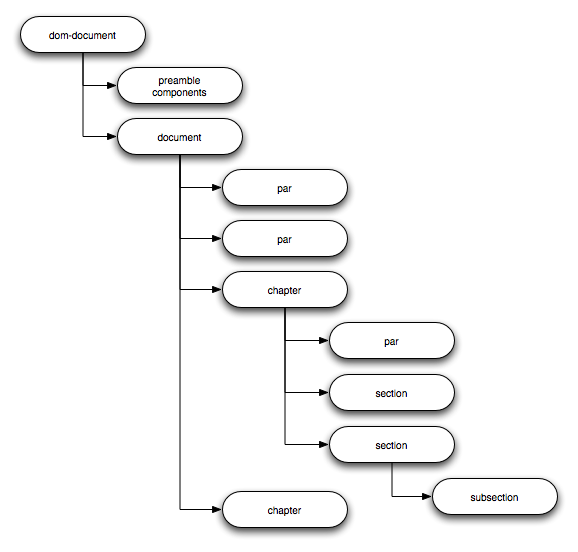
\includegraphics[width=4in]{docstructure}
\end{center}
\caption{The overall \plasTeX\ document structure\label{fig:docstructure}}
\end{figure}

This document is constructed during the parsing process by calling the 
\method{digest} method on each node.  The \method{digest} method is passed
an iterator of document nodes that correspond to the nodes in the document
that follow the current node.  It is the 
responsibility of the current node to only absorb the nodes that belong
to it during the digest process.  Luckily, the default \method{digest}
method will work in nearly all cases.  See section \ref{sec:macros} for more
information on the digestion process.

Part of this digestion process is grouping nodes into paragraphs.  This
is done using the \method{paragraphs} method available in all \class{Macro}
based classes.  This method uses the same technique as \TeX\ to group
paragraphs of content.  Section \ref{sec:paragraphs} has more information
about the details of paragraph grouping.

In addition to the \member{level} attribute of sections, there is also a
mixin class that assists in generating the table of contents and navigation
elements during rendering.  If you create your own sectioning commands,
you should include \class{plasTeX.Base.LaTeX.Sectioning.SectionUtils} as
a base class as well.  All of the standard \LaTeX\ section commands already
inherit from this class, so if you subclass one of those, you'll get
the helper methods for free.  For more information on these helper methods
see section \ref{sec:sections}.

The structure of the rest of the document is also fairly simple and 
well-defined.  \LaTeX\ commands are each converted into a document node
with it's arguments getting placed into the \member{attributes} dictionary.
\LaTeX\ environments also create a single node in the document, where
the child nodes of the environment include everything between the 
\macro{begin} and \macro{end} commands.  By default, the child nodes of
an environment are simply inserted in the order that they appear in the 
document.  However, there are some environments that require further
processing due to their more complex structures.  These structures include
arrays and tabular environments, as well as itemized lists.  For more
information on these structures see sections \ref{sec:arrays} and
\ref{sec:lists}, respectively.  Figures \ref{fig:docfragcode} and 
\ref{fig:docfrag} shows a common \LaTeX\ document fragment and the 
resulting \plasTeX\ document node structure.

\begin{figure}[ht]
\begin{verbatim}
\begin{center}
Every \textbf{good} boy does \textit{fine}.
\end{center}
\end{verbatim}
\caption{Sample \LaTeX\ document fragment code\label{fig:docfragcode}}
\end{figure}

\begin{figure}[ht]
\begin{center}
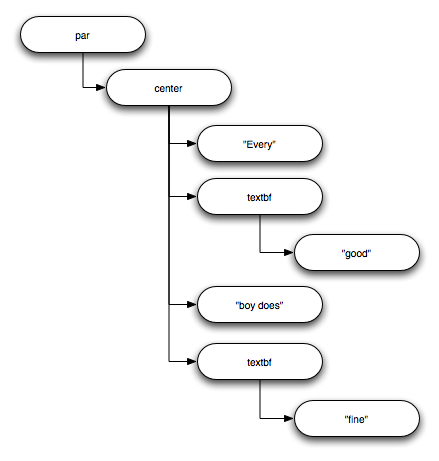
\includegraphics[width=3in]{docfrag}
\end{center}
\caption{Resulting \plasTeX\ document node structure\label{fig:docfrag}}
\end{figure}

You may have noticed that in the document structure in Figure \ref{fig:docfrag}
the text corresponding to the argument for \macro{textbf} and \macro{textit} 
is actually a child node and not an attribute.  This is actually a 
convenience feature in \plasTeX.  For macros like this where there is only
one argument and that argument corresponds to the content of the macro,
it is common to put that content into the child nodes.  This is done in
the \member{args} attribute of the macro class by setting the argument's
name to ``self''.  This magical value will link the attribute called 
``self'' to the child nodes array.  For more information on the \member{args}
attribute and how it populates the \member{attributes} dictionary see
section \ref{sec:macros}.

In the \plasTeX\ framework, the input \LaTeX\ document is parsed and 
digested until the document is finished.  At this point, you should have
an output document that conforms to the rules described above.  The 
document should have a regular enough structure that working with it
programatically using DOM methods or Python practices should be fairly
straight-forward.  The following sections give more detail on document
structure elements that require extra processing beyond the standard
parse-digest process.


\section{Sections\label{sec:sections}}

``Sections'' in \plasTeX\ refer to any macro that creates a section-like
construct in a document including the \environment{document} environment,
\macro{part}, \macro{chapter}, \macro{section}, \macro{subsection}, 
\macro{subsubsection}, \macro{paragraph}, and \macro{subparagraph}.
While these are the sectioning macros defined by \LaTeX, you are not limited
to using just those commands to create sections in your own documents.
There are two elements that must exist for a Python macro class to act
like a section: 1) the \member{level} attribute must be set to a value
less than 100, and 2) the class should inherit from 
\class{plasTeX.Base.LaTeX.Sectioning.SectionUtils}.

The \member{level} attribute refers to the section level in the document.
The values for this attribute are the same values that \LaTeX\ uses
for its section levels, namely:
\begin{description}
\item[-1 {\it or} \member{Node.PART_LEVEL}] corresponds to \macro{part}
\item[0 {\it or} \member{Node.CHAPTER_LEVEL}] corresponds to \macro{chapter}
\item[1 {\it or} \member{Node.SECTION_LEVEL}] corresponds to \macro{section}
\item[2 {\it or} \member{Node.SUBSECTION_LEVEL}] corresponds to \macro{subsection}
\item[3 {\it or} \member{Node.SUBSUBSECTION_LEVEL}] corresponds to \macro{subsubsection}
\item[4 {\it or} \member{Node.PARAGRAPH_LEVEL}] corresponds to \macro{paragraph}
\item[5 {\it or} \member{Node.SUBPARAGRAPH_LEVEL}] corresponds to \macro{subparagraph}
\end{description}

\plasTeX\ adds the following section related levels:
\begin{description}
\item[-\code{sys.maxint} {\it or} \member{Node.DOCUMENT_LEVEL}] 
    corresponds to the \environment{document} environment and 
    is always the top-level section
\item[6 {\it or} \member{Node.SUBSUBPARAGRAPH_LEVEL}]
    this level was added to correspond to the sixth level of headings
    defined in HTML
\item[100 {\it or} \member{Node.ENDSECTIONS_LEVEL}]
    flag that indicates the last possible section nesting level.  This is 
    mainly used for internal purposes.
\end{description}

\plasTeX\ uses the \member{level} attribute to build the appropriate 
document structure.  If all you need is a proper document structure,
the \member{level} attribute is the only thing that needs to be set on
a macro.  However, there are many convenience properties in the 
\class{plasTeX.Base.LaTeX.Sectioning.SectionUtils} class that are used
in the rendering process.  
If you plan on rendering your document, your
section classes should inherit from this class.  Below is a list
of the additional properties and their purpose.
\begin{tableii}{l|p{4in}}{member}{Name}{Purpose}
\lineii{allSections}{contains a sequential list of all of the sections 
    within and including the current section}
\lineii{documentSections}{contains a sequential list of all of the
    sections within the entire document}
\lineii{links}{contains a dictionary contain various amounts of 
    navigation information corresponding mostly to the link types 
    described at \url{http://fantasai.tripod.com/qref/Appendix/LinkTypes/ltdef.html}.
    This includes things like breadcrumb trails, previous and next links,
    links to the overall table of contents, etc.  See section \ref{sec:links}
    for more information.}
\lineii{siblings}{contains a list of all of the sibling sections}
\lineii{subsections}{contains a list of all of the sections within 
    the current section}
\lineii{tableofcontents}{contains an object that corresponds to the
    table of contents for the section.  The table of contents is 
    configurable as well.  For more information on how to configure
    the table of contents see section \ref{sec:tableofcontents}}
\end{tableii}
\note{When first accessed, each of these properties actually navigates the
      document and builds the returned object.  Since these operations
      can be rather costly, the values are cached.  Therefore, if you
      modify the document after accessing one of these properties you
      will not see the change reflected.}


\subsection{Navigation and Links\label{sec:links}}

The \class{plasTeX.Base.LaTeX.Sectioning.SectionUtils} class has a
property named \member{links} that contains a dictionary of many useful
objects that assist in creating navigation bars and breadcrumb trails
in the rendered output.  This dictionary was modeled after the links
described at \url{http://fantasai.tripod.com/qref/Appendix/LinkTypes/ltdef.html}.
Some of the objects in this dictionary are created automatically, others
are created with the help of the \member{linkType} attribute on the 
document nodes, and yet others can be added manually from a configuration
file or command-line options.  The automatically generated values are 
listed in the following table.
\begin{tableii}{l|p{4in}}{var}{Name}{Purpose}
\lineii{begin}{the first section of the document}
\lineii{breadcrumbs}{a list containing the entire parentage of the 
    current section (including the current section)}
\lineii{chapter}{the current chapter node}
\lineii{child}{a list of the subsections}
\lineii{contents}{the section that contains the top-level table of contents}
\lineii{document}{the document level node}
\lineii{end}{the last section of the document}
\lineii{first}{the first section of the document}
\lineii{home}{the first section of the document}
\lineii{home}{the first section of the document}
\lineii{last}{the last section of the document}
\lineii{navigator}{the section that contains the top-level table of contents}
\lineii{next}{the next section in the document}
\lineii{origin}{the section that contains the top-level table of contents}
\lineii{parent}{the parent node}
\lineii{part}{the current part node}
\lineii{prev}{the previous section in the document}
\lineii{previous}{the previous section in the document}
\lineii{section}{the current section}
\lineii{sibling}{a list of the section siblings}
\lineii{subsection}{the current subsection}
\lineii{start}{the first section of the document}
\lineii{toc}{the section that contains the top-level table of contents}
\lineii{top}{the first section of the document}
\lineii{up}{the parent section}
\end{tableii}
\note{The keys in every case are simply strings.}
\note{Each of the elements in the table above is either a section node or a list
of section nodes.  Of course, once you have a reference to a node you can
acces the attributes and methods of that object for further introspection.}
An example of accessing these objects from a section instance is shown below.
\begin{verbatim}
previousnode = sectionnode.links['prev']
nextnode = sectionnode.links['next']
\end{verbatim}

The next method of populating the links table is semi-automatic and uses
the \member{linkType} attribute on the Python macro class.  There are 
certain parts of a document that only occur once such as an index, 
glossary, or bibliography.  You can set the \member{linkType} attribute
on the Python macro class to a string that corresponds to that sections 
role in the document (i.e. `index' for the index, `glossary' for the glossary,
`bibliography' for the bibliography).  When a node with a special link
type is created, it is inserted into the dictionary of links with the 
given name.  This allows you to have links to indexes, glossaries, etc.
appear in the links object only when they are in the current document.
The example below shows the \environment{theindex} environment being
configured to show up under the `index' key in the links dictionary.
\begin{verbatim}
class theindex(Environment, SectionUtils):
    nodeType = 'index'
    level = Environment.SECTION_LEVEL
\end{verbatim}
\note{These links are actually stored under the `links' key of the
      owner document's userdata dictionary (i.e. 
      \code{self.ownerDocument.userdata['links'])}. Other objects can
      be added to this dictionary manually.}

The final way of getting objects into the links dictionary is through 
a configuration file or command-line options.  This method is described
fully in section \ref{sec:config-links}.


\subsection{Table of Contents\label{sec:tableofcontents}}

The table of contents object returned by the \member{tableofcontents}
property of \class{SectionUtils} is not an actual node of the document,
but it is a proxy object that limits the number of levels that you can
traverse.  The number of levels that you are allowed to traverse is
determined by \configkeys{document}{toc-depth} section of the configuration
(see section \ref{sec:config-document}).  Other than the fact that you
can only see a certain number of levels of subsections, the object 
otherwise acts just like any other section node.

In addition to limiting the number of levels of a table of contents,
you can also determine whether or not sections that do not generate new
files while rendering should appear in the table of contents.  By
default, only sections that generate a new file while rendering will
appear in the table of contents object.  If you set the value of
\configkeys{document}{toc-non-files} in the configuration to \code{True},
then all sections will appear in the table of contents.


\section{Paragraphs\label{sec:paragraphs}}

Paragraphs in a \plasTeX\ document are grouped in the same way that they
are grouped in \TeX: essentially anything within a section that isn't a
section itself is put into a paragraph.  This is different than the HTML
model where tables and lists are not grouped into paragraphs.  Because
of this, it is likely that HTML generated that keeps the same paragraph
model will not be 100\% valid.  However, it is highly unlikely that this 
variance from validity will cause any real problems in the browser 
rendering the correct output.

Paragraphs are grouped using the \method{paragraphs} method available on
all Python macro classes.  When this method is invoked on a node, 
all of the child nodes are grouped into paragraphs.  If there are no
paragraph objects in the list of child nodes already, one is created.
This is done to make sure that the document is fully normalized and 
that paragraphs occur everywhere that they can occur.  This is
most noteworthy in constructs like tables and lists where some table cells
or list items have multiple paragraphs and others do not.  If a paragraph
weren't forced into these areas, you could have inconsistently 
paragraph-ed content.

Some areas where paragraphs are allowed, but not necessarily needed might
not want the forced paragraph to be generated, such as within a grouping
of curly braces (\{~\}).  In these cases, you can
use the \code{force=False} keyword argument to \method{paragraphs}.
This still does paragraph grouping, but only if there is a paragraph element
already in the list of child nodes.


\section{Complex Structures\label{sec:complexdoc}}

While much of a \plasTeX\ document mirrors the structure of the source
\LaTeX\ document, some constructs do require a little more work to be
useful in the more rigid structure.  The most noteworthy of these 
constructs are lists, arrays (or tabular environments), and indexes.  
These objects are described in more detail in the following sections.


\subsection{Lists\label{sec:lists}}

Lists are normalized slightly more than the rest of the document.
They are treated almost like sections in that they are only allowed to
contain a minimal set of child node types.  In fact, lists can only
contain one type of child node: list item.  The consequence of this is that
any content before the first item in a list will be thrown out.  In turn, 
list items will only contain paragraph nodes.  The structure of all
list structures will look like the structure in Figure \ref{fig:liststruct}.

\begin{figure}[ht]
\begin{center}
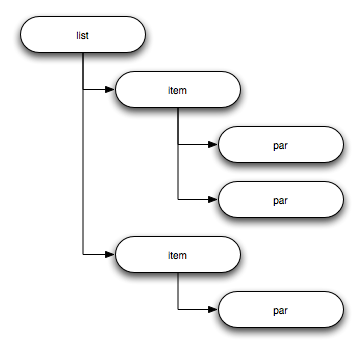
\includegraphics[width=3in]{liststruct}
\end{center}
\caption{Normalized structure of all lists\label{fig:liststruct}}
\end{figure}

This structure allows you to easily traverse a list with code like the
following.
\begin{verbatim}
# Iterate through the items in the list node
for item in listnode:

    # Iterate through the paragraphs in each item
    for par in item:

        # Print the text content of each paragraph
        print par.textContent

    # Print a blank line to separate each item
    print
\end{verbatim}

\subsection{Bibliography}

The bibliography is really just another list structure with a few 
enhancements to allow referencing of the items throughout the document.
Bibliography processing is left to the normal tools.  \plasTeX\
expects a properly \file{.bbl} file for the bibliography.  
The \LaTeX\ bibliography is the format used by default; however, 
the natbib package is also included with \plasTeX\ for more 
complex formatting of bibliographies.


\subsection{Arrays and Tabular Environments\label{sec:arrays}}

Arrays and tabular environments are the most complex structures in a 
\plasTeX\ document.  This because tables can include spanning columns,
spanning rows, and borders specified on the table, rows, and individual 
cells.  In addition, there are alignments associated with each column
and alignments can be specified by any \macro{multicolumn} command.
It is also possible with some packages to create your own column 
declarations.  Add to that the fact that the longtable package allows
you to specify multiple headers, footers, and coptions, and you can see
why tabular environments can be rather tricky to deal with.

As with all parts of the document, \plasTeX\ tries to normalize all tables
to have a consistent structure.  The structure for arrays and tables is 
shown in Figure \ref{fig:tablestruct}.
\begin{figure}[ht]
\begin{center}
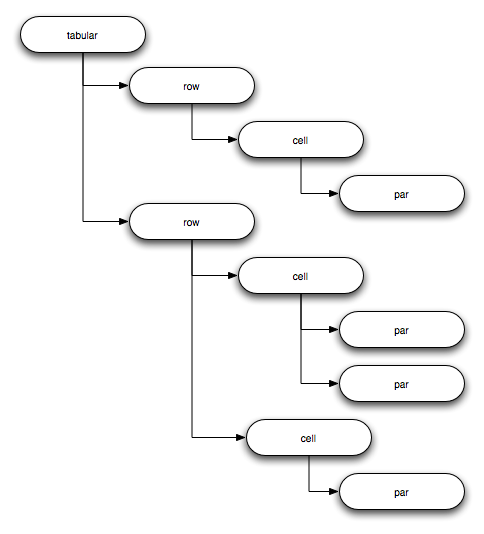
\includegraphics[width=4in]{tablestruct}
\end{center}
\caption{Normalized structure of all tables and arrays\label{fig:tablestruct}}
\end{figure}

Luckily, the array macro class that comes with \plasTeX\ was made to handle
all of the work for you.  In fact, it also handles the work of some extra 
packages such as longtable to make processing them transparent. The details
of the tabular environments are described in the following sections.

With this normalized structure, you can traverse all array and table 
structures with code like the following.
\begin{verbatim}
# Iterate through all rows in the table
for row in tablenode:

    # Iterate through all cells in the row
    for cell in row:

        # Iterate through all paragraphs in the cell
        for par in cell:

            # Print the text content of each cell
            print '   ' + par.textContent 

        # Print a blank line after each cell
        print

    # Print a blank line after each row
    print
\end{verbatim}


\subsubsection{Borders}

Borders in a tabular environment are generally handled by \macro{hline},
\macro{vline}, \macro{cline}, as well as the column specifications on 
the tabular environment and the \macro{multicolumn} command.  
\plasTeX\ merges all of the border specifications and puts them into 
CSS formatted values in the \member{style} attribute of each of the 
table cell nodes.  To get the CSS information formatted such that it
can be used in an inline style, simply access the \member{inline} property
of the style object. 

Here is an example of a \environment{tabular} environment.
\begin{verbatim}
\begin{tabular}{|l|l|}\hline
x & y \\
1 & 2 \\\hline
\end{tabular}
\end{verbatim}

The table node can be traversed as follows.
\begin{verbatim}
# Print the CSS for the borders of each cell
for rownum, row in enumerate(table):
    for cellnum, cell in enumerate(row):
        print '(%s,%s) %s -- %s' % (rownum, cellnum, 
               cell.textContent.strip(), cell.style.inline)
\end{verbatim}

The code above will print the following output (whitespace has been added
to make the output easier to read).
\begin{verbatim}
(0,0) x -- border-top-style:solid; 
           border-left:1px solid black; 
           border-right:1px solid black; 
           border-top-color:black; 
           border-top-width:1px; 
           text-align:left
(0,1) y -- border-top-style:solid; 
           text-align:left; 
           border-top-color:black; 
           border-top-width:1px; 
           border-right:1px solid black
(1,0) 1 -- border-bottom-style:solid; 
           border-bottom-width:1px; 
           border-left:1px solid black; 
           border-right:1px solid black; 
           text-align:left; 
           border-bottom-color:black
(1,1) 2 -- border-bottom-color:black; 
           border-bottom-width:1px; 
           text-align:left; 
           border-bottom-style:solid; 
           border-right:1px solid black
\end{verbatim}


\subsubsection{Alignments}

Alignments can be specified in the column specification of the tabular 
environment as well as in the column specification of \macro{multicolumn}
commands.  Just like the border information, the alignment information
is also stored in CSS formatted values in each cell's \member{style}
attribute.


\subsubsection{Longtables}

Longtables are treated just like regular tables.  Only the first header
and the last footer are supported in the resulting table structure.
To indicate that these are verifiable header or footer cells, the 
\member{isHeader} attribute of the corresponding cells is set to 
\code{True}.  This information can be used by the renderer to more 
accurately represent the table cells.


\subsection{Indexes}

All index building and sorting is done internally in \plasTeX.  It is 
done this way because the information that tools like \program{makeindex}
generate is only useful to \LaTeX\ itself since the refence to the 
place where the index tag was inserted is simply a page number.  Since
\plasTeX\ wants to be able to reference the index tag node, it has 
to do all of the index processing natively.

There are actually two index structures.  The default structure is simply 
the index nodes sorted and grouped into the appropriate hierarchies.
This structure looks like the structure pictured in Figure 
\ref{fig:defaultindex}.
\begin{figure}[ht]
\begin{center}
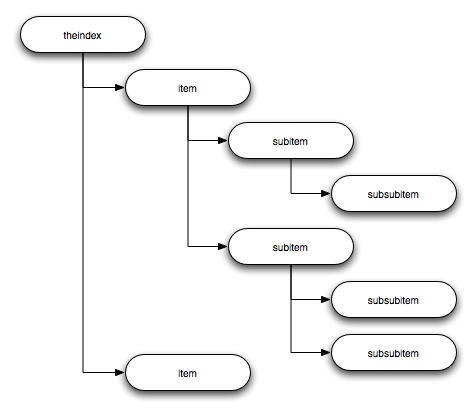
\includegraphics[width=4in]{defaultindex}
\end{center}
\caption{Default index structure\label{fig:defaultindex}}
\end{figure}

Each item, subitem, and subsubitem has an attribute called \member{key}
that contains a document fragment of the key for that index item.
The document nodes that this key corresponds to are held in a list
in the \member{pages} attribute.  These nodes are the actual 
nodes corresponding to the index entry macros from the \LaTeX\ document.
The content of the node is a number corresponding to the index entry
that is formatted according to the formatting rules specified in the
index entry.

While the structure above works well for paged media, it is sometimes 
nice to have the index entries grouped by first letter and possibly
even arranged into multiple columns.  This alternate representation
can be accessed in the \member{groups} property.  The structure 
for this type of index is shown in Figure \ref{fig:groupedindex}.
\begin{figure}[ht]
\begin{center}
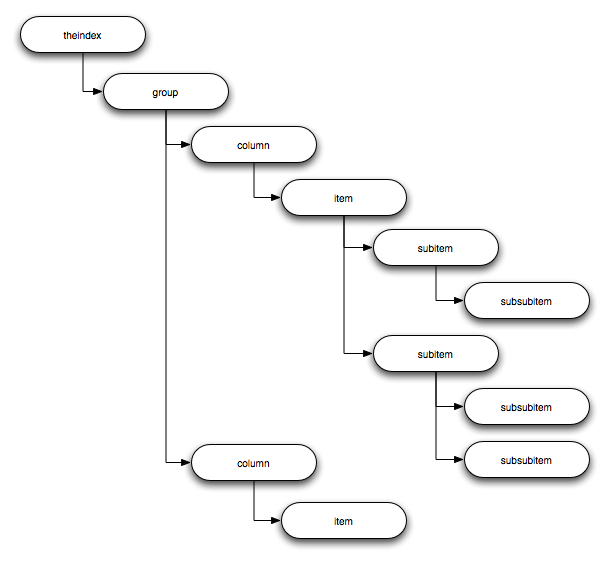
\includegraphics[width=4in]{groupedindex}
\end{center}
\caption{Grouped index structure\label{fig:groupedindex}}
\end{figure}

In this case, the item, subitem, and subsubitem nodes are the same as in
the default scheme.  The group has a \member{title} attribute that contains
the first letter of the entries in that group.  Entries that start with
something other than a letter or an underscore are put into a group
called ``Symbols''.  The columns are approximately equally sized columns
of index entries.  The number of columns is determined by the 
\configkeys{document}{index-columns} configuration item.



\chapter{Understanding Macros and Packages\label{sec:macros}}

Macros and packages in \plasTeX\ live a dual life.  On one hand, macros
can be defined in \LaTeX\ files and expanded by \plasTeX\ itself.  On
the other hand, macros can also be implemented as Python classes.
Packages are the same way.  \plasTeX\ can handle some \LaTeX\ packages
natively.  Others may have to be implemented in Python.  In most
cases, both implementations work transparently together.  If you don't
define that many macros, and the ones that you do define are simple
or even of intermediate complexity, it's probably better to just let
\plasTeX\ handle them natively. However, 
there are some reasons that you may want to implement Python versions
of your macros:
\begin{itemize}
\item Python versions of macros are generally faster
\item You have more control over what gets inserted into the output document
\item You can store information in the document's \member{userdata}
    dictionary for use later 
\item You can prevent a macro from being expanded into primitive \LaTeX\
    commands, so that a custom renderer can be used on that node
\item Some macros just don't make sense in a \plasTeX\ document
\item Some macros are just too complicated for \plasTeX
\end{itemize}

If any of these reasons appeal to you, read the following sections on
how to implement macros and packages in \plasTeX.


\section{Defining Macros in \LaTeX}

Defining macros in \LaTeX\ using \plasTeX\ is no different than the way
you would normally define you macros; however, there is a trick that you
can use to improve you macros for \plasTeX, if needed.  While \plasTeX\
can handle fairly complicated macros, some macros might do things that
don't make sense in the context of a \plasTeX\ document, or they might
just be too complicated for the \plasTeX\ engine to handle.  In
cases such as these, you can use the \macro{ifplastex} construct.
As you may know in \TeX, you can define your own \macro{if} commands using
the \macro{newif} primitive.  There is an \macro{if} command called
\macro{ifplastex} built into the \plasTeX\ engine that is always set to
true.  In you document, you can define this command and set it to 
false (as far as \LaTeX\ is concerned) as follows.
\begin{verbatim}
\newif\ifplastex
\plastexfalse
\end{verbatim}

Now you can surround the portions of your macros that \plasTeX\ has 
trouble with, or even write alternative versions of the macro for 
\LaTeX\ and \plasTeX.  Here is an example.
\begin{verbatim}
\newcommand{\foo}[1]{
    \ifplastex\else\vspace*{0.25in}\fi
    \textbf{\Large{#1}}
    \ifplastex\else\vspace*{1in}\fi
}

\ifplastex
    \newenvironment{coolbox}{}{}
\else
    \newenvironment{coolbox}
        {fbox\bgroup\begin{minipage}{5in}}
        {\end{minipage}\egroup}
\fi
\end{verbatim}


\section{Defining Macros in Python}

Defining macros using Python classes (or, at least through Python interfaces)
is done in one of three ways: INI files, Python classes, and the document
context.  These three methods are described in the following sections.


\subsection{Python Classes\label{sec:macroclasses}}

Both \LaTeX\ command and environments can be implemented in Python
classes.  \plasTeX\ includes a base class for each one: \class{Command}
for commands and \class{Environment} for environments.  For the most
part, these two classes behave in the same way.  They both are 
responsible for parsing their arguments, organizing their child nodes,
incrementing counters, etc. much like their \LaTeX\ counterparts.
There is also a variant of the \class{Environment} class called 
\class{NoCharSubEnvironment} which temporarily turns off character
substitutions described in Section~\ref{sec:texdocument-objects}.
The Python macro class feature set is based on common \LaTeX\ 
conventions.  So if the \LaTeX\ macro you are implementing in Python
uses standard \LaTeX\ conventions, you job will be very easy.  If you
are doing unconventional operations, you will probably still succeed,
you just might have to do a little more work.

The three most important parts of the Python macro API are: 1) the 
\member{args} attribute, 2) the \method{invoke} method, and 3) the
\member{digest} method.  When writing your own macros, these are
used the most by far.

\subsubsection{The \member{args} Attribute}

The \member{args} attribute is a string attribute on the class 
that indicates what the arguments to the macro are.  In addition to
simply indicating the number of arguments, whether they are mandatory
or optional, and what characters surround the argument as in \LaTeX,
the \member{args} string also gives names to each of the argument
and can also indicate the content of the argument (i.e. int, float,
list, dictionary, string, etc.).  The names given to each argument
determine the key that the argument is stored under in the the
\member{attributes} dictionary of the class instance.  Below is a simple
example of a macro class.
\begin{verbatim}
from plasTeX import Command, Environment

class framebox(Command):
    """ \framebox[width][pos]{text} """
    args = '[ width ] [ pos ] text'
\end{verbatim}

In the \member{args} string of the \macro{framebox} macro, three arguments
are defined.  The first two are optional and the third one is mandatory.
Once each argument is parsed, in is put into the \member{attributes}
dictionary under the name given in the \member{args} string.  For example,
the \member{attributes} dictionary of an instance of \macro{framebox}
will have the keys ``width'', ``pos'', and ``text'' once it is parsed
and can be accessed in the usual Python way.
\begin{verbatim}
self.attributes['width']
self.attributes['pos']
self.attributes['text']
\end{verbatim}

In \plasTeX, any argument that isn't mandatory (i.e. no grouping characters
in the \member{args} string) is optional\footnote{While this isn't always true
when \LaTeX\ expands the macros, it will not cause any problems when
\plasTeX\ compiles the document because \plasTeX\ is less stringent.}.
This includes arguments surrounded by parentheses ((~)), square brackets
([~]), and angle brackets (<~>).  This also lets you combine multiple
versions of a command into one macro.  For example, the \macro{framebox}
command also has a form that looks like: 
\macro{framebox(x_dimen,y_dimen)[pos]\{text\}}.  This leads to the 
Python macro class in the following code sample that encompasses both 
forms.
\begin{verbatim}
from plasTeX import Command, Environment

class framebox(Command):
    """ 

    \framebox[width][pos]{text} or 
    \framebox(x_dimen,ydimen)[pos]{text} 

    """
    args = '( dimens ) [ width ] [ pos ] text'
\end{verbatim}
The only thing to keep in mind is that in the second form, the \var{pos}
attribute is going to end up under the \var{width} key in the 
\member{attributes} dictionary since it is the first argument in 
square brackets, but this can be fixed up in the \method{invoke} method
if needed.  Also, if an optional argument is not present on the 
macro, the value of that argument in the \member{attributes} dictionary
is set to \var{None}.

As mentioned earlier, it is also possible to convert arguments
to data types other than the default (a document fragment).  A list
of the available types is shown in the table below.
\begin{tableii}{l|p{4in}}{var}{Name}{Purpose}
\lineii{str}{expands all macros then sets the value of the argument
   in the \member{attributes} dictionary to the string content of the argument}
\lineii{chr}{same as `str'}
\lineii{char}{same as `str'}
\lineii{cs}{sets the attribute to an unexpanded control sequence}
\lineii{label}{expands all macros, converts the result to a string, then sets
    the current label to the object that is in the \member{currentlabel}
    attribute of the document context.  Generally, an object is put into the 
    \member{currentlabel} attribute if it incremented a counter when it
    was invoked.  The value stored in the \member{attributes} dictionary
    is the string value of the argument.}
\lineii{id}{same as `label'}
\lineii{idref}{expands all macros, converts the result to a string, 
    retrieves the object that was labeled by that value,
    then adds the labeled object to the \member{idref} dictionary under
    the name of the argument.
    This type of argument is used in commands like \macro{ref} that must
    reference other abjects.  The nice thing about `idref' is that it
    gives you a reference to the object itself which you can then use
    to retrieve any type of information from it such as the reference
    value, title, etc.  The value stored in the \member{attributes} 
    dictionary is the string value of the argument.}
\lineii{ref}{same as `idref'}
\lineii{nox}{just parses the argument, but doesn't expand the macros}
\lineii{list}{converts the argument to a Python list.  By default, the list item
    separator is a comma (,).  You can change the item separator in
    the args string by appending a set of parentheses surrounding the 
    separator character immediately after `list'.  For example, to
    specify a semi-colon separated list for an argument called ``foo''
    you would use the \member{args} string: ``foo:list(;)''.  It is also
    possible to cast the type of each item by appending another colon
    and the data type from this table that you want each item to be.
    However, you are limited to one data type for every item in the list.}
\lineii{dict}{converts the argument to a Python dictionary.  This is commonly
    used by arguments set up using \LaTeX's \file{keyval} package.
    By default, key/value pairs are separated by commas, although this
    character can be changed in the same way as the delimiter in the
    `list' type.  You can also cast each value of the dictionary using
    the same method as the `list' type.  In all cases, keys are converted
    to strings.}
\lineii{dimen}{reads a dimension and returns an instance of \class{dimen}}
\lineii{dimension}{same as `dimen'}
\lineii{length}{same as `dimen'}
\lineii{number}{reads an integer and returns a Python integer}
\lineii{count}{same as `number'}
\lineii{int}{same as `number'}
\lineii{float}{reads a decimal value and returns a Python float}
\lineii{double}{same as `float'}
\end{tableii}

There are also several argument types used for more low-level routines.
These don't parse the typical \LaTeX\ arguments, they are used for
the somewhat more free-form \TeX\ arguments.
\begin{tableii}{l|p{4in}}{var}{Name}{Purpose}
\lineii{Dimen}{reads a \TeX\ dimension and returns an instance of \class{dimen}}
\lineii{Length}{same as `Dimen'}
\lineii{Dimension}{same as `Dimen'}
\lineii{MuDimen}{reads a \TeX\ mu-dimension and returns an instance of \class{mudimen}}
\lineii{MuLength}{same as `MuDimen'}
\lineii{Glue}{reads a \TeX\ glue parameter and returns an instance of \class{glue}}
\lineii{Skip}{same as `MuLength'}
\lineii{Number}{reads a \TeX\ integer parameter and returns a Python integer}
\lineii{Int}{same as `Number'}
\lineii{Integer}{same as `Number'}
\lineii{Token}{reads an unexpanded token}
\lineii{Tok}{same as `Token'}
\lineii{XToken}{reads an expanded token}
\lineii{XTok}{same as `XToken'}
\lineii{Args}{reads tokens up to the first begin group (i.e. \{)}
\end{tableii}

To use one of the data types, simple append a colon (:) and the data
type name to the attribute name in the \member{args} string.
Going back to the \macro{framebox} example, the argument in 
parentheses would be better represented as a list of dimensions.
The \var{width} parameter is also a dimension, and the \var{pos} parameter
is a string.
\begin{verbatim}
from plasTeX import Command, Environment

class framebox(Command):
    """ 

    \framebox[width][pos]{text} or 
    \framebox(x_dimen,ydimen)[pos]{text} 

    """
    args = '( dimens:list:dimen ) [ width:dimen ] [ pos:chr ] text'
\end{verbatim}


\subsubsection{The \method{invoke} Method}

The \method{invoke} method is responsible for creating a new document
context, parsing the macro arguments, and incrementing counters.
In most cases, the default implementation will work just fine, but you
may want to do some extra processing of the macro arguments or 
counters before letting the parsing of the document proceed.  There
are actually several methods in the API that are called within the
scope of the \method{invoke} method: \method{preParse}, \method{preArgument},
\method{postArgument}, and \method{postParse}.

The order of execution is quite simple.  Before any arguments have been
parsed, the \method{preParse} method is called.  The \method{preArgument}
and \method{postArgument} methods are called before and after each
argument, respectively.  Then, after all arguments have been parsed, the
\method{postParse} method is called.  The default implementations of 
these methods handle the stepping of counters and setting the 
current labeled item in the document.  By default, macros that have
been ``starred'' (i.e. have a `*' before the arguments) do not 
increment the counter.  You can override this behavior in one of these
methods if you prefer.

The most common reason for overriding the \method{invoke} method is to
post-process the arguments in the \member{attributes} dictionary, or
add information to the instance.
For example, the \macro{color} command in \LaTeX's color package
could convert the \LaTeX\ color to the correct CSS format
and add it to the CSS style object.
\begin{verbatim}
from plasTeX import Command, Environment

def latex2htmlcolor(arg):
    if ',' in arg:
        red, green, blue = [float(x) for x in arg.split(',')]
        red = min(int(red * 255), 255)
        green = min(int(green * 255), 255)
        blue = min(int(blue * 255), 255)
    else:
        try:
            red = green = blue = float(arg)
        except ValueError:
            return arg.strip()
    return '#%.2X%.2X%.2X' % (red, green, blue)

class color(Environment):
    args = 'color:str'
    def invoke(self, tex):
        a = Environment.invoke(tex)
        self.style['color'] = latex2htmlcolor(a['color'])
\end{verbatim}

While simple things like attribute post-processing is the most common
use of the \method{invoke} method, you can do very advanced things
like changing category codes, and iterating over the tokens in the
\TeX\ processor directly like the \environment{verbatim} environment
does.

One other feature of the \method{invoke} method that may be of interest
is the return value.  Most \method{invoke} method implementations do
not return anything (or return \var{None}).  In this case, the macro
instance itself is sent to the output stream.  However, you can also
return a list of tokens.  If a list of tokens is returned, instead of
the macro instance, those tokens are inserted into the output stream.
This is useful if you don't want the macro instance to be part of the
output stream or document.  In this case, you can simply return an
empty list.


\subsubsection{The \method{digest} Method}

The \method{digest} method is responsible for converting the output
stream into the final document structure.  For commands, this generally
doesn't mean anything since they just consist of arguments which 
have already been parsed.  Environments, on the other hand, have a 
beginning and an ending which surround tokens that belong to that
environment.  In most cases, the tokens between the \macro{begin}
and \macro{end} need to be absorbed into the \member{childNodes}
list.

The default implementation of the \method{digest} method should work
for most macros, but there are instances where you may want to 
do some extra processing on the document structure.  For example,
the \macro{caption} command within \environment{figure}s and 
\environment{table}s uses the \method{digest} method to populate
the enclosing figure/table's \method{caption} attribute.
\begin{verbatim}
from plasTeX import Command, Environment

class Caption(Command):
    args = '[ toc ] self'

    def digest(self, tokens):
        res = Command.digest(self, tokens)

        # Look for the figure environment that we belong to 
        node = self.parentNode
        while node is not None and not isinstance(node, figure):
            node = node.parentNode

        # If the figure was found, populate the caption attribute
        if isinstance(node, figure):
            node.caption = self

        return res

class figure(Environment):
    args = '[ loc:str ]'
    caption = None
    class caption_(Caption):
        macroName = 'caption'
        counter = 'figure'
\end{verbatim}

More advanced uses of the \method{digest} method might be to construct
more complex document structures.  For example, tabular and array
structures in a document get converted from a simple list of tokens
to complex structures with lots of style information added (see section
\ref{sec:arrays}).  One simple example of a \method{digest} that 
does something extra is shown below.  It looks for the first 
node with the name ``item'' then bails out.
\begin{verbatim}
from plasTeX import Command, Environment

class toitem(Command):
    def digest(self, tokens):
        """ Throw away everything up to the first 'item' token """
        for tok in tokens:
            if tok.nodeName == 'item':
               # Put the item back into the stream
               tokens.push(tok)
               break
\end{verbatim}

One of the more advanced uses of the \method{digest} is on the sectioning
commands: \macro{section}, \macro{subsection}, etc.  The digest method
on sections absorb tokens based on the \member{level} attribute which
indicates the hierarchical level of the node.  When digested, each section
absorbs all tokens until it reaches a section that has a level that is
equal to or higher than its own level.  This creates the overall 
document structure as discussed in section \ref{sec:document}.


\subsubsection{Other Nifty Methods and Attributes}

There are many other attributes and methods on macros that can be used
to affect their behavior.  For a full listing, see the API documentation
in section \ref{sec:macros-api}.  Below are descriptions of some of the
more commonly used attributes and methods.

\paragraph{The \member{level} attribute}
The \member{level} attribute is an integer that indicates the 
hierarchical level of the node in the output document structure.  
The values of this attribute are taken from \LaTeX: \macro{part}
is -1, \macro{chapter} is 0, \macro{section} is 1, \macro{subsection}
is 2, etc.  To create your owne sectioning commands, you can either
subclass one of the existing sectioning macros, or simply set its
\member{level} attribute to the appropriate number.

\paragraph{The \member{macroName} attribute}
The \member{macroName} attribute is used when you are creating a
\LaTeX\ macro whose name is not a legal Python class name.  
For example, the macro \macro{@ifundefined} has a `@' in the name
which isn't legal in a Python class name.  In this case, you could define
the macro as shown below.
\begin{verbatim}
class ifundefined_(Command):
    macroName = '@ifundefined'
\end{verbatim}

\paragraph{The \member{counter} attribute}
The \member{counter} attribute associates a counter with the macro
class.  It is simply a string that contains the name of the counter.
Each time that an instance of the macro class is invoked, the
counter is incremented (unless the macro has a `*' argument).

\paragraph{The \member{ref} attribute}
The \member{ref} attribute contains the value normally returned
by the \macro{ref} command.

\paragraph{The \member{title} attribute}
The \member{title} attribute retrieves the ``title'' attribute from
the \member{attributes} dictionary.  This attribute is also overridable.

\paragraph{The \member{fullTitle} attribute}
The same as the \member{title} attribute, but also includes the 
counter value at the beginning.

\paragraph{The \member{tocEntry} attribute}
The \member{tocEntry} attribute retrieves the ``toc'' attribute from
the \member{attributes} dictionary.  This attribute is also overridable.

\paragraph{The \member{fullTocEntry} attribute}
The same as the \member{tocEntry} attribute, but also includes the 
counter value at the beginning.

\paragraph{The \member{style} attribute}
The \member{style} attribute is a CSS style object.  Essentially, this is
just a dictionary where the key is the CSS property name and the value 
is the CSS property value.  It has an attribute called \member{inline}
which contains an inline version of the CSS properties for use
in the style= attribute of HTML elements.

\paragraph{The \member{id} attribute}
This attribute contains a unique ID for the object.  If the object
was labeled by a \macro{label} command, the ID for the object will 
be that label; otherwise, an ID is generated.

\paragraph{The \member{source} attribute}
The \member{source} attribute contains the \LaTeX\ source representation
of the node and all of its contents.

\paragraph{The \method{currentSection} attribute}
The \member{currentSection} attribute contains the section that the
node belongs to.

\paragraph{The \method{expand} method}
The \method{expand} method is a thin wrapper around the \method{invoke}
method.  It simply invokes the macro and returns the result of 
expanding all of the tokens.  Unlike \method{invoke}, you will 
always get the expanded node (or nodes); you will not get a \var{None}
return value.

\paragraph{The \method{paragraphs} method}
The \method{paragraphs} method does the final processing of paragraphs
in a node's child nodes.  It makes sure that all content is wrapped
within paragraph nodes.  This method is generally called from the
\method{digest} method.


\subsection{INI Files\label{sec:inimacros}}

Using INI files is the simplest way of creating customized Python macro
classes.  It does require a little bit of knowledge of writing 
macros in Python classes (section \ref{sec:macroclasses}), but not 
much.  The only two pieces of information about Python macro classes
you need to know are 1) the \member{args} string format, and 2)
the superclass name (in most cases, you can simply use \class{Command}
or \class{Environment}).  The INI file features correspond to Python
macros in the following way.
\begin{tableii}{l|l}{}{INI File}{Python Macro Use}
\lineii{section name}{the Python class to inherit from}
\lineii{option name}{the name of the macro to create}
\lineii{option value}{the args string for the macro}
\end{tableii}

Here is an example of an INI file that defines several macros.
\begin{verbatim}
[Command]
; \program{ self }
program=self
; \programopt{ self }
programopt=self

[Environment]
; \begin{methoddesc}[ classname ]{ name  { args } ... \end{methoddesc}
methoddesc=[ classname ] name args
; \begin{memberdesc}[ classname ]{ name  { args } ... \end{memberdesc}
memberdesc=[ classname ] name args

[section]
; \headi( options:dict )[ toc ]{ title }
headi=( options:dict ) [ toc ] title

[subsection]
; \headii( options:dict )[ toc ]{ title }
headii=( options:dict ) [ toc ] title
\end{verbatim}

In the INI file above, six macro are being defined.  \macro{program} and
\macro{programopt} both inherit from \class{Command}, the generic 
\LaTeX\ macro superclass.  They also both take a single mandatory argument
called ``self.''  There are two environments defined also: 
\environment{methoddesc} and \environment{memberdesc}.  Each of these
has three arguments where the first argument is optional.  The 
last two macros actually inherit from standard \LaTeX\ sectioning commands.
They add an option, surrounded by parentheses, to the options that
\macro{section} and \macro{subsection} already had defined.

INI versions of \plasTeX\ packages are loaded much in the same way as
Python \plasTeX\ packages.  For details on how packages are loaded, see
section \ref{sec:packages}.


\subsection{The Document Context\label{sec:contextmacros}}

It is possible to define commands using the same interface that is used
by the \plasTeX\ engine itself.  This interface belongs to the 
\class{Context} object (usually accessed through the document object's
\member{context} attribute).  Defining commands using the context object
is generally done in the \function{ProcessOptions} function of a 
package.  The following methods of the context object create new commands.
\begin{tableii}{l|p{4in}}{method}{Method}{Purpose}
\lineii{newcounter}{creates a new counter, and also creates a command
    called \macro{the{\it counter}} which generates the formatted version
    of the counter.  This macro corresponds to the \macro{newcounter} 
    macro in \LaTeX.}
\lineii{newcount}{corresponds to \TeX's \macro{newcount} command.}
\lineii{newdimen}{corresponds to \TeX's \macro{newdimen} command.}
\lineii{newskip}{corresponds to \TeX's \macro{newskip} command.}
\lineii{newmuskip}{corresponds to \TeX's \macro{newmuskip} command.}
\lineii{newif}{corresponds to \TeX's \macro{newif} command.  This 
    command also generates macros for \macro{{\it ifcommand}true} and
    \macro{{\it ifcommand}false}.}
\lineii{newcommand}{corresponds to \LaTeX's \macro{newcommand} macro.}
\lineii{newenvironment}{corresponds to \LaTeX's \macro{newenvironment} macro.}
\lineii{newdef}{corresponds to \TeX's \macro{def} command.}
\lineii{chardef}{corresponds to \TeX's \macro{chardef} command.}
\end{tableii}

\note{Since many of these methods accept strings containing \LaTeX\ 
markup, you need to remember that the category codes of some characters
can be changed during processing.  If you are defining macros using
these methods in the \function{ProcessOptions} function in a package,
you should be safe since this function is executed in the preamble of the 
document where category codes are not changed frequently.  However, if
you define a macro with this interface in a context where the category
codes are not set to the default values, you will have to adjust the 
markup in your macros accordingly.}

Below is an example of using this interface within the context of a package
to define some commands.  For the full usage of these methods see the
API documentation of the \class{Context} object in section 
\ref{sec:context-api}.
\begin{verbatim}
def ProcessOptions(options, document):
    context = document.context

    # Create some counters
    context.newcounter('secnumdepth', initial=3)
    context.newcounter('tocdepth', initial=2)

    # \newcommand{\config}[2][general]{\textbf{#2:#1}
    context.newcommand('config', 2, r'\textbf{#2:#1}', opt='general')

    # \newenvironment{note}{\textbf{Note:}}{}
    context.newenvironment('note', 0, (r'\textbf{Note:}', r''))
\end{verbatim}


\section{Packages\label{sec:packages}}

Packages in \plasTeX\ are loaded in one of three ways: standard \LaTeX\
package, Python package, and INI file.  \LaTeX\ packages are loaded in
much the same way that \LaTeX\ itself loads packages.  The \program{kpsewhich}
program is used to locate the requested file which can be either in
the search path of your \LaTeX\ distribution or in one of the directories
specified in the \environment{TEXINPUTS} environment variable.
\plasTeX\ read the file and expand the macros therein just as \LaTeX\
would do.

Python packages are located using Python's search paths, listed in
\var{sys.path}. This includes the current directory as well as those listed in
the \environment{PYTHONPATH} environment variable. After a package is
loaded, it is checked to see if there is a function called
\function{ProcessOptions} in its namespace.  If there is, that function
is called with two arguments: 1) the dictionary of options that were
specified when loading the package, and 2) the document object that is
currently being processed.  This function allows you to make adjustments
to the loaded macros based on the options specified, and define new
commands in the document's context (see section \ref{sec:contextmacros} 
for more information).  Of course, you can also define Python based
macros (section \ref{sec:macroclasses}) in the Python package as well.

The last type of packages is based on the INI file format.  This 
format is discussed in more detail in section \ref{sec:inimacros}.
INI formatted packages are loaded in conjunction with a \LaTeX\ or
Python package.  When a package is loaded, an INI file with the same
basename is searched for in the same director as the package.  If it
exists, it is loaded as well.  For example, if you had a package
called \file{python.sty} and a file called \file{python.ini} in the same
package directory, \file{python.sty} would be loaded first,
then \file{python.ini} would be loaded.  The same operation applies 
for Python based packages.


\chapter{Renderers}

Renderers allow you to convert a \plasTeX\ document object into viewable
output such as HTML, RTF, or PDF, or simply a data structure format such
as DocBook or tBook.  Since the \plasTeX\ document object gives you
everything that you could possibly want to know about the \LaTeX\ document,
it should, in theory, be possible to generate any type of output from
the \plasTeX\ document object while preserving as much information as the
output format is capable of.  In addition, since the document object is
not affected by the rendering process, you can apply multiple renderers
in sequence so that the \LaTeX\ document only needs to be parsed one time
for all output types.

While it is possible to write a completely custom renderer, a couple of
renderer implementations are included with the \plasTeX\ framework.
While the rendering process in this implementation is fairly simple,
it is also very powerful.  Some of the main features are listed below.
\begin{itemize}
\item ability to generate multiple output files
\item automatic splitting of files is configurable by section level,
    or can be invoked using ad-hoc methods in the
    \member{filenameoverride} property
\item powerful output filename generation utility
\item image generation for portions of the document that cannot be
    easily rendered in a particular output formate (e.g. TikZ pictures in HTML)
\item themeing support
\item hooks for post-processing of output files
\item configurable output encodings
\end{itemize}

The API of the renderer itself is very small.  In fact, there are only
a couple of methods that are of real interest to an end user: \method{render}
and \method{cleanup}.  The \method{render} method is the method that starts
the rendering process.  It's only argument is a \plasTeX\ document object.
The \method{cleanup} method is called at the end of the rendering process.
It is passed the document object and a list of all of the files that were
generated.  This method allows you to do post-processing on the output files.
In general, this method will probably only be of interest to someone
writing a subclass of the \class{Renderer} class, so most users of
\plasTeX\ will only use the \method{render} method.  The real work of
the rendering process is handled in the \class{Renderable} class which
is discussed later in this chapter.

The \class{Renderer} class is a subclass of the Python dictionary.
Each key in the renderer corresponds to the name of a node in the
document object.  The value stored under each key is a function.
As each node in the document object is traversed, the renderer is queried
to see if there is a key that matches the name of the node.  If a
key is found, the value at that key (which must be a function) is
called with the node as its only argument.  The return value from this
call must be a string object that contains the rendered output.
Based on the configuration, the renderer will handle all of the file
generation and encoding issues.

If a node is traversed that doesn't correspond to a key in the
renderer dictionary, the default rendering method is called.  The
default rendering method is stored in the \member{default} attribute.
One exception to this rule is for text nodes.  The default
rendering method for text nodes is actually stored in \member{textDefault}.
Again, these attributes simply need to reference any Python function
that returns a string object of the rendered output.  The
default method in both of these attributes is the \function{str}
built-in function.

As mention previously, most of the work of the renderer is actually
done by the \class{Renderable} class.  This is a mixin class\footnote{
A mixin class is simply a class that is merely a collection of methods
that are intended to be included in the namespace of another class.} that is
mixed into the \class{Node} class in the \method{render} method.
It is unmixed at the end of the \method{render} method.  The details
of the \class{Renderable} class are discussed in section \ref{sec:renderable}.

\section{Simple Renderer Example}\label{sec:simple-renderer-ex}

It is possible to write a renderer with just a couple of methods:
\method{default} and \method{textDefault}.
The code below demonstrates how one might create a generic XML
renderer that simply uses the node names as XML tag names.
The text node renderer escapes the <, >, and \& characters.
\begin{verbatim}
import string
from plasTeX.Renderers import Renderer as _Renderer

class Renderer(_Renderer):

    def default(self, node):
        """ Rendering method for all non-text nodes """
        s = []

        # Handle characters like \&, \$, \%, etc.
        if len(node.nodeName) == 1 and node.nodeName not in string.ascii_letters:
            return self.textDefault(node.nodeName)

        # Start tag
        s.append('<%s>' % node.nodeName)

        # See if we have any attributes to render
        if node.hasAttributes():
            s.append('<attributes>')
            for key, value in node.attributes.items():
                # If the key is 'self', don't render it
                # these nodes are the same as the child nodes
                if key == 'self':
                    continue
                s.append('<%s>%s</%s>' % (key, str(value), key))
            s.append('</attributes>')

        # Invoke rendering on child nodes
        s.append(str(node))

        # End tag
        s.append('</%s>' % node.nodeName)

        return '\n'.join(s)

    def textDefault(self, node):
        """ Rendering method for all text nodes """
        return node.replace('&','&amp;').replace('<','&lt;').replace('>','&gt;')
\end{verbatim}

To use the renderer, simply parse a \LaTeX\ document and apply the renderer
using the \method{render} method.
\begin{verbatim}
# Import renderer from previous code sample
from MyRenderer import Renderer

from plasTeX.TeX import TeX

# Instantiate a TeX processor and parse the input text
tex = TeX()
tex.ownerDocument.config['files']['split-level'] = -100
tex.ownerDocument.config['files']['filename'] = 'test.xml'
tex.input(r'''
\documentclass{book}
\begin{document}

Previous paragraph.

\section{My Section}

\begin{center}
Centered text with <, >, and \& charaters.
\end{center}

Next paragraph.

\end{document}
''')
document = tex.parse()

# Render the document
renderer = Renderer()
renderer.render(document)
\end{verbatim}

The output from the renderer, located in \file{test.xml}, looks like the
following.
\begin{verbatim}
<document>
<par>
Previous paragraph.
</par><section>
    <attributes>
        <toc>None</toc>
        <*modifier*>None</*modifier*>
        <title>My Section</title>
    </attributes>
<par>
<center>
 Centered text with &lt;, &gt;, and &amp; charaters.
</center>
</par><par>
Next paragraph.
</par>
</section>
</document>
\end{verbatim}


\subsection{Extending the Simple Renderer}

Now that we have a simple renderer working, it is very simple to extend
it to do more specific operations.  Let's say that the default renderer
is fine for most nodes, but for the \macro{section} node we want to do
something special.  For the section node, we want the title argument
to correspond to the title attribute in the output XML\footnote{This
will only work properly in XML if the content of the title is plain text
since other nodes will generate markup.}.  To do this we need a
method like the following.
\begin{verbatim}
def handle_section(node):
    return '\n\n<%s title="%s">\n%s\n</%s>\n' % \
            (node.nodeName, str(node.attributes['title']),
             str(node), node.nodeName)
\end{verbatim}

Now we simply insert the rendering method into the renderer under the
appropriate key.  Remember that the key in the renderer should match
the name of the node you want to render.  Since the above rendering
method will work for all section types, we'll insert it into the
renderer for each \LaTeX\ sectioning command.
\begin{verbatim}
renderer = Renderer()
renderer['section'] = handle_section
renderer['subsection'] = handle_section
renderer['subsubsection'] = handle_section
renderer['paragraph'] = handle_section
renderer['subparagraph'] = handle_section
renderer.render(document)
\end{verbatim}

Running the same \LaTeX\ document as in the previous example, we now get
this output.
\begin{verbatim}
<document>
<par>
Previous paragraph.
</par>

<section title="My Section">
<par>
<center>
 Centered text with &lt;, &gt;, and &amp; charaters.
</center>
</par><par>
Next paragraph.
</par>
</section>

</document>
\end{verbatim}

Of course, you aren't limited to using just Python methods.  Any function
that accepts a node as an argument can be used.  The
Page Template renderer included with \plasTeX\ is an example
of how to write a renderer that uses a templating language to render
the nodes (see section \ref{sec:pt}).

\subsection{Using a Renderer from the plastex Script}
\label{subsec:renderer-from-script}

In the preceding sections, the simple renderer example was called from
a custom python script. In order to use it through the
main plastex script (described in Chapter~\ref{sec:command-line}), it
needs to be located in some directory
\verb+plasTeX/Renderers/SimpleRenderer+, where \verb+plasTeX+ is the
directory containing the plastex script. This directory must contain a
\verb+__init__.py+ file defining the \var{Renderer} class (with this
name). This directory can also contain a \verb+Themes+ directory in
order to use the theme option described in
Section~\ref{sec:general-options}. Each subdirectory in the
\verb+Themes+ directory is considered as a theme.

Each renderer can define its own configuration options which are loaded
by the plastex script. This is done in a file named \verb+Config.py+
in the renderer directory. This file must define a variable named
\var{config} which is a ConfigManager instance, as described in
Section~\ref{sec:configuration-api}. Inspiration can be drawn from the
file defining the global configuration which is
\verb+plasTeX/Config.py+.

For instance, one could add a file
\verb+plasTeX/Renderers/SimpleRenderer/Config.py+ containing:

\begin{verbatim}
from plasTeX.ConfigManager import *

config = ConfigManager()

section = config.add_section('simplerenderer')

config.add_category('simplerenderer', 'Simple Renderer Options')

section['my-option'] = StringOption(
    """ My option """,
    options='--my-option',
    category='simplerenderer',
    default='',
)
\end{verbatim}

Options values are attached to the document currently rendered. For
instance, in the \var{default} method implemented in
Section~\ref{sec:simple-renderer-ex}, which takes a node argument, one
could access the value of the option defined above as
\verb+node.ownerDocument.config['simplerenderer']['my-option']+.


\section{Renderable Objects\label{sec:renderable}}

The \class{Renderable} class is the real workhorse of the rendering process.
It traverses the document object, looks up the appropriate rendering
methods in the renderer, and generates the output files.  It also
invokes the image generating process when needed for parts of a document
that cannot be rendered in the given output format.

Most of the work of the \class{Renderable} class is done in the
\method{__str__} method.  This is rather convenient since each of
the rendering methods in the renderer are required to return a string
object.  When the \function{str} function is called with a renderable
object as its argument, the document traversal begins for that node.
This traversal includes iterating through each of the node's child nodes, and
looking up and calling the appropriate rendering method in the renderer.
If the child node is configured to generate a new output file, the
file is created and the rendered output is written to it; otherwise,
the rendered output is appended to the rendered output of previous nodes.
Once all of the child nodes have been rendered, the string object containing
that output is returned.  This recursive process continues until the
entire document has been rendered.

There are a few useful things to know about renderable objects such as
how they determine which rendering method to use, when to generate new
files, what the filenames will be, and how to generate images.  These
things are discussed below.


\subsection{Determining the Correct Rendering Method}

Looking up the correct rendering method is quite straight-forward.
If the node is a text node, the \member{textDefault} attribute on
the renderer is used.  If it is not a text node, then the node's name
determines the key name in the renderer.  In most cases, the node's
name is the same name as the \LaTeX\ macro that created it.  If the
macro used some type of modifier argument (i.e. *, +, -), a name
with that modifier applied to it is also searched for first.  For example,
if you used the \environment{tablular*} environment in your \LaTeX\
document, the renderer will look for ``tabular*'' first, then ``tabular''.
This allows you to use different rendering methods for modified and
unmodified macros.  If no rendering method is found, the method
in the renderer's \member{default} attribute is used.


\subsection{Generating Files}

Any node in a document has the ability to generate a new file.
During document traversal, each node is queried for a filename.  If
a non-\var{None} is returned, a new file is created for the content
of that node using the given filename.  The querying for the filename
is simply done by accessing the \member{filename} property of the
node.  This property is added to the node's namespace during the
mixin process.  The default behavior for this property is to only
return filenames for sections with a level less than the split-level
given in the configuration (see section \ref{sec:config-files}).
The filenames generated by this routine are very flexible.  They can
be statically given names, or names based on the ID and/or title,
or simply generically numbered.  For more information on configuring
filenames see section \ref{sec:config-files}.

While the filenaming mechanism is very powerful, you may want to give
your files names based on some other information.  This is possible through
the \member{filenameoverride} attribute.  If the \member{filenameoverride}
is set, the name returned by that attribute is used as the filename.
The string in \member{filenameoverride} is still processed in the same
way as the filename specifier in the configuration so that you can
use things like the ID or title of the section in the overridden filename.

The string used to specify filenames can also contain directory paths.
This is not terribly useful at the moment since there is no way to
get the relative URLs between two nodes for linking purposes.

If you want to use a filename override, but want to do it conditionally
you can use a Python property to do this.  Just calculate the filename
however you wish, if you decide that you don't want to use that filename
then raise an \exception{AttributeError} exception.  An example of this
is shown below.
\begin{verbatim}
class mymacro{Command):
    args = '[ filename:str ] self'
    @property
    def filenameoverride(self):
        # See if the attributes dictionary has a filename
        if self.attributes['filename'] is not None:
            return self.attributes['filename']
        raise AttributeError, 'filenameoverride'
\end{verbatim}
\note{The filename in the \member{filenameoverride} attribute must
   contain any directory paths as well as a file extension.}


\subsection{Generating Images}

Not all output types that you might render are going to support everything
that \LaTeX\ is capable of.  For example, HTML has no way of representing
TikZ pictures directly, and most output types won't be capable of rendering
\LaTeX's \environment{picture} environment.  In cases like these, you
can let \plasTeX\ generate images of the document node.  Generating
images is done with a subclass of \class{plasTeX.Imagers.Imager}.
The imager is responsible for creating a \LaTeX\ document from the
requested document fragments, compiling the document and converting
each page of the output document into individual images.
See section \ref{sec:config-images} on how to select an imager.
The next section will explain how to generate \emph{vector} images such
as SVG images, which are often a better solution because they scale much better.

To generate an image of a document node, simply access the \member{image}
property during the rendering process.  This property will return
an \class{plasTeX.Imagers.Image} instance.  In most cases, the image
file will not be available until the rendering process is finished
since most renderers will need the generated \LaTeX\ document to be
complete before compiling it and generating the final images.

The example below demonstrates how to generate an image for the
\environment{tikzcd} environment (this is for illustration purposes only,
\plasTeX actually comes with a better handling of this package).
\begin{verbatim}
# Import renderer from first renderer example
from MyRenderer import Renderer

from plasTeX.TeX import TeX

def handle_tikzcd(node):
    return '<div><img src="%s"/></div>' % node.image.url

# Instantiate a TeX processor and parse the input text
tex = TeX()
tex.input(r'''
\documentclass{book}
\begin{document}

Previous paragraph.

\begin{tikzcd}
A \dar \rar & B \dar \\
C \rar & D
\end{tikzcd}

Next paragraph.

\end{document}
''')
document = tex.parse()

# Instantiate the renderer
renderer = Renderer()

# Insert the rendering method into all of the environment that might need it
renderer['tikzcd'] = handle_tikzcd

# Render the document
renderer.render(document)
\end{verbatim}

The rendered output looks like the following, and the image is generated
is located in \file{images/img-0001.png}.
\begin{verbatim}
<document>
<par>
Previous paragraph.
</par><par>
<div><img src="images/img-0001.png"/></div>
</par><par>
Next paragraph.
</par>
</document>
\end{verbatim}

The names of the image files are determined by the document's configuration.
The filename generator is very powerful, and is in fact, the same filename
generator used to create the other output filenames.  For more information
on customizing the image filenames see section \ref{sec:config-images}.

In addition, the image types are customizable as well.  \plasTeX\ uses
the Python Imaging Library (PIL) to do the final cropping and saving of the
image files, so any image format that PIL supports can be used.  The
format that PIL saves the images in is determined by the file extension
in the generated filenames, so you must use a file extension that
PIL recognizes.

It is possible to write your own \class{Imager} subclass if necessary.
See the \class{Imager} API documentation for more information (see
\ref{sec:imager-api}).


\subsection{Generating Vector Images}

If you have a vector imager configured (such as pdf2svg), you
can generate a vector version of the requested image. The nice thing about
vector versions of images is that they can scale infinitely and not loose
resolution.

Generating a vector image is just as easy as generating a bitmap image,
you simply access the \member{vectorImage} property of the node that
you want an image of.  This will return an \class{plasTeX.Imagers.Image}
instance that corresponds to the vector image.

Everything that was described about generating images in the previous
section is also true of vector images with the exception of cropping.
\plasTeX\ does not attempt to crop vector images.  The program that
converts the \LaTeX\ output to a vector image is expected to crop the
image down to the image content.  Depending on the renderer configuration, a
bitmap may be generated to determine the proper height, width and depth of
the vector image.


\subsection{Static Images}

There are some images in a document that don't need to be generated, they
simply need to be copied to the output directory and possibly converted
to an appropriate formate.  This is accomplished with the
\member{imageoverride} attribute.  When the \member{image} property
is accessed, the \member{imageoverride} attribute is checked to see if
an image is already available for that node.  If there is, the image
is copied to the image output directory using a name generated
using the same method as described in the previous section.  The image
is copied to that new filename and converted to the appropriate
image format if needed.  While it would be possible to simply copy the
image over using the same filename, this may cause filename collisions
depending on the directory structure that the original images were
store in.

Below is an example of using \member{imageoverride} for copying
stock icons that are used throughout the document.
\begin{verbatim}
from plasTeX import Command

class dangericon(Command):
    imageoverride = 'danger.gif'

class warningicon(Command):
    imageoverride = 'warning.gif'
\end{verbatim}

It is also possible to make \member{imageoverride} a property
so that the image override can done conditionally.  In the case
where no override is desired in a property implementation, simply
raise an \exception{AttributeError} exception.

\section{Page Template Renderer\label{sec:pt}}

The Page Template (PT) renderer is a renderer for \plasTeX\ document
objects that supports various page template engines such as
\href{http://www.zope.org/Documentation/Books/ZopeBook/2_6Edition/ZPT.stx}{Zope
Page Templates (ZPT)}, \href{http://jinja.pocoo.org/}{Jinja2 templates},
\href{http://www.cheetahtemplate.org/}{Cheetah templates},
\href{http://kid-templating.org/}{Kid templates},
\href{http://genshi.edgewall.org/}{Genshi templates},
\href{http://docs.python.org/lib/node40.html}{Python string templates},
as well as plain old \href{http://docs.python.org/lib/typesseq-strings.html}{Python string formatting}.
It is also possible to add support for other template engines.
Note that all template engines except ZPT, Python formats,
and Python string templates must be installed in your Python installation.
They are not included. In particular the Jinja2 template engine must be
installed in order to use the HTML5 renderer (this is already taken care of
if you installed \plasTeX\ in the recommended way).

The Jinja2 engine is used for all of the \plasTeX\ delivered templates
in the HTML5 renderer; however, the other templates work in a very similar way.
The actual ZPT implementation used is SimpleTAL
(\url{http://www.owlfish.com/software/simpleTAL/}).  This implementation
implements almost all of the ZPT API and is very stable.  However, some
changes were made to this package to make it more convenient to use
within \plasTeX.  These changes are discussed in detail in the
ZPT Tutorial (see Appendix~\ref{sec:zpttutorial}).

Since the above template engines can be used to generate any form of
XML or HTML, the PT renderer is in particular a general solution for rendering
XML or HTML from a \plasTeX\ document object.  When switching from one DTD to
another,you simply need to use a different set of templates.

As in all \class{Renderer}-based renderers, each key in the PT renderer
returns a function.  These functions are actually generated when the
template files are parsed by the PT renderer.
As is the case with all rendering methods, the only argument is the node to be
rendered, and the output is a string object containing the rendered
output. In addition to the rendering methods, the \method{textDefault} method
escapes all characters that are special in XML and HTML (i.e. <, >, and \&).

The following sections describe how templates are loaded into the
renderer, how to extend the set of templates with your own, as well
as a theming mechanism that allows you to apply different looks to
output types that are visual (e.g. HTML).

\subsection{Defining and Using Templates}

By default, templates are loaded from the directory where the
renderer module was imported from.  In addition, the templates from
each of the parent renderer class modules are also loaded.  This makes
it very easy to extend a renderer and add just a few new templates
to support the additions that were made.

The template files in the module directories can either contain a single
template, corresponding to a single type of node, or several templates.
In the first case, the basename of the template file is used as the key to
store the template in the renderer, and the extension specifies the template
engine to use. Keep in mind that the names of the keys in the renderer
correspond to the node names in the document object. The extensions used for
all templating engines are shown in the table below.

\begin{tableiii}{l|l|l}{}{Engine}{Extension}{Output Type}
\lineiii{Jinja2}{.jinja2}{Any}
\lineiii{ZPT}{.html, .htm, .zpt}{HTML}
\lineiii{}{.xhtml, .xhtm, .xml}{XML/XHTML}
\lineiii{Python string formatting}{.pyt}{Any}
\lineiii{Python string templates}{.st}{Any}
\lineiii{Kid}{.kid}{XML/XHTML}
\lineiii{Cheetah}{.che}{XML/XHTML}
\lineiii{Genshi}{.gen}{HTML}
\end{tableiii}

The file listing below is an example of a directory of template files.
In this case the templates correspond to nodes in the document created
by the \environment{description} environment, the \environment{tabular}
environment, \macro{textbf}, and \macro{textit}.
\begin{verbatim}
description.xml
tabular.xml
textbf.html
textit.html
\end{verbatim}

Since there are a lot of templates that are merely one line, it would be
inconvenient to have to create a new file for each template.  In cases
like this, you can use the \file{.zpts} extension for collections of
ZPT templates, or the \file{.jinja2s} extension for collections of
Jinja2 templates, or more generally \file{.pts} for collections of various
template types.  Files with this
extension have multiple templates in them.  Each template is separated
from the next by the template metadata which includes things like the
name of the template, the type (xml, html, or text), and can also alias
template names to another template in the renderer.  The following
metadata names are currently supported.
\begin{tableii}{l|p{4in}}{}{Name}{Purpose}
\lineii{engine}{the name of the templating engine to use.  At the time of
    this writing, the value could be jinja2, zpt, tal (same as zpt),
    html (ZPT HTML template), xml (ZPT XML template), jinja2,
    python (Python formatted string), string (Python string template),
    kid, cheetah, or genshi.}
\lineii{name}{the name or names of the template that is to follow.
    This name is used as the key in the renderer, and also
    corresponds to the node name that will be rendered by the template.
    If more than one name is desired, they are simply separated by
    spaces.}
\lineii{type}{the type of the template: xml, html, or text.  XML templates
    must contain a well-formed XML fragment.  HTML templates are more
    forgiving, but do not support all features of ZPT (see the SimpleTAL
    documentation).}
\lineii{alias}{specifies the name of another template that the given
    names should be aliased to.  This allows you to simply reference
    another template to use rather than redefining one.  For example,
    you might create a new section heading called \macro{introduction}
    that should render the same way as \macro{section}.  In this case,
    you would set the name to ``introduction'' and the alias to
    ``section''.}
\end{tableii}

There are also some defaults that you can set at the top of the file that
get applied to the entire file unles overridden by the meta-data on a
particular template.
\begin{tableii}{l|p{4in}}{}{Name}{Purpose}
\lineii{default-engine}{the name of the engine to use for all templates in
    the file.}
\lineii{default-type}{the default template type for all templates in the file.}
\end{tableii}

The code sample below shows the basic format of a jinja2s file.
\begin{verbatim}
name: textbf bfseries
<b>{{ obj }}</b>

name: textit
<i>{{ obj }}</i>

name: introduction introduction*
alias: section

name: description
<dl>

  <dt>{{ item.attributes.term }}</dt>
  <dd>{{ item }}</dd>

</dl>
\end{verbatim}

The code above is a jinja2s file that contains four templates.  Each template
begins when a line starts with ``name:''.  Other directives have the same
format (i.e. the name of the directive followed by a colon) and must
immediately follow the name directive.  The first template definition
actually applies to two types of nodes \var{textbf} and \var{bfseries}.
You can specify ony number of names on the name line.  The third template
isn't a template at all; it is an alias.  When an alias is specified,
the name (or names) given use the same template as the one specified
in the alias directive. Notice also that starred versions of a macro
can be specified separately. This means that they can use a different
template than the un-starred versions of the command.
The last template shows a loop example.

Here is an example of using various templates engines in a single file.
\begin{verbatim}
name: equation
engine: jinja2
<div class="equation" id="{{ obj.id }}">
  <span class="equation_label">{{ obj.ref }}</span>
  {{ obj }}
</div>

name: textbf
engine: python
<b>%(self)s</b>

name: textit
engine: string
<i>${self}</i>

name: textsc
engine: cheetah
<span class="textsc">${here}</span>

name: textrm
engine: kid
<span class="textrm" py:content="XML(str(here))">normal text</span>

name: textup
engine: genshi
<span class="textup" py:content="markup(here)">upcase text</span>
\end{verbatim}

There are several variables inserted into the template namespace.  Here is
a list of the variables and the templates that support them.

\begin{center}
\begin{tabular}{|l|l|l|l|l|}\hline
\textbf{Object} & \textbf{ZPT/Python Formats/String Template} &
\textbf{Jinja2} &
    \textbf{Cheetah} & \textbf{Kid/Genshi}\\\hline
document node & \var{self} or \var{here} & \var{obj} or \var{here} &  \var{here} & \var{here} \\
parent node & \var{container} & \var{container} & \var{container} & \var{container} \\
document config & \var{config} & \var{config} & \var{config} & \var{config} \\
template instance & \var{template} &  & & \\
renderer instance & \var{templates} & \var{templates} & \var{templates} & \var{templates} \\\hline
\end{tabular}
\end{center}

You'll notice that Kid and Genshi templates require some extra processing
of the variables in order to get the proper markup.  By default, these templates
escape characters like <, >, and \&.  In order to get HTML/XML markup from
the variables you must wrap them in the code shown in the example above.
Hopefully, this limitation will be removed in the future.

When using Jinja2 templates, the default configuration trims white spaces
before and after template tags (see trim_blocks and lstrip_blocks in Jinja2's
documentation).
Also, when developing Jinja2 templates, inserting \verb+{{ debug() }}+
will launch a python debugger session to allow inspection of the
\var{context} variable during rendering.

\subsubsection{Template Overrides\label{sec:tmploverrides}}

It is possible to override the templates located in a renderer's directory
with templates defined elsewhere.  This can be done using the
\verb+--extra-templates+ option or using the
\environment{*TEMPLATES} environment variable.  The ``*'' in the name
\environment{*TEMPLATES} is a wildcard and must be replaced by the name of the
renderer.  For example, if you are using the HTML5 renderer, the
environment variable would be \environment{HTML5TEMPLATES}.  For the PageTemplate
renderer, the environment variable would be \environment{PAGETEMPLATETEMPLATES}.

The format of this variable is the same as that of the \environment{PATH}
environment variable which means that you can put multiple directory
names in this variable.  In addition, the environment variables for
each of the parent renderers is also used, so that you can use
multiple layers of template directories.

You can actually create an entire renderer just using overrides and the
PT renderer.  Since the PT renderer doesn't actually define any templates,
it is just a framework for defining other XML/HTML renderers, you can
simply load the PT renderer and set the \environment{PAGETEMPLATETEMPLATES}
environment
variable to the locations of your templates.  This method of creating
renderers will work for any XML/HTML that doesn't require any special
post-processing.


\subsection{Defining and Using Themes}

In addition to the templates that define how each node should be rendered,
there are also templates that define page layouts.  Page layouts are used
whenever a node in the document generates a new file.   Page layouts
generally include all of the markup required to make a complete document
of the desired DTD, and may include things like navigation buttons,
tables of contents, breadcrumb trails, etc. to link the current file to
other files in the document.

When rendering files, the content of the
node is generated first, then that content is wrapped in a page layout.
The page layouts are defined the same way as regular templates; however,
they all include ``-layout'' at the end of the template name.  For
example the sectioning commands in \LaTeX\ would use the layout templates
``section-layout'', ``subsection-layout'', ``subsubsection-layout'', etc.
Again, these templates can exist in files by themselves or multiply
specified in a zpts file.  If no layout template exists for a particular
node, the template name ``default-layout'' is used.

Since there can be several themes defined within a renderer, theme files
are stored in a subdirectory of a renderer directory.  This directory
is named \file{Themes}.  The \file{Themes} directory itself only contains
directories that correspond to the themes themselves where the name
of the directory corresponds to the name of the theme.  These theme
directories generally only consist of the layout files described above,
but can override other templates as well.  Below is a file listing
demonstrating the structure of a renderer with multiple themese.
\begin{verbatim}
# Renderer directory: contains template files
HTML5/

# Theme directory: contains theme directories
HTML5/Themes/

# Theme directories: contain page layout templates
HTML5/Themes/default/
HTML5/Themes/minimal/
HTML5/Themes/fragment/
\end{verbatim}
\note{If no theme is specified in the document configuration, a theme
    with the name ``default'' is used.}

Since all template directories are created equally, you can also define
themes in template directories specified by environment variables as
described in section \ref{sec:tmploverrides}.  Also, theme files are
searched in the same way as regular templates, so any theme defined
in a renderer superclass' directory is valid as well.

\section{HTML5 Renderer}\label{sec:html5}

\subsection{Basic use and configuration}

The HTML5 Renderer is a subclass of the Page Template Renderer (Section
\ref{sec:pt}). Therefore most of the work is done in its collection of
templates, all written using the Jinja2 template engine.

In addition, this renderer allows packages to override certain templates,
add css or javascript files, and push output files through various
filters, see Section~\ref{sec:html5-pkg}.

Options described in Section~\ref{sec:config-html5} provide easy ways to
customize output. In particular the \longprogramopt{extra-css} option
allows to override CSS styles. Since the generated HTML contains no
inline style (except for some size specification for images and tables),
these CSS overrides allow to completely change the output style.

For large scale CSS changes, one can create a new
CSS theme, either from scratch or by customizing an existing theme.
Existing themes are generated using the CSS extension language SASS (see
\url{http://sass-lang.com/}). Their sources are located in
\file{plasTeX/Renderers/HTML5/sources/sass/}. One way to use customize
them is to do the following (assuming SASS is available on your system).
Copy the above directory somewhere else, say in \file{mysass}, copy
\file{theme-blue.scss} to \file{theme-custom.scss} and replace ``blue''
in the first line by ``custom'', copy \file{_variables_blue.scss} to
\file{_variables_custom.scss}, modify a number of values in this file
and compile using
\begin{verbatim}
sass --update --sourcemap=none mysass:build
\end{verbatim}
This will create \file{build/theme-custom.css} which can be copied to
your project and used by plasTeX using
\begin{verbatim}
plastex ---no-theme-css --extra-css=theme-custom.css mytexfile.tex
\end{verbatim}
Of course one can also change other \file{scss} files for larger
changes. Note that distributed theme css also went through autoprefixer
(\url{https://autoprefixer.github.io/}) to ensure cross browser
compatibility and cssnano (\url{http://cssnano.co/}) to reduce their
size (all those steps are performed by
\file{plasTeX/Renderers/HTML5/sources/build-css.sh}). If CSS
modifications are not enough, one can override templates as discussed in
Section~\ref{sec:tmploverrides}.

The normal way to handle mathematics in this renderer is to use MathJax
(see \url{https://www.mathjax.org}) to render mathematics on client side.
This is controlled by the \longprogramopt{use-mathjax} option which is
set to true by default. Option \longprogramopt{mathjax-url} indicates
where to find the MathJax library. By default it uses a CDN which
ensures using the latest version but prevents offline use.
Instead of client-side rendering, one can use filters to handle
mathematics on the author side. For instance one can use mathjax-node
(\url{https://github.com/mathjax/MathJax-node}) or KaTeX
(\url{https://khan.github.io/KaTeX/}). In this case, one can disable
inclusion of MathJax using option \longprogramopt{no-mathjax} and
use option \longprogramopt{filters} to call the author-side
mathematics renderer.

\subsection{Interactions with packages}\label{sec:html5-pkg}

This section is useful for packages authors. The HTML5 Renderer allows
packages to interact with the rendering process in several ways through
packages resources. Each such resource is wrapped in an object whose
class inherits from \class{PackageResource} located in the module
\module{plasTeX.PackageResource}. Those objects are typically attached to
the document during package loading using the document
\method{addPackageResource} method inside the \function{ProcessOptions}
function.

\subsubsection*{Extra input files}

The following example shows how a package can register templates
overriding regular renderer templates, as well as extra CSS and
javascript files.
The following function should be part of a python package, say
\file{mypkg.py} which imports \class{Path} from \module{pathlib}.
Next to this file, there should be a
folder \file{mypkg} containing files \file{test.css} and \file{test.js},
and a \file{templates} subfolder.

\begin{verbatim}
def ProcessOptions(options, document):
    css = PackageCss(
        renderers='html5',
        path=Path(__file__).parent/'mypkg'/'test.css')
    js = PackageJs(
        renderers='html5',
        path=Path(__file__).parent/'mypkg'/'test.js')
    tpl = PackageTemplateDir(
        renderers='html5',
        path=Path(__file__).parent/'mypkg'/'templates')

    document.addPackageResource([css, js, tpl])
\end{verbatim}

When rendering any document containing \verb+\usepackage{mypkg}+,
the HTML5 renderer will
\begin{itemize}
\item
    copy \file{mypkg/test.css}
    to the \file{styles} subdirectory of the output directory
    and call it from the default html layout
\item
    copy \file{mypkg/test.js}
    to the \file{js} subdirectory of the output directory
    and call it from the default html layout
\item
    load any template contained in \file{mypkg/templates}, overiding the renderer default templates if needed.
\end{itemize}

If you want to copy a CSS or Javascript file to the output directory but
without linking to it from the default html layout, you can
use the keyword argument \verb+copy_only=True+.
The \verb+renderer+ argument can also be a list of renderers, and
its default value is \verb+html5+.

\subsubsection*{Extra output files and filters}

The HTML5 Renderer allows packages to produce extra output files and
define filters that are applied to any output file.

In order to create new output files, any package can register a callback
function taking a document as input a returning a list of created file
names. As an example, let us write a package which adds some document
statistics to an extra output file \file{stats.html} (we will not try to
produce valid html below, only illustrate our point). The package module
only needs to contain the following.
\begin{verbatim}
import os

def ProcessOptions(options, document):
    def makeStats(document):
        nbChap = len(document.getElementsByTagName('chapter'))
        nbSec = len(document.getElementsByTagName('section'))
        with open('stats.html', 'w') as outfile:
            outfile.write("%d chapters and %d sections" % (nbChap, nbSec))
        return ['stats.html']
    cb = PackagePreCleanupCB(
        renderers='html5',
        data=makeStats)
    document.addPackageResource(cb)
\end{verbatim}

As suggested by the key name, those pre-cleanup callbacks are called before
the renderer \method{cleanup} method.

Packages can also register filters to be applied during the cleanup
process. Those filters are functions that take a document and a string
to filter and return the filtered string (using the document object to
provide context if needed). They will be called on the content of each
rendered file, after all files have been rendered.  Registration is
analogous to pre-cleanup callbacks but replacing
\class{PackagePreCleanupCB} by \class{PackageProcessFileContent}.

\subsection{Themes}

The theming support in the HTML5 renderer is a superset of that of the
Page Template Renderer. Any template directory can have a subdirectory called
\file{Themes} which contains theme directories with sets of templates
in them.  The names of the directories in the \file{Themes} directory
corresponds to the name of the theme. Each of these directories can contain
folders named \file{css} and \file{js}, and containing CSS and javascript files
respectively. Those files are copied while rendering, unless
option \longprogramopt{copy-theme-extras} is unset.

There are currently three themes included with \plasTeX: default, minimal and
fragment. The first two themes produce standalone HTML files, including a head
section. The fragment theme produces output that is meant to be inserted in a
HTML document already containg a head section. The default theme include some
javascript and CSS file. One can choose between three variations on CSS using
option \longprogramopt{theme-css} which can be \optval{white}, \optval{blue} or
\optval{green}. The default value is \optval{white} which uses a sober black on
white color scheme with no gradient background of shadow. The \optval{green}
CSS theme uses the historical \plasTeX{} green and yellow color scheme, with
gradients and shadows. The \optval{blue} one uses a blue and gray color scheme,
with gradients and shadows.

\section{XHTML Renderer}

The XHTML renderer used to be the default renderer of plasTeX but is now
deprecated in favor of the HTML5 renderer, and kept only for
backward compatibility purposes.
The XHTML renderer is a subclass of the Page Template Renderer (section
\ref{sec:pt}). Since the Page Template Renderer can render any variant
of XML or HTML, the XHTML renderer has very little to do in the Python
code. Almost all of the additional processing in the XHTML renderer has
to do with generated images.
Since MathJax (or KaTeX) didn't exist at the time when XHTML was used,
all \LaTeX equations are converted to images by this renderer. In order
for inline equations to line up correctly with the text around them, CSS
attributes are used to adjust the vertical alignment.  Since the images
aren't generated until after all of the document has been rendered, this
CSS information is added in post-processing (i.e. the \method{cleanup}
method).

In addition to the processing of images, all characters with a ordinal
greater than 127 are converted into numerical entities.  This should
prevent any rendering problems due to unknown encodings.

Most of the work in this renderer was in creating the templates for
every \LaTeX\ construct.  Since this renderer was intended to be the
basis of all HTML-based renderers, it must be capable of rendering
all \LaTeX\ constructs; therefore, there are ZPT templates for every
\LaTeX\ command, and the commands in some common \LaTeX\ packages.

\subsection{Themes}

The theming support in the XHTML renderer is the same as that of the
Page Template Renderer.  Any template directory can have a subdirectory called
\file{Themes} which contains theme directories with sets of templates
in them.  The names of the directories in the \file{Themes} directory
corresponds to the name of the theme.  There are currently two themes
included with \plasTeX: default and plain.  The default theme is a
minor variation of the one used in the Python 1.6 documentation.  The
plain theme is a theme with no extra navigation bars.

\section{Other builtin renderers}

In addition to the renderers covered in previous sections, \plasTeX\
comes with a couple of smaller renderers that are less tested but can
still be useful, at least as technological examples.

The simplest output format is given by the Text renderer that will
output a simple unicode text file. It is not based on a templating
engine, it is therefore a good example for people who want to write
a renderer from scratch.

The ManPage renderer outputs files ready for consumption by groff
(directly of through man). Like the Text renderer, it is written
from scratch, without any template engine.

The DocBook renderer is based on the Page Template Renderer.
It supports two themes: book and article having different root elements.
The templates for this renderer using the Cheetah engine which is not
installed by default when installing \plasTeX. Be careful to install
the Cheetah3 fork which is compatible with python 3.

There is also a EPUB renderer based on the XHTML renderer.



\chapter{\plasTeX\ Frameworks and APIs}


\section{\module{plasTeX} --- The Python Macro and Document Interfaces\label{sec:macros-api}}

\declaremodule{standard}{plasTeX}
\modulesynopsis{The classes that make up a majority of the \plasTeX\ framework.}

While \plasTeX\ does a respectable job expanding \LaTeX\ macros, some macros
may be too complicated for it to handle.  These macros may have to be re-coded
as Python objects.  Another reason you may want to use Python-based macros
is for performance reasons.  In most cases, macros coded using Python will
be faster than those expanded as true \LaTeX\ macros.

The API for Python macros is much higher-level than that of \LaTeX\ macros.
This has good and bad ramifications.  The good is that most common forms
of \LaTeX\ macros can be parsed and processed very easily using Python code
which is easier to read than \LaTeX\ code.  The bad news is that if you 
are doing something that isn't common, you will have more work to do.
Below is a basic example.

\begin{verbatim}
from plasTeX import Command

class mycommand(Command):
    """ \mycommand[name]{title} """
    args = '[ name ] title'
\end{verbatim}

The code above demonstrates how to create a Python-based macro corresponding
to \LaTeX\ macro with the form \macro{mycommand[name]\{title\}} where `name'
is an optional argument and `title' is a mandatory argument.  In the Python
version of the macro, you simply declare the arguments in the \member{args}
attribute as they would be used in the \LaTeX\ macro, while leaving the braces
off of the mandatory arguments.  When parsed in a \LaTeX\ document, an instance
of the class \class{mycommand} in created and the arguments corresponding to
`name' and `title' are set in the \member{attributes} dictionary for that 
instance.  This is very similar to the way an XML DOM works, and there are
more DOM similarities yet to come.  In addition, there are ways to handle
casting of the arguments to various data types in Python.  The API documentation
below goes into more detail on these and many more aspects of the Python
macro API.

\subsection{Macro Objects}

\begin{classdesc}{Macro}{}
The \class{Macro} class is the base class for all Python based macros
although you will generally want to subclass from \class{Command} or 
\class{Environment} in real-world use.  There are various attributes and
methods that affect how Python macros are parsed, constructed and 
inserted into the resulting DOM.  These are described below.
\end{classdesc}

\begin{memberdesc}[Macro]{args}
specifies the arguments to the \LaTeX\ macro and their data types.  The
\member{args} attribute gives you a very simple, yet extremely powerful way
of parsing \LaTeX\ macro arguments and converting them into Python objects.
Once parsed, each \LaTeX\ macro argument is set in the \member{attributes}
dictionary of the Python instance using the name given in the \member{args}
string.  For example, the following \member{args} string will direct 
\plasTeX\ to parse two mandatory arguments, `id' and `title', and put them 
into the \member{attributes} dictonary.
\begin{verbatim}
args = 'id title'
\end{verbatim}

You can also parse optional arguments, usually surrounded by square brackets
(\lbrack~\rbrack).  However, in \plasTeX, any arguments specified in the 
\member{args}
string that aren't mandatory (i.e. no braces surrounding it) are automatically
considered optional.  This may not truly be the case, but it doesn't make
much difference.  If they truly are mandatory, then your \LaTeX\ source file will
always have them and \plasTeX\ will simply always find them even though it
considers them to be optional.  

Optional arguments in the \member{args} string are surround by matching
square brackets (\lbrack~\rbrack), angle brackets (<~>), or parentheses ((~)).
The name for the attribute is placed between the matching symbols as follows:
\begin{verbatim}
args = '[ toc ] title'
args = '( position ) object'
args = '< markup > ref'
\end{verbatim}
You can have as many optional arguments as you wish.  It is also possible to 
have optional arguments using braces (\{~\}), but this requires you
to change \TeX's category codes and is not common.

Modifiers such as asterisks (*) are also allowed in the \member{args} string.
You can also use the plus (+) and minus (-) signs as modifiers although these
are not common.  Using modifiers can affect the incrementing of counters (see
the \method{parse()} method for more information).

In addition to specifying which arguments to parse, you can also specify 
what the data type should be. 
By default, all arguments are processed and stored as document fragments.
However, some arguments may be simpler than that.  They may contain an integer,
a string, an ID, etc.  Others may be collections like a list or dictionary.
There are even more esoteric types for mostly internal use that allow you to
get unexpanded tokens, \TeX\ dimensions, and the like.  Regardless, all of 
these directives are specified in the same way, using the typecast operator:
`:'.  To cast an argument, simply place a colon (:) and the name of the 
argument type immediately after the name of the argument.  The following example
casts the `filename' argument to a string.
\begin{verbatim}
args = 'filename:str'
\end{verbatim}

Parsing compound arguments such as lists and dictionaries is very similar.
\begin{verbatim}
args = 'filenames:list'
\end{verbatim}
By default, compound arguments are assumed to be comma separated.  If you
are using a different separator, it is specified in parentheses after the type.
\begin{verbatim}
args = 'filenames:list(;)'
\end{verbatim}
Again, each element element in the list, by default, is a document fragment.
However, you can also give the data type of the elements with another typecast.
\begin{verbatim}
args = 'filenames:list(;):str'
\end{verbatim}

Parsing dictionaries is a bit more restrictive.  \plasTeX\ assumes that 
dictionary arguments are always key-value pairs, that the key is always
a string and the separator between the key and value is an equals sign (=).  
Other than that, they operate in the same manner.

A full list of the supported data types as well as more examples are
discussed in section \ref{sec:macros}.
\end{memberdesc}

\begin{memberdesc}[Macro]{argsource}
the source for the \LaTeX\ arguments to this macro.  This is a read-only 
attribute.
\end{memberdesc}

\begin{memberdesc}[Macro]{arguments}
gives the arguments in the \member{args} attribute in object form 
(i.e. \class{Argument} objects).
\note{This is a read-only attribute.}
\note{This is generally an internal-use-only attribute.}
\end{memberdesc}

\begin{memberdesc}[Macro]{counter}
specifies the name of the counter to associate with this macro.  Each time
an instance of this macro is created, this counter is incremented.  
The incrementing of this counter, of course, resets any ``child'' counters
just like in \LaTeX.  By default and \LaTeX\ convention, if the macro's first 
argument is an asterisk (i.e. *), the counter is not incremented.
\end{memberdesc}

\begin{memberdesc}[Macro]{id}
specifies a unique ID for the object.  If the object has an associated 
label (i.e. \macro{label}), that is its ID.  You can also set the ID 
manually.  Otherwise, an ID will be generated based on the result of Python's
\function{id()} function.
\end{memberdesc}

\begin{memberdesc}[Macro]{idref}
a dictionary containing all of the objects referenced by ``idref'' type
arguments.  Each idref attribute is stored under the name of the 
argument in the \member{idref} dictionary.
\end{memberdesc}

\begin{memberdesc}[Macro]{level}
specifies the hierarchical level of the node in the DOM.  For most macros,
this will be set to \member{Node.COMMAND_LEVEL} or 
\member{Node.ENVIRONMENT_LEVEL} by the \class{Command} and \class{Environment}
macros, respectively.  However, there are other levels that invoke special
processing.  In particular, sectioning commands such as \macro{section} and
\macro{subsection} have levels set to \member{Node.SECTION_LEVEL} and 
\member{Node.SUBSECTION_LEVEL}.  These levels assist in the building of 
an appropriate DOM.  Unless you are creating a sectioning command or a command
that should act like a paragraph, you should leave the value of this attribute
alone.  See section \ref{sec:dom-api} for more information.
\end{memberdesc}

\begin{memberdesc}[Macro]{macroName}
specifies the name of the \LaTeX\ macro that this class corresponds to.  
By default, the Python class name is the name that is used, but there are
some legal \LaTeX\ macro names that are not legal Python class names.
In those cases, you would use \member{macroName} to specify the correct
name.  Below is an example.
\begin{verbatim}
class _illegalname(Command):
    macroName = '@illegalname'
\end{verbatim}
\note{This is a class attribute, not an instance attribute.}
\end{memberdesc}

\begin{memberdesc}[Macro]{macroMode}
specifies what the current parsing mode is for this macro.  Macro classes
are instantiated for every invocation including each \macro{begin} and 
\macro{end}.  This attribute is set to \member{Macro.MODE_NONE} for normal
commands, \member{Macro.MODE_BEGIN} for the beginning of an environment,
and \member{Macro.MODE_END} for the end of an environment.  

These attributes are used in the \method{invoke()} method to determine the
scope of macros used within the environment.  They are also used in printing
the source of the macro in the \member{source} attribute.  Unless you 
really know what you are doing, this should be treated as a read-only attribute.
\end{memberdesc}

\begin{memberdesc}[Macro]{mathMode}
boolean that indicates that the macro is in \TeX's ``math mode.''  This
is a read-only attribute.
\end{memberdesc}

\begin{memberdesc}[Macro]{nodeName}
the name of the node in the DOM.  This will either be the name given in
\member{macroName}, if defined, or the name of the class itself.
\note{This is a read-only attribute.}
\end{memberdesc}

\begin{memberdesc}[Macro]{ref}
specifies the value to return when this macro is referenced (i.e. \macro{ref}).
This is set automatically when the counter associated with the macro is
incremented.
\end{memberdesc}

\begin{memberdesc}[Macro]{source}
specifies the \LaTeX\ source that was parsed to create the object.  This
is most useful in the renderer if you need to generate an image of a
document node.  You can simply retrieve the \LaTeX\ source from this 
attribute, create a \LaTeX\ document including the source, then convert
the DVI file to the appropriate image type.
\end{memberdesc}

\begin{memberdesc}[Macro]{style}
specifies style overrides, in CSS format, that should be applied to the
output.  This object is a dictionary, so style property names are given
as the key and property values are given as the values.
\begin{verbatim}
inst.style['color'] = 'red'
inst.style['background-color'] = 'blue'
\end{verbatim}
\note{Not all renderers are going to support CSS styles.}
\end{memberdesc}

\begin{memberdesc}[Macro]{tagName}
same as \member{nodeName}
\end{memberdesc}

\begin{memberdesc}[Macro]{title}
specifies the title of the current object.  If the attributes dictionary
contains a title, that object is returned.  An \exception{AttributeError}
is thrown if there is no `title' key in that dictionary.  A title can also be 
set manually by setting this attribute.
\end{memberdesc}



\begin{methoddesc}[Macro]{digest}{tokens}
absorb the tokens from the given output stream that belong to the current
object.  In most commands, this does nothing.  However, \LaTeX\ environments
have a \macro{begin} and an \macro{end} that surround content that belong 
to them.  In this case, these environments need to absorb those tokens 
and construct them into the appropriate document object model (see the
\class{Environment} class for more information).
\end{methoddesc}

\begin{methoddesc}[Macro]{digestUntil}{tokens, endclass}
utility method to help macros like lists and tables digest their contents.
In lists and tables, the items, rows, and cells are delimited by 
\macro{begin} and \macro{end} tokens.  They are simply delimited by the
occurrence of another item, row, or cell.  This method allows you to
absorb tokens until a particular class is reached.
\end{methoddesc}

\begin{methoddesc}[Macro]{expand}{}
the \method{expand} method is a thin wrapper around the \method{invoke}
method.  The \method{expand} method makes sure that all tokens are
expanded and will not return a \var{None} value like \method{invoke}.
\end{methoddesc}

\begin{methoddesc}[Macro]{invoke}{}
invakes the macro.  Invoking the macro, in the general case, includes 
creating a new context, parsing the options of the macro, and removing 
the context.  \LaTeX\ environments are slightly different.  If 
\member{macroMode} is set to \member{Macro.MODE\_BEGIN}, the new context
is kept on the stack.  If \member{macroMode} is set to \member{Macro.MODE\_END},
no arguments are parsed, the context is simply popped.  For most macros, the
default implementation will work fine.

The return value for this method is generally \var{None} (an empty return
statement or simply no return statement).  In this case, the current object
is simply put into the resultant output stream.  However, you can also
return a list of tokens.  In this case, the returned tokens will be put 
into the output stream in place of the current object.  You can even 
return an empty list to indicate that you don't want anything to be 
inserted into the output stream.
\end{methoddesc}

\begin{methoddesc}[Macro]{locals}{}
retrieves all of the \LaTeX\ macros that belong to the scope of the
current Python based macro.
\end{methoddesc}

\begin{methoddesc}[Macro]{paragraphs}{}
group content into paragraphs.  Paragraphs are grouped once all other
content has been \method{digest}ed.  The paragraph grouping routine works
like \TeX's, in that environments are included inside paragraphs.  This 
is unlike HTML's model, where lists and tables are not included inside 
paragraphs.  In addition, content is only grouped into paragraphs if
a true \TeX\ paragraph exists (i.e. a blank line in the \LaTeX\ source file).
This can give seemingly strange behavior in constructs such as lists where
some items may have blank lines and others may not.  The items with blank
lines in the source will be grouped into paragraphs in the document 
object, but the items without would not have paragraphs.
\end{methoddesc}

\begin{methoddesc}[Macro]{parse}{tex}
parses the arguments defined in the \member{args} attribute from the given
token stream.  This method also calls several hooks as described in the table
below.

\begin{tableii}{l|l}{method}{Method Name}{Description}
\lineii{preparse()}{called at the beginning of the argument parsing process}
\lineii{preargument()}{called before parsing each argument}
\lineii{postargument()}{called after parsing each argument}
\lineii{postparse()}{called at the end of the argument parsing process}
\end{tableii}

The methods are called to assist in labeling and counting.  For example,
by default, the counter associated with a macro is automatically incremented
when the macro is parsed.  However, if the first argument is a modifier 
(i.e. *, +, -), the counter will not be incremented.  This is handled 
in the \method{preargument()} and \method{postargument()} methods.

Each time an argument is parsed, the result is put into the \member{attributes}
dictionary.  The key in the dictionary is, of course, the name given to that
argument in the \member{args} string.  Modifiers such as *, +, and - are
stored under the special key `*modifier*'.

The return value for this method is simply a reference to the 
\member{attributes} dictionary.

\note{If \method{parse()} is called on an instance with \member{macroMode}
set to \member{Macro.MODE\_END}, no parsing takes place.}
\end{methoddesc}

\begin{methoddesc}[Macro]{postargument}{arg, tex}
called after parsing each argument. This is generally where label and
counter mechanisms are handled.

\var{arg} is the Argument instance that holds all argument meta-data
    including the argument's name, source, and options.

\var{tex} is the TeX instance containing the current context 
\end{methoddesc}

\begin{methoddesc}[Macro]{postparse}{tex}
do any operations required immediately after parsing the arguments.  This
generally includes setting up the value that will be returned when 
referencing the object.
\end{methoddesc}

\begin{methoddesc}[Macro]{preargument}{arg, tex}
called before parsing each argument.  This is generally where label and
counter mechanisms are handled.

\var{arg} is the Argument instance that holds all argument meta-data
    including the argument's name, source, and options.

\var{tex} is the TeX instance containing the current context 
\end{methoddesc}

\begin{methoddesc}[Macro]{preparse}{tex}
do any operations required immediately before parsing the arguments.
\end{methoddesc}

\begin{methoddesc}[Macro]{refstepcounter}{tex}
set the object as the current labellable object and increment its counter.
When an object is set as the current labellable object, the next 
\macro{label} command will point to that object.
\end{methoddesc}

\begin{methoddesc}[Macro]{stepcounter}{tex}
step the counter associated with the macro
\end{methoddesc}


\section{\module{plasTeX.ConfigManager} --- \plasTeX\ Configuration}
\label{sec:configuration-api}

\declaremodule{standard}{plasTeX.ConfigManager}
\modulesynopsis{\plasTeX's configuration management system}

The configuration system in \plasTeX\ that parses the command-line options
and configuration files is very flexible.  While many options are setup
by the \plasTeX\ framework, it is possible for you to add your own options.
This is useful if you have macros that may need to be configured by 
configurable options, or if you write a renderer that surfaces special options
to control it.

The config files that \class{ConfigManager} supports are standard INI-style
files.  This is the same format supported by Python's \class{ConfigParser}.
However, this API has been extended with some dictionary-like behaviors
to make it more Python friendly.

In addition to the config files, \class{ConfigManager} can also parse
command-line options and merge the options from the command-line into
the options set by the given config files.  In fact, when adding options
to a \class{ConfigManager}, you specify both how they appear in the config
file as well as how they appear on the command-line.  Below is a basic 
example.

\begin{verbatim}
from plasTeX.ConfigManager import *
c = ConfigManager()

# Create a new section in the config file.  This corresponds to the
# [ sectionname ] sections in an INI file.  The returned value is 
# a reference to the new section
d = c.add_section('debugging')

# Add an option to the 'debugging' section called 'verbose'.
# This corresponds to the config file setting:
#
# [debugging]
# verbose = no
#
d['verbose'] = BooleanOption(
    """ Increase level of debugging information """,
    options = '-v --verbose !-q !--quiet',
    default = False,
)

# Read system-level config file
c.read('/etc/myconfig.ini')

# Read user-level config file
c.read('~/myconfig.ini')

# Parse the current command-line arguments
opts, args = c.getopt(sys.argv[1:])

# Print the value of the 'verbose' option in the 'debugging' section
print c['debugging']['verbose']
\end{verbatim}

One interesting thing to note about retrieving values from a 
\class{ConfigManager} is that you get the value of the option
rather than the option instance that you put in.  For example, in the
code above.  A \class{BooleanOption} in put into the `verbose' option
slot, but when it is retrieved in the \function{print} statement at
the end, it prints out a boolean value.  This is true of all option
types.  You can access the option instance in the \member{data} attribute
of the section (e.g. \code{c['debugging'].data['verbose']}).


\subsection{ConfigManager Objects}

\begin{classdesc}{ConfigManager}{defaults=\{~\}}
Instantiate a configuration class for \plasTeX\ that parses the command-line options
as well as reads the config files.  

The optional argument, \var{defaults},
is a dictionary of default values for the configuration object.  These 
values are used if a value is not found in the requested section.
\end{classdesc}

\begin{methoddesc}[ConfigManager]{__add__}{other}
merge items from another \class{ConfigManager}.  This allows you to add
\class{ConfigManager} instances with syntax like: config + other. 
This operation will modify the original instance.
\end{methoddesc}

\begin{methoddesc}[ConfigManager]{add_section}{name}
create a new section in the configuration with the given name.  This 
name is the name used for the section heading in the INI file (i.e. the
name used within square brackets (\lbrack~\rbrack) to start a section).
The return value of this method is a reference to the newly created section.  
\end{methoddesc}

\begin{methoddesc}[ConfigManager]{categories}{}
return the dictionary of categories
\end{methoddesc}

\begin{methoddesc}[ConfigManager]{copy}{}
return a deep copy of the configuration
\end{methoddesc}

\begin{methoddesc}[ConfigManager]{defaults}{}
return the dictionary of default values
\end{methoddesc}

\begin{methoddesc}[ConfigManager]{read}{filenames}
read configuration data contained in files specified by \var{filenames}.
Files that cannot be opened are silently ignored.  This is designed so that
you can specify a list of potential configuration file locations (e.g.
current directory, user's home directory, system directory), and all 
existing configuration files in the list will be read.  A single filename
may also be given.
\end{methoddesc}

\begin{methoddesc}[ConfigManager]{get}{section, option, raw=0, vars=\{~\}}
retrieve the value of \var{option} from the section \var{section}.
Setting \var{raw} to true prevents any string interpolation from occurring
in that value.  \var{vars} is a dictionary of addition value to use 
when interpolating values into the option.

\note{You can alsouse the alternative dictionary syntax: config[section].get(option).}
\end{methoddesc}

\begin{methoddesc}[ConfigManager]{getboolean}{section, option}
retrieve the specified value and cast it to a boolean
\end{methoddesc}

\begin{methoddesc}[ConfigManager]{get_category}{key}
return the title of the given category
\end{methoddesc}

\begin{methoddesc}[ConfigManager]{getfloat}{section, option}
retrieve the specified value and cast it to a float
\end{methoddesc}

\begin{methoddesc}[ConfigManager]{getint}{section, option}
retrieve the specified value and cast it to and integer
\end{methoddesc}

\begin{methoddesc}[ConfigManager]{get_opt}{section, option}
return the option value with any leading and trailing quotes removed
\end{methoddesc}

\begin{methoddesc}[ConfigManager]{getopt}{args=None, merge=True}
parse the command-line options.  If \var{args} is not given, the 
args are parsed from \code{sys.argv[1:]}.  If \var{merge} is set to false,
then the options are not merged into the configuration.  The return value
is a two element tuple.  The first value is a list of parsed options
in the form \code{(option, value)}, and the second value is the list of
arguments.
\end{methoddesc}

\begin{methoddesc}[ConfigManager]{get_optlist}{section, option, delim=','}
return the option value as a list using \var{delim} as the delimiter
\end{methoddesc}

\begin{methoddesc}[ConfigManager]{getraw}{section, option}
return the raw (i.e. un-interpolated) value of the option
\end{methoddesc}

\begin{methoddesc}[ConfigManager]{has_category}{key, title}
add a category to group options when printing the command-line help.
Command-line options can be grouped into categories to make options easier
to find when printing the usage message for a program.  Categories consist
of two pieces: 1) the name, and 2) the title.  The name is the key in
the category dictionary and is the name used when specifying which category
an option belongs to.  The title is the actual text that you see as a 
section header when printing the usage message.
\end{methoddesc}

\begin{methoddesc}[ConfigManager]{has_option}{section, name}
return a boolean indicating whether or not an option with the given name exists
in the given section
\end{methoddesc}

\begin{methoddesc}[ConfigManager]{has_section}{name}
return a boolean indicating whether or not a section with the given name exists
\end{methoddesc}

\begin{methoddesc}[ConfigManager]{__iadd__}{other}
merge items from another \class{ConfigManager}.  This allows you to add
\class{ConfigManager} instances with syntax like: config += other.
\end{methoddesc}

\begin{methoddesc}[ConfigManager]{options}{name}
return a list of configured option names within a section.  Options are all
of the settings of a configuration file within a section (i.e. the lines that 
start with `optionname=').
\end{methoddesc}

\begin{methoddesc}[ConfigManager]{__radd__}{other}
merge items from another \class{ConfigManager}.  This allows you to add
\class{ConfigManager} instances with syntax like: other + config.
This operation will modify the original instance.
\end{methoddesc}

\begin{methoddesc}[ConfigManager]{readfp}{fp, filename=None}
like \method{read()}, but the argument is a file object.  The optional
\var{filename} argument is used for printing error messages.
\end{methoddesc}

\begin{methoddesc}[ConfigManager]{remove_option}{section, option}
remove the specified option from the given section
\end{methoddesc}

\begin{methoddesc}[ConfigManager]{remove_section}{section}
remove the specified section
\end{methoddesc}

\begin{methoddesc}[ConfigManager]{__repr__}{}
return the configuration as an INI formatted string; this also includes 
options that were set from Python code.
\end{methoddesc}

\begin{methoddesc}[ConfigManager]{sections}{}
return a list of all section names in the configuration
\end{methoddesc}

\begin{methoddesc}[ConfigManager]{set}{section, option, value}
set the value of an option
\end{methoddesc}

\begin{methoddesc}[ConfigManager]{__str__}{}
return the configuration as an INI formatted string; however, do not 
include options that were set from Python code.
\end{methoddesc}

\begin{methoddesc}[ConfigManager]{to_string}{source=...}
return the configuration as an INI formatted string.  The \var{source}
option indicates which source of information should be included in
the resulting INI file.  The possible values are:
\begin{tableii}{l|l}{var}{Name}{Description}
\lineii{COMMANDLINE}{set from a command-line option}
\lineii{CONFIGFILE}{set from a configuration file}
\lineii{BUILTIN}{set from Python code}
\lineii{ENVIRONMENT}{set from an environment variable}
\end{tableii}
\end{methoddesc}

\begin{methoddesc}[ConfigManager]{write}{fp}
write the configuration as an INI formatted string to the given file object
\end{methoddesc}

\begin{methoddesc}[ConfigManager]{usage}{categories=[]}
print the descriptions of all command-line options.  If \var{categories}
is specified, only the command-line options from those categories is printed.
\end{methoddesc}


\subsection{ConfigSection Objects}

\begin{classdesc}{ConfigSection}{name, data=\{~\}}
Instantiate a \class{ConfigSection} object.  

\var{name} is the name of the section.

\var{data}, if specified, is the dictionary of data to initalize
the section contents with.
\end{classdesc}

\class{ConfigSection} objects are rarely instantiated manually.  They 
are generally created using the \class{ConfigManager} API (either the 
direct methods or the Python dictionary syntax).

\begin{memberdesc}[ConfigSection]{data}
dictionary that contains the option instances.  This is only accessed
if you want to retrieve the real option instances.  Normally, you would
use standard dictionary key access syntax on the section itself to
retrieve the option values.
\end{memberdesc}

\begin{memberdesc}[ConfigSection]{name}
the name given to the section.
\end{memberdesc}


\begin{methoddesc}[ConfigSection]{copy}{}
make a deep copy of the section object.
\end{methoddesc}

\begin{methoddesc}[ConfigSection]{defaults}{}
return the dictionary of default options associated with the parent
\class{ConfigManager}.
\end{methoddesc}

\begin{methoddesc}[ConfigManager]{get}{option, raw=0, vars=\{~\}}
retrieve the value of \var{option}.
Setting \var{raw} to true prevents any string interpolation from occurring
in that value.  \var{vars} is a dictionary of addition value to use 
when interpolating values into the option.

\note{You can alsouse the alternative dictionary syntax: section.get(option).}
\end{methoddesc}

\begin{methoddesc}[ConfigManager]{getboolean}{section, option}
retrieve the specified value and cast it to a boolean
\end{methoddesc}

\begin{methoddesc}[ConfigSection]{__getitem__}{key}
retrieve the value of an option.  This method allows you to use Python's 
dictionary syntax on a section as shown below.
\begin{verbatim}
# Print the value of the 'optionname' option
print mysection['optionname'] 
\end{verbatim}
\end{methoddesc}

\begin{methoddesc}[ConfigManager]{getint}{section, option}
retrieve the specified value and cast it to and integer
\end{methoddesc}

\begin{methoddesc}[ConfigManager]{getfloat}{section, option}
retrieve the specified value and cast it to a float
\end{methoddesc}

\begin{methoddesc}[ConfigManager]{getraw}{section, option}
return the raw (i.e. un-interpolated) value of the option
\end{methoddesc}

\begin{memberdesc}[ConfigSection]{parent}
a reference to the parent \class{ConfigManager} object.
\end{memberdesc}

\begin{methoddesc}[ConfigSection]{__repr__}{}
return a string containing an INI file representation of the section.
\end{methoddesc}

\begin{methoddesc}[ConfigSection]{set}{option, value}
create a new option or set an existing option with the name 
\var{option} and the value of \var{value}.
If the given value is already an option instance, it is simply inserted
into the section.  If it is not an option instance, an appropriate type
of option is chosen for the given type.
\end{methoddesc}

\begin{methoddesc}[ConfigSection]{__setitem__}{key, value}
create a new option or set an existing option with the name \var{key} and
the value of \var{value}.  This method allows you to use Python's 
dictionary syntax to set options as shown below.
\begin{verbatim}
# Create a new option called 'optionname'
mysection['optionname'] = 10
\end{verbatim}
\end{methoddesc}

\begin{methoddesc}[ConfigSection]{__str__}{}
return a string containing an INI file representation of the section.
Options set from Python code are not included in this representation.
\end{methoddesc}

\begin{methoddesc}[ConfigSection]{to_string}{\optional{source}}
return a string containing an INI file representation of the section.
The \var{source} option allows you to only display options from 
certain sources.  See the \method{ConfigManager.source()} method for more
information.
\end{methoddesc}


\subsection{Configuration Option Types}

There are several option types that should cover just about any type 
of command-line and configuration option that you may have.  However,
in the spirit of object-orientedness, you can, of course, subclass
one of these and create your own types.  \class{GenericOption} is the 
base class for all options.  It contains all of the underlying framework
for options, but should never be instantiated directly.  Only subclasses
should be instantiated.

\begin{classdesc}{GenericOption}{
    \optional{docsTring, options, default, optional, values, category,
              callback, synopsis, environ, registry, mandatory,
              name, source}
}
Declare a command line option.

Instances of subclasses of \class{GenericOption} must be placed in
a \class{ConfigManager} instance to be used.  See the documentation for
\class{ConfigManager} for more details.

\var{docstring} is a string in the format of Python documentation
   strings that describes the option and its usage.  The first
   line is assumed to be a one-line summary for the option.
   The following paragraphs are assumed to be a complete description
   of the option.  You can give a paragraph with the label
   'Valid Values:' that contains a short description of the
   values that are valid for the current option.  If this
   paragraph exists and an error is encountered while validating
   the option, this paragraph will be printed instead of the
   somewhat generic error message for that option type.

\var{options} is a string containing all possible variants of the
   option.  All variants should contain the '-', '--', etc. at
   the beginning.  For boolean options, the option can be preceded
   by a '!' to mean that the option should be turned OFF rather
   than ON which is the default.

\var{default} is a value for the option to take if it isn't specified
   on the command line

\var{optional} is a value for the option if it is given without a value.
   This is only used for options that normally take a value,
   but you also want a default that indicates that the option
   was given without a value.

\var{values} defines valid values for the option.  This argument can take
   the following forms:
        

\begin{tableii}{l|p{4in}}{var}{Type}{Description}
   \lineii{single value}{for \class{StringOption} this this is a string, for
      \class{IntegerOption} this is an integer, for \class{FloatOption} this is
      a float.  The single value mode is most useful when the 
      value is a regular expression.  For example, to specify
      that a \class{StringOption} must be a string of characters followed
      by a digit, 'values' would be set to \code{re.compile(r'{\textbackslash}w+{\textbackslash}d')}.}
   \lineii{range of values}{a two element list can be given to specify
      the endpoints of a range of valid values.  This is probably
      most useful on \class{IntegerOption} and \class{FloatOption}.  
      For example, to specify that an IntegerOption can only take the values
      from 0 to 10, 'values' would be set to [0,10]. 
      \note{This mode must \emph{always} use a Python list since using
            a tuple means something else entirely.}}
   \lineii{tuple of values}{a tuple of values can be used to specify 
      a complete list of valid values.  For example, to specify
      that an \class{IntegerOption} can take the values 1, 2, or 3, 'values'
      would be set to \code{(1,2,3)}.  If a string value can only take 
      the values, 'hi', 'bye', and any string of characters beginning
      with the letter 'z', 'values' would be set to 
      \code{('hi','bye',re.compile(r'z.*?'))}.
      \note{This mode must *always* use a Python tuple since using
            a list means something else entirely.}}
\end{tableii}

\var{category} is a category key which specifies which category the
   option belongs to (see the \class{ConfigManager} documentation on 
   how to create categories).

\var{callback} is a function to call after the value of the option has
   been validated.  This function will be called with the validated
   option value as its only argument.

\var{environ} is an environment variable to use as default value instead
   of specified value.  If the environment variable exists, it
   will be used for the default value instead of the specified value.

\var{registry} is a registry key to use as default value instead of
   specified value.  If the registry key exists, it will be used
   for the default value instead of the specified value.  A
   specified environment variable takes precedence over this value.
   \note{This is not implemented yet.}

\var{name} is a key used to get the option from its corresponding section.
   You do not need to specify this.  It will be set automatically
   when you put the option into the \class{ConfigManager} instance.

\var{mandatory} is a flag used to determine if the option itself is
   required to be present.  The idea of a "mandatory option" is
   a little strange, but I have seen it done.

\var{source} is a flag used to determine whether the option was set
   directly in the \class{ConfigManager} instance through Python,
   by a configuration file/command line option, etc.  You do not need
   to specify this, it will be set automatically during parsing.
   This flag should have the value of \var{BUILTIN}, \var{COMMANDLINE},
   \var{CONFIGFILE}, \var{ENVIRONMENT}, \var{REGISTRY}, or \var{CODE}.
\end{classdesc}

\begin{methoddesc}[GenericOption]{acceptsArgument}{}
return a boolean indicating whether or not the option accepts an argument on 
the command-line.  For example, boolean options do not accept an argument.
\end{methoddesc}

\begin{methoddesc}[GenericOption]{cast}{arg}
cast the given value to the appropriate type.
\end{methoddesc}

\begin{methoddesc}[GenericOption]{checkValues}{value}
check \var{value} against all possible valid values for the option.
If the value is invalid, raise an \exception{InvalidOptionError} exception.
\end{methoddesc}

\begin{methoddesc}[GenericOption]{clearValue}{}
reset the value of the option as if it had never been set.
\end{methoddesc}

\begin{methoddesc}[GenericOption]{getValue}{\optional{default}}
return the current value of the option.  If \var{default} is specified
and a value cannot be gotten from any source, it is returned.
\end{methoddesc}


\begin{methoddesc}[GenericOption]{__repr__}{}
return a string containing a command-line representation of the option and
its value.
\end{methoddesc}

\begin{methoddesc}[GenericOption]{requiresArgument}{}
return a boolean indicating whether or not the option requires an argument
on the command-line.
\end{methoddesc}

As mentioned previously, \class{GenericOption} is an abstract class 
(i.e. it should not be instantiated directly).  Only subclasses of 
\class{GenericOption} should be instantiated.  Below are some examples
of use of some of these subclasses, followed by the descriptions
of the subclasses themselves.

\begin{verbatim}
   BooleanOption(
      ''' Display help message ''',
      options = '--help -h',
      callback = usage,  # usage() function must exist prior to this
   )
\end{verbatim}

\begin{verbatim}
   BooleanOption(
      ''' Set verbosity ''',
      options = '-v --verbose !-q !--quiet',
   )
\end{verbatim}

\begin{verbatim}
   StringOption(
      '''
      IP address option

      This option accepts an IP address to connect to.

      Valid Values:
      '#.#.#.#' where # is a number from 1 to 255

      ''',
      options = '--ip-address',
      values = re.compile(r'\d{1,3}(\.\d{1,3}){3}'),
      default = '127.0.0.0',
      synopsis = '#.#.#.#',
      category = 'network',  # Assumes 'network' category exists
   )
\end{verbatim}

\begin{verbatim}
   IntegerOption(
      '''
      Number of seconds to wait before timing out

      Valid Values:
      positive integer

      ''',
      options = '--timeout -t',
      default = 300,
      values = [0,1e9],
      category = 'network',
   )
\end{verbatim}

\begin{verbatim}
   IntegerOption(
      '''
      Number of tries to connect to the host before giving up

      Valid Values:
      accepts 1, 2, or 3 retries

      ''',
      options = '--tries',
      default = 1,
      values = (1,2,3),
      category = 'network',
   )
\end{verbatim}

\begin{verbatim}
   StringOption(
      '''
      Nonsense option for example purposes only

      Valid Values:
      accepts 'hi', 'bye', or any string beginning with the letter 'z'

      ''',
      options = '--nonsense -n',
      default = 'hi',
      values = ('hi', 'bye', re.compile(r'z.*?')),
   )
\end{verbatim}

\begin{classdesc}{BooleanOption}{\optional{\class{GenericOption} arguments}}
Boolean options are simply options that allow you to specify an `on' or 
`off' state.  The accepted values for a boolean option in a config file
are `on', `off', `true', `false', `yes', `no', 0, and 1.  Boolean options on
the command-line do not take an argument; simply specifying the option
sets the state to true.

One interesting feature of boolean options is in specifying the command-line
options.  Since you cannot specify a value on the command-line (the existence
of the option indicates the state), there must be a way to set the state to
false.  This is done using the `not' operator (!).  When specifying the 
\var{options} argument of the constructor, if you prefix an command-line 
option with an exclamation point, the existence of that option indicates
a false state rather than a true state.  Below is an example of an \var{options}
value that has a way to turn debugging information on (\longprogramopt{debug}) 
or off (\longprogramopt{no-debug}).
\begin{verbatim}
BooleanOption( options = '--debug !--no-debug' )
\end{verbatim}
\end{classdesc}

\begin{classdesc}{CompoundOption}{\optional{\class{GenericOption} arguments}}
Compound options are options that contain multiple elements on the 
command-line.  They are simply groups of command-line arguments surrounded
by a pair of grouping characters (e.g. (~), [~], \{~\}, <~>).  This grouping
can contain anything including other command-line arguments.  However, 
all content between the grouping characters is unparsed.  This can be useful
if you have a program that wraps another program and you want to be able
to forward the wrapped program's options on.  An example of a compound option
used on the command-line is shown below.
\begin{verbatim}
# Capture the --diff-opts options to send to another program
mycommand --other-opt --diff-opts ( -ib --minimal ) file1 file2
\end{verbatim}
\end{classdesc}

\begin{classdesc}{CountedOption}{\optional{\class{GenericOption} arguments}}
A \class{CountedOption} is a boolean option that keeps track of how many
times it has been specified.  This is useful for options that control 
the verbosity of logging messages in a program where the number of times
an option is specified, the more logging information is printed.
\end{classdesc}

\begin{classdesc}{InputDirectoryOption}{\optional{\class{GenericOption} arguments}}
An \class{InputDirectoryOption} is an option that accepts a directory name
for input.
This directory name is checked to make sure that it exists and that it is
readable.  If it is not, a \exception{InvalidOptionError} exception is 
raised.
\end{classdesc}

\begin{classdesc}{OutputDirectoryOption}{\optional{\class{GenericOption} arguments}}
An \class{OutputDirectoryOption} is an option that accepts a directory name
for output.  If the directory exists, it is checked to make sure that it is
readable.  If it does not exist, it is created.
\end{classdesc}

\begin{classdesc}{InputFileOption}{\optional{\class{GenericOption} arguments}}
An \class{InputFileOption} is an option that accepts a file name for input.
The filename is checked to make sure that it exists and is readable.  If
it isn't, an \exception{InvalidOptionError} exception is raised.
\end{classdesc}

\begin{classdesc}{OutputFileOption}{\optional{\class{GenericOption} arguments}}
An \class{OutputFileOption} is an option that accepts a file name for output.
If the file exists, it is checked to make sure that it is writable.  
If a name contains a directory, the path is checked to make sure that it is 
writable.  If the directory does not exist, it is created. 
\end{classdesc}

\begin{classdesc}{FloatOption}{\optional{\class{GenericOption} arguments}}
A \class{FloatOption} is an option that accepts a floating point number.
\end{classdesc}

\begin{classdesc}{IntegerOption}{\optional{\class{GenericOption} arguments}}
An \class{IntegerOption} is an option that accepts an integer value.
\end{classdesc}

\begin{classdesc}{MultiOption}{\optional{\class{GenericOption} arguments, \optional{delim, range, template}}}
A \class{MultiOption} is an option that is intended to be used multiple times
on the command-line, or take a list of values.  Other options when specified
more than once simply overwrite the previous value.  \class{MultiOption}s
will append the new values to a list.

The delimiter used to separate multiple values is the comma (,).  A different
character can be specified in the \var{delim} argument.  

In addition, it is possible to specify the number of values that are legal
in the \var{range} argument.  The range argument takes a two element list.
The first element is the minimum number of times the argument is required.
The second element is the maximum number of times it is required.  You can
use a `*' (in quotes) to mean an infinite number.

You can cast each element in the list of values to a particular type by
using the \var{template} argument.  The \var{template} argument takes a
reference to the option class that you want the values to be converted to.
\end{classdesc}

\begin{classdesc}{StringOption}{\optional{\class{GenericOption} arguments}}
A \class{StringOption} is an option that accepts an arbitrary string.
\end{classdesc}


\section{\module{plasTeX.DOM} --- The \plasTeX\ Document Object Model (DOM)\label{sec:dom-api}}

\declaremodule{standard}{plasTeX.DOM}
\modulesynopsis{The Document Object Model (DOM) used by \plasTeX.}

While most \LaTeX\ processors use a stream model where the input is 
directly connected to the output, \plasTeX\ actually works in two phases.
The first phase reads in the \LaTeX\ document, expands macros, and
constructs an object similar to an XML DOM.  This object is then passed
to the renderer which translates it into the appropriate output format.
The benefit to doing it this way is that you are not limited to a single
output format.  In addition, you can actually apply multiple renderers
with only one parse step.  This section describes the DOM used by 
\plasTeX, its API, and the similarities and differences between the 
\plasTeX\ DOM and the XML DOM.

\subsection{\plasTeX\ vs. XML}

The \plasTeX\ DOM and XML DOM have more similarities than differences.
This similarity is purely intentional to reduce the learning curve and
to prevent reinventing the wheel.  However, the XML DOM can be a bit 
cumbersome especially when you're used to much simpler and more elegant
Python code.  Because of this, some Python behaviors were adopted into
the \plasTeX\ DOM.  The good news is that these extensions do not break
compatibility with the XML DOM.  There are, however, some differences 
due to conventions used \LaTeX.  

The only significant difference between the \plasTeX\ DOM and the XML DOM is 
that \plasTeX\ nodes do not have true attributes like in XML.  Attributes in XML
are more like arguments in \LaTeX, because they are similar the \plasTeX\
DOM actually puts the \LaTeX\ macro arguments into the \member{attributes}
dictionary.  This does create an incompatibility though since XML DOM
attributes can only be strings whereas \LaTeX\ arguments can contain 
lots of markup.  In addition, \plasTeX\ allows you to convert these 
arguments into Python strings, lists, dictionaries, etc., so essentially
any type of object can occur in the \member{attributes} dictionary.

Other than paying attention to the the attributes dictionary difference,
you can use most other XML DOM methods on \plasTeX\ document objects to
create nodes, delete nodes, etc.  The full API is described below.

In most cases, you will not need to be concerned with instantiating nodes.
The \plasTeX\ framework does this.  However, the API can be helpful if you
want to modify the document object that \plasTeX\ creates.


\subsection{Node Objects}

\begin{classdesc}{Node}{}
The \class{Node} class is the base class for all nodes in the
\plasTeX\ DOM inluding elements, text, etc.
\end{classdesc}

\begin{memberdesc}[Node]{attributes}
a dictionary containing the attributes, in the case of \plasTeX\, the 
\LaTeX\ macro arguments
\end{memberdesc}

\begin{memberdesc}[Node]{childNodes}
a list of the nodes that are contained by this one.  In \plasTeX, this 
generally contains the contents of a \LaTeX\ environment.
\end{memberdesc}

\begin{memberdesc}[Node]{isElementContentWhitespace}
boolean indicating whether or not the node only contains whitespace.
\end{memberdesc}

\begin{memberdesc}[Node]{lastChild}
the last node in the \member{childNodes} list.  If there are no child nodes,
the value is \var{None}.
\end{memberdesc}

\begin{memberdesc}[Node]{nodeName}
the name of the node.  This is either the special node name as specified
in the XML DOM (e.g. \#document-fragment, \#text, etc.), or, if the
node corresponds to an element, it is the name of the element.
\end{memberdesc}

\begin{memberdesc}[Node]{nodeType}
integer indicating the type of the node.  The node types are defined as:
\begin{itemize}
\item \member{Node.ELEMENT\_NODE}
\item \member{Node.ATTRIBUTE\_NODE}
\item \member{Node.TEXT\_NODE}
\item \member{Node.CDATA\_SECTION\_NODE}
\item \member{Node.ENTITY\_REFERENCE\_NODE}
\item \member{Node.ENTITY\_NODE}
\item \member{Node.PROCESSING\_INSTRUCTION\_NODE}
\item \member{Node.COMMENT\_NODE}
\item \member{Node.DOCUMENT\_NODE}
\item \member{Node.DOCUMENT\_TYPE\_NODE}
\item \member{Node.DOCUMENT\_FRAGMENT\_NODE}
\item \member{Node.NOTATION\_NODE}
\end{itemize}
\note{These are defined by the XML DOM, not all of them are used by \plasTeX.}
\end{memberdesc}

\begin{memberdesc}[Node]{parentNode}
refers to the node that contains this node
\end{memberdesc}

\begin{memberdesc}[Node]{previousSibling}
the node in the document that is adjacent to and immediately before this 
node.  If one does not exist, the value is \var{None}.
\end{memberdesc}

\begin{memberdesc}[Node]{nextSibling}
the node in the document that is adjacent to and immediately after this 
node.  If one does not exist, the value is \var{None}.
\end{memberdesc}

\begin{memberdesc}[Node]{ownerDocument}
the node that owner of, and ultimate parent of, all nodes in the document
\end{memberdesc}

\begin{memberdesc}[Node]{textContent}
contains just the text content of this node
\end{memberdesc}

\begin{memberdesc}[Node]{unicode}
specifies a unicode string that could be used in place of the node.
This unicode string will be converted into tokens in the \plasTeX\ 
output stream.
\end{memberdesc}

\begin{memberdesc}[Node]{userdata}
dictionary used for holding user-defined data
\end{memberdesc}


\begin{methoddesc}[Node]{__add__}{other}
create a new node that is the sum of \var{self} and \var{other}.  This
allows you to use nodes in Python statements like: node + other.
\end{methoddesc}

\begin{methoddesc}[Node]{append}{newChild}
adds a new child to the end of the child nodes
\end{methoddesc}

\begin{methoddesc}[Node]{appendChild}{newChild}
same as \method{append}
\end{methoddesc}

\begin{methoddesc}[Node]{cloneNode}{deep=False}
create a clone of the current node.  If \var{deep} is true, then the 
attributes and child nodes are cloned as well.  Otherwise, all references
to attributes and child nodes will be shared between the nodes.
\end{methoddesc}

\begin{methoddesc}[Node]{__cmp__}{other}
same as \method{isEqualNode}, but allows you to compare nodes using the
Python statement: node == other.
\end{methoddesc}

\begin{methoddesc}[Node]{extend}{other}
appends \var{other} to list of children then returns \var{self}
\end{methoddesc}

\begin{methoddesc}[Node]{__getitem__}{i}
returns the child node at the index given by \var{i}.  This allows you to
use Python's slicing syntax to retrieve child nodes: node[i].
\end{methoddesc}

\begin{methoddesc}[Node]{getUserData}{key}
retrieves the data in the \member{userdata} dictionary under the name \var{key}
\end{methoddesc}

\begin{methoddesc}[Node]{hasAttributes}{}
returns a boolean indicating whether or not this node has attributes defined
\end{methoddesc}

\begin{methoddesc}[Node]{hasChildNodes}{}
returns a boolean indicating whether or not the node has child nodes
\end{methoddesc}

\begin{methoddesc}[Node]{__iadd__}{other}
same as \method{extend}.  This allows you to use nodes in Python statements
like: node += other.
\end{methoddesc}

\begin{methoddesc}[Node]{insert}{i, newChild}
inserts node \var{newChild} into position \var{i} in the child nodes list
\end{methoddesc}

\begin{methoddesc}[Node]{insertBefore}{newChild, refChild}
inserts \var{newChild} before \var{refChild} in this node.  If \var{refChild}
is not found, a \exception{NotFoundErr} exception is raised.
\end{methoddesc}

\begin{methoddesc}[Node]{isEqualNode}{other}
indicates whether the given node is equivalent to this one
\end{methoddesc}

\begin{methoddesc}[Node]{isSameNode}{other}
indicates whether the given node is the same node as this one
\end{methoddesc}

\begin{methoddesc}[Node]{__iter__}{}
returns an iterator that iterates over the child nodes.  This allows you to
use Python's \function{iter()} function on nodes.
\end{methoddesc}

\begin{methoddesc}[Node]{__len__}{}
returns the number of child nodes.  This allows you to use Python's 
\function{len()} function on nodes.
\end{methoddesc}

\begin{methoddesc}[Node]{normalize}{}
combine consecutive text nodes and remove comments in this node
\end{methoddesc}

\begin{methoddesc}[Node]{pop}{index=-1}
removes child node and the index given by \var{index}.  If no index is
specified, the last child is removed.
\end{methoddesc}

\begin{methoddesc}[Node]{__radd__}{other}
create a new node that is the sum of \var{other} and \var{self}.  This
allows you to use nodes in Python statements like: other + node.
\end{methoddesc}

\begin{methoddesc}[Node]{replaceChild}{newChild, oldChild}
replaces \var{oldChild} with \var{newChild} in this node.  If \var{oldChild}
is not found, a \exception{NotFoundErr} exception is raised.
\end{methoddesc}

\begin{methoddesc}[Node]{removeChild}{oldChild}
removes \var{oldChild} from this node.  If \var{oldChild} is not found,
a \exception{NotFoundErr} exception is raised.
\end{methoddesc}

\begin{methoddesc}[Node]{__setitem__}{i, node}
sets the item at index \var{i} to \var{node}.  This allows you to use 
Python's slicing syntax to insert child nodes; see the example below.
\begin{verbatim}
mynode[5] = othernode
mynode[6:10] = [node1, node2]
\end{verbatim}
\end{methoddesc}

\begin{methoddesc}[Node]{setUserData}{key, data}
put data specified in \var{data} into the \member{userdata} dictionary under the
name given by \var{key}
\end{methoddesc}

\begin{methoddesc}[Node]{toXML}{}
return an XML representation of the node
\end{methoddesc}


\subsection{DocumentFragment Objects}

\begin{classdesc}{DocumentFragment}{}
A collection of nodes that make up only part of a document.  This is 
mainly used to hold the content of a \LaTeX\ macro argument.
\end{classdesc}


\subsection{Element Objects}

\begin{classdesc}{Element}{}
The base class for all element-type nodes in a document.  Elements generally
refer to nodes created by \LaTeX\ commands and environments.
\end{classdesc}

\begin{methoddesc}[Element]{getAttribute}{name}
returns the attribute specified by \var{name}
\end{methoddesc}

\begin{methoddesc}[Element]{getElementById}{elementId}
retrieve the element with the given ID
\end{methoddesc}

\begin{methoddesc}[Element]{getElementsByTagName}{tagName}
retrieve all nodes with the given name in the node
\end{methoddesc}

\begin{methoddesc}[Element]{hasAttribute}{name}
returns a boolean indicating whether or not the specified attribute exists
\end{methoddesc}

\begin{methoddesc}[Element]{removeAttribute}{name}
removes the attribute \var{name} from the \member{attributes} dictionary
\end{methoddesc}

\begin{methoddesc}[Element]{setAttribute}{name, value}
sets the attribute \var{value} in the \member{attributes} dictionary
using the key \var{name}
\end{methoddesc}


\subsection{Text Objects}

\begin{classdesc}{Text}{}
This is the node type used for all text data in a document object.
Unlike XML DOM text nodes, text nodes in \plasTeX\ are 
not mutable.  This is because they are a subclass of \var{unicode}.
This means that they will respond to all of the standard Python
string methods in addition to the \class{Node} methods and the methods
described below.
\end{classdesc}

\begin{memberdesc}[Text]{data}
the text content of the node
\end{memberdesc}

\begin{memberdesc}[Text]{length}
the length of the text content
\end{memberdesc}

\begin{memberdesc}[Text]{nodeValue}
the text content of the node
\end{memberdesc}

\begin{memberdesc}[Text]{wholeText}
returns the text content from the current text node as well as its siblings
\end{memberdesc}


\subsection{Document Objects}

\begin{classdesc}{Document}{}
The top-level node of a document that contains all other nodes.
\end{classdesc}

\begin{methoddesc}[Document]{createDocumentFragment}{}
instantiate a new document fragment
\end{methoddesc}

\begin{methoddesc}[Document]{createElement}{tagName}
instantiate a new element with the given name
\end{methoddesc}

\begin{methoddesc}[Document]{createTextNode}{data}
instantiate a new text node initialized with \var{data}
\end{methoddesc}

\begin{methoddesc}[Document]{importNode}{importedNode, deep=False}
import a node from another document.  If \var{deep} is true, all nodes
within \var{importedNode} are cloned.
\end{methoddesc}

\begin{methoddesc}[Document]{normalizeDocument}{}
concatenate all consecutive text nodes and remove comments
\end{methoddesc}



\subsection{Command Objects}

\begin{classdesc}{Command}{}
The \class{Command} class is a subclass of \class{Macro}.  This is the class
that should be subclassed when creating Python based macros that correspond
to \LaTeX\ commands.

For more information on the \class{Command} class' API, see the 
\class{Macro} class.
\end{classdesc}


\subsection{Environment Objects}

\begin{classdesc}{Environment}{}
The \class{Environment} class is a subclass of \class{Macro}.  This is the
class that should be subclassed when creating Python based macros that 
correspond to \LaTeX\ environments.  The main difference between the 
processing of \class{Command}s and \class{Environment}s is that the
\method{invoke()} method does special handling of the \LaTeX\ document
context, and the \method{digest()} method absorbs the output stream tokens
that are encapsulated by the \macro{begin} and \macro{end} tokens. 

For more information on the \class{Environment} class' API, see the 
\class{Macro} class.
\end{classdesc}


\subsection{TeXFragment Objects}

\begin{classdesc}{TeXFragment}{}
A fragment of a document.  This class is used mainly to store the contents
of \LaTeX\ macro arguments.
\end{classdesc}

\begin{memberdesc}[TeXFragment]{source}
the \LaTeX\ source representation of the document fragment
\end{memberdesc}


\subsection{TeXDocument Objects}\label{sec:texdocument-objects}

\begin{classdesc}{TeXDocument}{}
A complete \LaTeX\ document.
\end{classdesc}

\begin{memberdesc}[TeXDocument]{charsubs}
a list of two element tuples containing character substitutions for all
text nodes in a document.  This is used to convert charcter strings
like ``-{}-{}-'' into ``---''.  The first element in each tuple in the
string to replace, the second element is the unicode character or 
sequence to replace the original string with.
\end{memberdesc}

\begin{memberdesc}[TeXDocument]{preamble}
returns the \LaTeX\ source representation of the document preamble 
(i.e. everything before the \macro{begin\{document\}})
\end{memberdesc}

\begin{memberdesc}[TeXDocument]{source}
the \LaTeX\ source representation of the document 
\end{memberdesc}


\section{\module{plasTeX.TeX} --- The \TeX\ Stream}

\declaremodule{standard}{plasTeX.TeX}
\modulesynopsis{The \TeX\ stream processor}

The \TeX\ stream is the piece of \plasTeX\ where the parsing of the
\LaTeX\ document takes place.  While the \class{TeX} class is fairly
large, there are only a few methods and attributes designated in the
public API.  

The \TeX\ stream is based on a Python generator.  When you feed it
a \LaTeX\ source file, it processes the file much like \TeX\ itself.
However, on the output end, rather than a DVI file, you get a 
\plasTeX\ document object.  The basic usage is shown in the code below.
\begin{verbatim}
from plasTeX.TeX import TeX
doc = TeX(file='myfile.tex').parse()
\end{verbatim}

\subsection{TeX Objects}

\begin{classdesc}{TeX}{\optional{ownerDocument, file}}
The \class{TeX} class is the central \TeX\ engine that does all of the 
parsing, invoking of macros, and other document building tasks.
You can pass in an owner document if you have a customized document
node, or if it contains a customized configuration; otherwise, 
the default \class{TeXDocument} class is instantiated.  The \var{file}
argument is the name of a \LaTeX\ file.  This file will be 
searched for using the standard \LaTeX\ technique and will be 
read using the default input encoding in the document's configuration.
\end{classdesc}

\begin{methoddesc}[TeX]{disableLogging}{}
disables logging.  This is useful if you are using the \class{TeX} object
within another library and do not want all of the status information to 
be printed to the screen.

\note{This is a class method.}
\end{methoddesc}

\begin{memberdesc}[TeX]{filename}
the current filename being processed
\end{memberdesc}

\begin{memberdesc}[TeX]{jobname}
the name of the basename at the top of the input stack
\end{memberdesc}

\begin{memberdesc}[TeX]{lineNumber}
the line number of the current file being processed 
\end{memberdesc}


\begin{methoddesc}[TeX]{expandTokens}{tokens, normalize=False}
expand a list of unexpanded tokens.  This method can be used to expand
tokens without having them sent to the output stream.  The returned value
is a \class{TeXFragment} populated with the expanded tokens.
\end{methoddesc}

\begin{methoddesc}[TeX]{input}{source}
add a new input source to the input stack.  \var{source} should be
a Python file object.  This can be used to add additional input sources
to the stream after the \class{TeX} object has been instantiated.
\end{methoddesc}

\begin{methoddesc}[TeX]{__iter__}{}
return a generator that iterates through the tokens in the source.  
This method allows you to treat the \class{TeX} stream as an iterable
and use it in looping constructs.  While the looping is generally
handled in the \method{parse()} method, you can manually expand the
tokens in the source by looping over the \class{TeX} object as well.
\begin{verbatim}
for tok in TeX(open('myfile.tex')):
    print tok
\end{verbatim}
\end{methoddesc}

\begin{methoddesc}[TeX]{itertokens}{}
return an iterator that iterates over the unexpanded tokens in the 
input document.
\end{methoddesc}

\begin{methoddesc}[TeX]{kpsewhich}{name}
locate the given file in a kpsewhich-like manner.  The full path to the
file is returned if it is found; otherwise, \var{None} is returned.
\note{Currently, only the directories listed in the environment variable
\envvar{TEXINPUTS} are searched.}
\end{methoddesc}

\begin{methoddesc}[TeX]{normalize}{tokens}
joins consecutive text tokens into a string.  If the list of tokens contain
tokens that are not text tokens, the original list of tokens is returned.
\end{methoddesc}

\begin{methoddesc}[TeX]{parse}{output=None}
parse the sources currently in the input stack until they are empty.
The \var{output} argument is an optional \class{Document} node to put
the resulting nodes into.  If none is supplied, a \class{TeXDocument}
instance will be created.  The return value is the document from the
\var{output} argument or the instantiated \class{TeXDocument} object.
\end{methoddesc}

\begin{methoddesc}[TeX]{pushToken}{token}
pushes a token back into the input stream to be re-read.
\end{methoddesc}

\begin{methoddesc}[TeX]{pushTokens}{tokens}
pushes a list of tokens back into the input stream to be re-read.
\end{methoddesc}

\begin{methoddesc}[TeX]{readArgument}{*args, **kwargs}
parse a macro argument without the \LaTeX\ source that created it.
This method is just a thin wrapper around \method{readArgumentAndSource}.
See that method for more information.
\end{methoddesc}

\begin{methoddesc}[TeX]{readArgumentAndSource}{spec=None, subtype=None, 
       delim=',', expanded=False, default=None, parentNode=None, name=None}
parse a macro argument.  Return the argument and the \LaTeX\ source that
created it.  The arguments are described below.

\begin{tableii}{l|p{4in}}{var}{Option}{Description}
\lineii{spec}{string containing information about the type of
            argument to get.  If it is 'None', the next token is
            returned.  If it is a two-character string, a grouping
            delimited by those two characters is returned (i.e. '[]').
            If it is a single-character string, the stream is checked
            to see if the next character is the one specified.  
            In all cases, if the specified argument is not found,
            'None' is returned.}
\lineii{type}{data type to cast the argument to.  New types can be
            added to the self.argtypes dictionary.  The key should
            match this 'type' argument and the value should be a callable
            object that takes a list of tokens as the first argument
            and a list of unspecified keyword arguments (i.e. **kwargs)
            for type specific information such as list delimiters.}
\lineii{subtype}{data type to use for elements of a list or dictionary}
\lineii{delim}{item delimiter for list and dictionary types}
\lineii{expanded}{boolean indicating whether the argument content
            should be expanded or just returned as an unexpanded 
            text string}
\lineii{default}{value to return if the argument doesn't exist}
\lineii{parentNode}{the node that the argument belongs to}
\lineii{name}{the name of the argument being parsed}
\end{tableii}

The return value is always a two-element tuple.  The second value is always
a string.  However, the first value can take the following values.

\begin{tableii}{l|l}{}{Value}{Condition}
\lineii{None}{the requested argument wasn't found}
\lineii{object of requested type}{if \var{type} was specified}
\lineii{list of tokens}{all other arguments}
\end{tableii}

\end{methoddesc}

\begin{methoddesc}[TeX]{source}{tokens}
return the \LaTeX\ representation of the tokens in \var{tokens}
\end{methoddesc} 

\begin{methoddesc}[TeX]{textTokens}{text}
convert a string of text into a series of tokens
\end{methoddesc}





\section{\module{plasTeX.Context} --- The \TeX\ Context\label{sec:context-api}}

\declaremodule{standard}{plasTeX.Context}
\modulesynopsis{The \TeX\ document context}

The \class{Context} class stores all of the information associated with
the currently running document.  This includes things like macros, counters,
labels, references, etc.  The context also makes sure that localized macros
get popped off when processing leaves a macro or environment.  The context
of a document also has the power to create new counters, dimens, if commands,
macros, as well as change token category codes.

Each time a \class{TeX} object is instantiated, it will create its own
context.  This context will load all of the base macros and initialize
all of the context information described above.


\subsection{Context Objects}

\begin{classdesc}{Context}{\optional{load}}
Instantiate a new context.

If the \var{load} argument is set to true, the context will load all of the
base macros defined in \plasTeX.  This includes all of the macros used in
the standard \TeX\ and \LaTeX\ distributions.
\end{classdesc}

\begin{memberdesc}[Context]{contexts}
stack of all macro and category code collections currently in the document
being processed.  The item at index 0 include the global macro set and
default category codes.
\end{memberdesc}

\begin{memberdesc}[Context]{counters}
a dictionary of counters.
\end{memberdesc}

\begin{memberdesc}[Context]{currentlabel}
the object that is given the label when a \macro{label} macro is invoked.
\end{memberdesc}

\begin{memberdesc}[Context]{isMathMode}
boolean that specifies if we are currently in \TeX's math mode or not.
\end{memberdesc}

\begin{memberdesc}[Context]{labels}
a dictionary of labels and the objects that they refer to.
\end{memberdesc}



\begin{methoddesc}[Context]{addGlobal}{key, value}
add a macro \var{value} with name \var{key} to the global namespace.
\end{methoddesc}

\begin{methoddesc}[Context]{addLocal}{key, value}
add a macro \var{value} with name \var{key} to the current namespace.
\end{methoddesc}

\begin{methoddesc}[Context]{append}{\optional{context}}
same as \method{push()}
\end{methoddesc}

\begin{methoddesc}[Context]{catcode}{char, code}
set the category code for a character in the current scope.  \var{char}
is the character that will have its category code changed.  \var{code}
is the \TeX\ category code (0-15) to change it to.
\end{methoddesc}

\begin{methoddesc}[Context]{chardef}{name, num}
create a new \TeX\ chardef like \macro{chardef}.

\var{name} is the name of the command to create.

\var{num} is the character number to use.
\end{methoddesc}

\begin{methoddesc}[Context]{__getitem__}{key}
look through the stack of macros and return the one with the name \var{key}.
The return value is an \emph{instance} of the requested macro,
not a reference to the macro class.
This method allows you to use Python's dictionary syntax to retrieve
the item from the context as shown below.
\begin{verbatim}
tex.context['section']
\end{verbatim}
\end{methoddesc}

\begin{methoddesc}[Context]{importMacros}{context}
import macros from another context into the global namespace.  The argument,
\var{context}, must be a dictionary of macros.
\end{methoddesc}

\begin{methoddesc}[Context]{label}{label}
set the given label to the currently labelable object.  An object can
only have one label associated with it.
\end{methoddesc}

\begin{methoddesc}[Context]{let}{dest, source}
create a new \TeX\ let like \macro{let}.

\var{dest} is the command sequence to create.

\var{source} is the token to set the command sequence equivalent to.

\textbf{Example}
\begin{verbatim}
c.let('bgroup', BeginGroup('{'))
\end{verbatim}
\end{methoddesc}

\begin{methoddesc}[Context]{loadBaseMacros}{}
imports all of the base macros defined by \plasTeX.  This includes all of
the macros specified by the \TeX\ and \LaTeX\ systems.
\end{methoddesc}

\begin{methoddesc}[Context]{loadLanguage}{language, document}
loads a language package to configure names such as \macro{figurename},
\macro{tablename}, etc. See Section~\ref{sec:context-language} for more
information.

\var{language} is a string containing the name of the language file to load.

\var{document} is the document object being processed.
\end{methoddesc}

\begin{methoddesc}[Context]{loadINIPackage}{inifile}
load an INI formatted package file (see section \ref{sec:packages} for
more information).
\end{methoddesc}

\begin{methoddesc}[Context]{loadPackage}{tex, file, \optional{options}}
loads a \LaTeX\ package.

\var{tex} is the \TeX\ processor to use in parsing the package content

\var{file} is the name of the package to load

\var{options} is a dictionary containing the options to pass to the package.
This generally comes from the optional argument on a \macro{usepackage}
or \macro{documentclass} macro.

The package being loaded by this method can be one of three type: 1)
a native \LaTeX\ package, 2) a Python package, or 3) an INI formatted file.
The Python version of the package is searched for first.  If it is found,
it is loaded and an INI version of the package is also loaded if it
exists.  If there is no Python version, the true \LaTeX\ version of the
package is loaded.  If there is an INI version of the package in the same
directory as the \LaTeX\ version, that file is loaded also.
\end{methoddesc}

\begin{methoddesc}[Context]{newcommand}{name\optional{, nargs\optional{, definition\optional{, opt}}}}
create a new \LaTeX\ command like \macro{newcommand}.

\var{name} is the name of the macro to create.

\var{nargs} is the number of arguments including optional arguments.

\var{definition} is a string containing the macro definition.

\var{opt} is a string containing the default optional value.

\var{can_overwrite} is a boolean controlling whether we can overwrite an existing definition.
\var{must_overwrite} is a boolean controlling whether we \emph{must} overwrite an existing definition.

\textbf{Examples}
\begin{verbatim}
c.newcommand('bold', 1, r'\\textbf{#1}')
c.newcommand('foo', 2, r'{\\bf #1#2}', opt='myprefix')
\end{verbatim}
\end{methoddesc}

\begin{methoddesc}[Context]{newcount}{name\optional{, initial}}
create a new count like \macro{newcount}.
\end{methoddesc}

\begin{methoddesc}[Context]{newcounter}{name, \optional{resetby, initial, format}}
create a new counter like \macro{newcounter}.

\var{name} is the name of the counter to create.

\var{resetby} is the counter that, when incremented, will reset the
new counter.

\var{initial} is the initial value for the counter.

\var{format} is the printed format of the counter.

In addition to creating a new counter macro, another macro corresponding
to the \macro{the\var{name}} is created which prints the value of the
counter just like in \LaTeX.
\end{methoddesc}

\begin{methoddesc}[Context]{newdef}{name\optional{, args\optional{, definition\optional{, local}}}}
create a new \TeX\ definition like \macro{def}.

\var{name} is the name of the definition to create.

\var{args} is a string containing the \TeX\ argument profile.

\var{definition} is a string containing the macro code to expand when the
definition is invoked.

\var{local} is a boolean that specifies that the definition should only
exist in the local scope.  The default value is true.

\textbf{Examples}
\begin{verbatim}
c.newdef('bold', '#1', '{\\bf #1}')
c.newdef('put', '(#1,#2)#3', '\\dostuff{#1}{#2}{#3}')
\end{verbatim}
\end{methoddesc}

\begin{methoddesc}[Context]{newdimen}{name\optional{, initial}}
create a new dimen like \macro{newdimen}.
\end{methoddesc}

\begin{methoddesc}[Context]{newenvironment}{name\optional{, nargs\optional{, definition\optional{, opt}}}}
create a new \LaTeX\ environment like \macro{newenvironment}.  This works
exactly like the \method{newcommand()} method, except that the
\var{definition} argument is a two element tuple where the first element
is a string containing the macro content to expand at the \macro{begin},
and the second element is the macro content to expand at the \macro{end}.

\textbf{Example}
\begin{verbatim}
c.newenvironment('mylist', 0, (r'\\begin{itemize}', r'\\end{itemize}'))
\end{verbatim}
\end{methoddesc}

\begin{methoddesc}[Context]{newif}{name\optional{, initial}}
create a new if like \macro{newif}.  This also creates macros corresponding
to \macro{\var{name}true} and \macro{\var{name}false}.
\end{methoddesc}

\begin{methoddesc}[Context]{newmuskip}{name\optional{, initial}}
create a new muskip like \macro{newmuskip}.
\end{methoddesc}

\begin{methoddesc}[Context]{newskip}{name\optional{, initial}}
create a new skip like \macro{newskip}.
\end{methoddesc}

\begin{memberdesc}[Context]{packages}
a dictionary of \LaTeX\ packages.  The keys are the names of the packages.
The values are dictionaries containing the options that were specified
when the package was loaded.
\end{memberdesc}

\begin{methoddesc}[Context]{pop}{\optional{obj}}
pop the top scope off of the stack.  If \var{obj} is specified, continue
to pop scopes off of the context stack until the scope that was originally
added by \var{obj} is found.
\end{methoddesc}

\begin{methoddesc}[Context]{push}{\optional{context}}
add a new scope to the stack.  If a macro instance \var{context} is specified,
the new scope's namespace is given by that object.
\end{methoddesc}

\begin{methoddesc}[Context]{ref}{obj, label}
set up a reference for resolution.

\var{obj} is the macro object that is doing the referencing.

\var{label} is the label of the node that \var{obj} is looking for.

If the item that \var{obj} is looking for has already been labeled,
the \member{idref} attribute of \var{obj} is set to the abject.
Otherwise, the reference is stored away to be resolved later.
\end{methoddesc}

\begin{methoddesc}[Context]{setVerbatimCatcodes}{}
set the current set of category codes to the set used for the verbatim
environment.
\end{methoddesc}

\begin{methoddesc}[Context]{whichCode}{char}
return the character code that \var{char} belongs to.  The category
codes are the same codes used by \TeX\ and are defined in the
\class{Token} class.
\end{methoddesc}

\subsection{Context language}\label{sec:context-language}

Contexts objects hold language information for the currently running
document. The current language is stored in
\var{Context.currentLanguage}. It can be changed from the \TeX\ source
using the babel package which invokes the \var{Context.loadLanguage}
method. New terms can be added in a user defined language file using the
lang-terms options (see Section~\ref{sec:config-document}). Languages
files are xml files. The following example should be self-explanatory.

\begin{verbatim}
<languages>
  <terms lang="fr" babel="french">
    <term name="proof">Démonstration</term>
  </terms>
</languages>
\end{verbatim}

This allows to add new terms which are then available to renderers in
the dictionary \var{Context.terms}. It also allows to override default
translations. For instance the above language file overwrites the
default translation of ``proof'' as ``Preuve'' in French.


\section{\module{plasTeX.Renderers} --- The \plasTeX\ Rendering Framework}

\declaremodule{standard}{plasTeX.Renderers}
\modulesynopsis{The \plasTeX\ rendering framework}


The renderer is responsible for taking the information in a \plasTeX\
document object and creating a another (usually visual) representation of it.  
This representation may be HTML, XML, RTF, etc.  While this could be
implemented in various ways.  One rendering framework is included with
\plasTeX.

The renderer is essentially just a dictionary of functions\footnote{
``functions'' is being used loosely here.  Actually, any Python callable
object (i.e. function, method, or any object with the \method{__call__}
method implemented) can be used}.  The
keys in this dictionary correspond to names of the nodes in the document
object.  The values are the functions that are called when a
node in the document object needs to be rendered.  The only argument
to the function is the node itself.  What this function
does in the rendering process is completely up to it; however, it should
refrain from changing the document object itself as other renderers 
may be using that same object.

There are some responsibilities that all renderers share.  Renderers
are responsible for checking options in the configuration object.
For instance, renderers are responsible for generating filenames, 
creating directories, writing files in the proper encoding, generating
images, splitting the document into multiple output files, etc.
Of course, how it accomplishes this is really renderer dependent.
An example of a renderer based on Zope Page Templates (ZPT) is included
with \plasTeX.  This renderer is capable of generating XML and HTML
output.


\subsection{Renderer Objects}

\begin{classdesc}{Renderer}{}
Base class for all renderers.  \class{Renderer} is a dictionary and
contains functions that are called for each node in the \plasTeX\
document object.  The keys in the dictionary correspond to the names of
the nodes.
\end{classdesc}

This renderer implementation uses a mixin called \class{Renderable} that
is mixed into the \class{Node} class prior to rendering.  \class{Renderable}
adds various methods to the \class{Node} namespace to assist in the
rendering process.  The primary inclusion is the \method{\_\_unicode\_\_()}
method.  This method returns a unicode representation of the current node
and all of its child nodes.  For more information, see the \class{Renderable}
class documentation.

\begin{memberdesc}[Renderer]{default}
the default renderer value.  If a node is being rendered and no key in
the renderer matches the name of the node being rendered, this 
function is used instead.
\end{memberdesc}

\begin{memberdesc}[Renderer]{fileextension}
contains the file extension to use for generated files.  This extension is
only used if the filename generator does not supply a file extension.
\end{memberdesc}

\begin{memberdesc}[Renderer]{files}
a list of files created during rendering.
\end{memberdesc}

\begin{memberdesc}[Renderer]{imageattrs}
contains a string template that renders the placeholder for the image 
attributes: width, height, and depth.  This placeholder is inserted into
the document where the width, height, and depth of an image is needed.
The placeholder is needed because images are not generated until after
the document is rendered.  See the \class{Imager} API 
(section \ref{sec:imager-api}) for more information.
\end{memberdesc}

\begin{memberdesc}[Renderer]{imager}
a reference to an \class{Imager} implementation.  Imagers are responsible
for generating images from \LaTeX\ code.  This is needed for output types 
which aren't capable of displaying equations, \LaTeX\ pictures, etc. such
as HTML.
\end{memberdesc}

\begin{memberdesc}[Renderer]{imagetypes}
contains a list of file extensions of valid image types for the renderer.
The first element in the list is the default image format.  This format
is used when generating images (if the image type isn't specified by
the filename generater).  When static images are simply copied from
the document, their format is checked against the list of supported image
types.  If the static image is not in the correct format it is converted
to the default image format.  Below is an example of a list of image
types used in the HTML renderer.  These image types are valid because 
web browsers all support these formats.
\begin{verbatim}
imagetypes = ['.png','.gif','.jpg','.jpeg']
\end{verbatim}
\end{memberdesc}

\begin{memberdesc}[Renderer]{newfilename}
filename generator.  This method generates a basename based on the options
in the configuration.  

The generator has an attribute called \member{namespace} which contains the
namespace used to resolve the variables in the filename string.  This
namespace should be populated prior to invoking the generator.  After
a successful filename is generated, the namespace is automatically cleared
(with the exception of the variables sent in the namespace when the 
generator was instantiated).

\note{This generator can be accessed in the usual generator fashion, or
called like a function.}
\end{memberdesc}

\begin{memberdesc}[Renderer]{outputtype}
a function that converts the content returned from each rendered
node to the appropriate value.
\end{memberdesc}

\begin{memberdesc}[Renderer]{textdefault}
the default renderer to use for text nodes.
\end{memberdesc}


\begin{methoddesc}[Renderer]{cleanup}{document, files}
this method is called once the entire rendering process is finished.  
Subclasses can use this method to run any post-rendering cleanup tasks.
The first argument, \var{document}, is the document instance that is
being rendered.  The second argument, \var{files}, is a list of all of the
filenames that were created.
\end{methoddesc}

\begin{methoddesc}[Renderer]{find}{keys\optional{, default}}
locate a rendering method from a list of possibilities.  

\var{keys} is a list of strings containing the requested name of a
rendering method.  This list is traversed in order.  The first renderer
that is found is returned.

\var{default} is a default rendering method to return if none of the keys
exists in the renderer.
\end{methoddesc}

\begin{methoddesc}[Renderer]{initialize}{}
this routine is called after the renderer is instantiated.  It can be used
by subclasses to do any initialization routines before the rendering process.
\end{methoddesc}

\begin{methoddesc}[Renderer]{render}{document}
invokes the rendering process on \var{document}.
\end{methoddesc}


\subsection{Renderable MixIn}

\begin{classdesc}{Renderable}{}
The \class{Renderable} mixin is mixed into the \class{Node} namespace
prior to the rendering process.  The methods mixed in assist in the 
rendering process.
\end{classdesc}

\begin{memberdesc}[Renderable]{filename}
the filename that this object will create.  Objects that don't create 
new files should simply return \var{None}.   The configuration determines
which nodes should create new files. 
\end{memberdesc}

\begin{memberdesc}[Renderable]{image}
generate an image of the object and return the image filename.  See
the \class{Imager} documentation in section \ref{sec:imager-api} for
more information.
\end{memberdesc}

\begin{memberdesc}[Renderable]{url}
return the relative URL of the object.  

If the object actually creates a file, just the filename will
be returned (e.g. \file{foo.html}).  If the object is within a file, 
both the filename and the anchor will be returned 
(e.g. \file{foo.html\#bar}).
\end{memberdesc}


\begin{methoddesc}[Renderable]{__str__}{}
same as \method{__unicode__()}.
\end{methoddesc}

\begin{methoddesc}[Renderable]{__unicode__}{}
invoke the rendering process on all of the child nodes.  The rendering process
includes walking through the child nodes, looking up the appropriate 
rendering method from the renderer, and calling the method with the child
node as its argument.

In addition to the actual rendering process, this method also prints out 
some status information about the rendering process.  For example, if 
the node being rendered has a non-empty \member{filename} attribute, that
means that the node is generating a new file.  This filename information
is printed to the log.  One problem with this methodology is that the 
filename is not actually created at this time.  It is assumed that the
rendering method will check for the \member{filename} attribute and actually
create the file.
\end{methoddesc}



\section{\module{plasTeX.Imagers} --- The \plasTeX\ Imaging Framework\label{sec:imager-api}}

\declaremodule{standard}{plasTeX.Imagers}
\modulesynopsis{The \plasTeX\ imaging framework}

The imager framework is used when an output format is incapable of 
representing part of a \LaTeX\ document natively.  One example of this
is equations in HTML.  In cases like this you can use an 
\class{Imager} to generate images of the commands and environments
that cannot be rendered in any other way.

Currently, \plasTeX\ comes with several imager implementations based
on \program{dvi2bitmap} (\url{http://dvi2bitmap.sourceforge.net/}),
\program{dvipng} (\url{http://savannah.nongnu.org/projects/dvipng/}),
and \program{ghostscript} with the PNG driver 
(\url{http://www.cs.wisc.edu/~ghost/doc/GPL/index.htm}) called gspdfpng
and gspspng, as well as one that uses OS X's CoreGraphics library.
Creating imagers based on other programs is quite simple,
and more are planned for future releases.

In addition to imagers that generate bitmap images, it is also possible to
generate vector images using programs like dvisvg 
(\url{http://dvisvg.sourceforge.net/}) or 
dvisvgm (\url{http://dvisvgm.sourceforge.net/}).  

The \class{Imager} framework does all of its work in temporary directories
the one requirement that it has is that \class{Imager} subclasses need
to generate images with the basenames \file{img\%d} where \file{\%d} is
the number of the image.

The only requirement by the \plasTeX\ framework is that the imager class
within the imager module is called ``Imager'' and should be installed in
the \module{plasTeX.Imagers} package.  The basename of the imager
module is the name used when \plasTeX\ looks for a specified imager.


\subsection{Imager Objects}

\begin{classdesc}{Imager}{document}
Instantiate the imager class.

\var{document} the document object that is being rendered.

The \class{Imager} class is responsible for creating a \LaTeX\ document
of requested images, compiling it, and generating images from each
page in the document.
\end{classdesc}

\begin{memberdesc}[Imager]{command}
specifies the converter that translates the output from the \LaTeX\
document compiler (e.g. PDF, DVI, PS) into images (e.g. PNG, JPEG, GIF).
The only requirement is that the basename of each image is of the
form \file{img\%d} where \file{\%d} is the number of the image.

\note{This is a class attribute.}

Writing a renderer requires you to at least override the command that
creates images.  It can be as simple as the example below.
\begin{verbatim}
import plasTeX.Imagers
class DVIPNG(plasTeX.Imagers.Imager):
    """ Imager that uses dvipng """
    command = 'dvipng -o img%d.png -D 110'
\end{verbatim}
\end{memberdesc}

\begin{memberdesc}[Imager]{compiler}
specifies the \LaTeX\ document compiler (i.e. latex, pdflatex) command.

\note{This is a class attribute.}
\end{memberdesc}

\begin{memberdesc}[Imager]{config}
contains the ``images'' section of the document configuration.
\end{memberdesc}

\begin{memberdesc}[Imager]{fileExtension}
contains the file extension to use if no extension is supplied by the
filename generator.
\end{memberdesc}

\begin{memberdesc}[Imager]{imageAttrs}
contains a string template that will be used as a placeholder in the output
document for the image height, width, and depth.  These attributes cannot
be determined in real-time because images are not generated until after
the document has been fully rendered.  This template generates a string
that is put into the output document so that the image attributes can 
be post-processed in.  For example, the default template (which is rather
XML/HTML biased) is:
\begin{verbatim}
&${filename}-${attr};
\end{verbatim}
The two variables available are \var{filename}, the filename of the 
image, and \var{attr}, the name of the attr (i.e. width, height, or depth).
\end{memberdesc}

\begin{memberdesc}[Imager]{imageUnits}
contains a string template that will be used as a placeholder in the 
output document for the image units.  This template generates a string
that is put into the output document so that the image attribute units
can be post-processed in.  For example, the default template (which is 
rather XML/HTML biased) is:
\begin{verbatim}
&${units);
\end{verbatim}
The only variable available is \var{units} and contains the CSS unit
that was requested.  The generate string will always occur immediately
after the string generated by \member{imageAttrs}.
\end{memberdesc}

\begin{memberdesc}[Imager]{images}
dictionary that contains the \class{Image} objects corresponding to
the requested images.  The keys are the image filenames.
\end{memberdesc}

\begin{memberdesc}[Imager]{newFilename}
callable iterator that generates filenames according to the filename template
in the configuration.
\end{memberdesc}

\begin{memberdesc}[Imager]{source}
file object where the image \LaTeX\ document is written to.
\end{memberdesc}

\begin{memberdesc}[Imager]{verification}
command that verifies the existence of the image converter on the current
machine.  If \member{verification} is not specified, the executable 
specified in \member{command} is executed with the \longprogramopt{help}.
If the return code is zero, the imager is considered valid.  If the
return code is anything else, the imager is not considered valid.
\end{memberdesc}


\begin{methoddesc}[Imager]{close}{}
closes the generated \LaTeX\ document and starts the image generation routine.
\end{methoddesc}

\begin{methoddesc}[Imager]{compileLatex}{source}
the method responsible for compiling the \LaTeX\ source.

\var{source} is a file object containing the \LaTeX\ document.
\end{methoddesc}

\begin{methoddesc}[Imager]{convert}{output}
sets up the temporary environment for the image converter, then executes
\method{executeConverter}.  It also moves the generated images into
their final location specified in the configuration.
\end{methoddesc}

\begin{methoddesc}[Imager]{executeConverter}{output}
executes the command that converts the output from the \LaTeX\ compiler
into image files.

\var{output} is a bytes object containing the compiled output of the
\LaTeX\ document.
\end{methoddesc}

\begin{methoddesc}[Imager]{getImage}{node}
get an image for \var{node} in any way possible.  The node is first checked
to see if the \member{imageoverride} attribute is set.  If it is, that 
image is copied to the image directory.  If \member{imageoverride} is
not set, or there was a problem in saving the image in the correct format,
an image is generated using the source of \var{node}.
\end{methoddesc}

\begin{methoddesc}[Imager]{newImage}{text, \optional{context, filename}}
invokes the creation of an image using the \LaTeX\ content in \var{text}.

\var{context} is the \LaTeX\ code that sets up the context of the document.
This generally includes the setting of counters so that counters used
within the image code are correct.

\var{filename} is an optional filename for the output image.  Generally, 
image filenames are generated automatically, but they can be overridden
with this argument.
\end{methoddesc}

\begin{methoddesc}[Imager]{verify}{}
verifies that the command in \member{command} is valid for the current
machine.  The \method{verify} method returns \var{True} if the command will
work, or \var{False} if it will not.
\end{methoddesc}

\begin{methoddesc}[Imager]{writeImage}{filename, code, context}
writes the \LaTeX\ code to the generated document that creates the 
image content.

\var{filename} is the final filename of the image.  This is not actually
used in the document, but can be handy for debugging.

\var{code} is the \LaTeX\ code that an image is needed of.

\var{context} is the \LaTeX\ code that sets up the context of the document.
This generally includes the setting of counters so that counters used
within the image code are correct.
\end{methoddesc}

\begin{methoddesc}[Imager]{writePreamble}{document}
this method is called when the imager is instantiated and is used to 
write any extra information to the preamble.  If overridden, the
subclass needs to make sure that \var{document.preamble.source} is
the first thing written to the preamble.
\end{methoddesc}


\subsection{Image Objects}

\begin{classdesc}{Image}{filename, config, \optional{width, height,
                         alt, depth, longdesc}}
Instantiate an \class{Image} object.

Image objects contain information about the generated images.  This 
information includes things such as width, height, filename, absolute
path, etc.  Images objects also have the ability to crop the image
that they reference and return information about the baseline of the 
image that can be used to properly align the image with surrounding
text.

\var{filename} is the input filename of the image.

\var{config} is the ``images'' section of the document configuration.

\var{width} is the width of the image.  This is usually extracted from
the image file automatically.

\var{height} is the height of the image.  This is usually extracted
from the image file automatically.

\var{alt} is a text alternative of the image to be use by renderers such
as HTML.

\var{depth} is the depth of the image below the baseline of the 
surrounding text.  This is generally calculated automatically when
the image is cropped.

\var{longdesc} is a long description used to describe the content of 
the image for renderers such as HTML.
\end{classdesc}

\begin{memberdesc}[Image]{alt}
a text alternative of the image to be use by renderers such as HTML.
\end{memberdesc}

\begin{memberdesc}[Image]{config}
the ``images'' section of the document's configuration.
\end{memberdesc}

\begin{memberdesc}[Image]{depth}
the depth of the image below the baseline of the 
surrounding text.  This is generally calculated automatically when
the image is cropped.
\end{memberdesc}

\begin{memberdesc}[Image]{filename}
the filename of the image.
\end{memberdesc}

\begin{memberdesc}[Image]{height}
the heigt of the image in pixels.
\end{memberdesc}

\begin{memberdesc}[Image]{longdesc}
a long description used to describe the content of 
the image for renderers such as HTML.
\end{memberdesc}

\begin{memberdesc}[Image]{path}
the absolute path of the image file.
\end{memberdesc}

\begin{memberdesc}[Image]{url}
the URL of the image.  This may be used during rendering.
\end{memberdesc}

\begin{memberdesc}[Image]{width}
the width of the image in pixels.
\end{memberdesc}


\begin{methoddesc}[Image]{crop}{}
crops the image so that the image edges are flush with the image 
content.  It also sets the \member{depth} attribute of the image
to the number of pixels that the image extends below the baseline
of the surrounding text. 
\end{methoddesc}



\appendix

\chapter{About This Document}


This document was writted using LaTeX (\url{http://www.latex-project.org/}).  
The documents use macros written for documenting the Python 
(\url{http://www.python.org}) language and Python packages.  Generating
the PDF version of the document is simply a matter of using the 
\program{pdflatex} command.  Generating the HTML version of the document,
of course, uses plasTeX.  

The wonderful thing about the HTML version is that it was generated from
the LaTeX source and Python style files without customization\footnote{
Ok, there was one customization to \macro{var} for a whitespace issue,
but the change works both in the PDF and HTML version}!  In fact, in its
current state, plasTeX can generate the HTML versions of the Python
documentation found on their website, \url{http://www.python.org/doc/}.
Without customization of plasTeX, the only remaining issues are that the
module index is missing and there are some formatting differences.
Not bad, considering plasTeX is doing actually expanding the LaTeX
document natively.


\chapter{Frequently Asked Questions}


\section{Parsing \LaTeX}

\question{How can I make \plasTeX\ work with my complicated macros?}

While \plasTeX\ makes a valiant effort 
to expand all \LaTeX\ macros, it isn't \TeX\ and may have problems if 
your macros are complicated.  There are things that you can do to remedy the 
situation.  If you are getting failures or warnings, you can do one of two 
things: 1) you can create a simplified version of the macro that \plasTeX\ uses
for its work, while \LaTeX\ uses the more complicated one, or 2) you
can implement the macro as a Python class. 

In the first solution, you can use the \macro{ifplastex} construct to wrap
your \plasTeX\ and \LaTeX\ versions of the macros.  You can even just remove 
parts of the macros.  See the example below.

\begin{verbatim}
% Print a double line, then bold the text.  
% In plasTeX, leave the lines out.
\newcommand{\mymacro}[1]{\ifplastex\else\hline\hline\fi\textbf{#1}}
\end{verbatim}

Depending on how complicated you macro is, you may want to implement it
as a Python class instead of a \LaTeX\ macro.  Using a Python class 
gives you full access to all of the \plasTeX\ internal mechanisms to 
do whatever you need to do in your macro.  To read more about writing
Python class macros, see the section \ref{sec:macros}.

\question{How can I get \plasTeX\ to find my \LaTeX\ packages?}

There are two types of packages that can be loaded by \plasTeX: 1) native
\LaTeX\ packages, and 2) packages written entirely in Python.  \plasTeX\
first looks for packages written in Python.  Packages such as this are
written specifically for \plasTeX\ and will yield better parsing performance
as well as better looking output.  Python-based packages are valid Python
packages as well.  So to load them, you must add the directory where
your Python packages are to your \envvar{PYTHONPATH} environment variable.
For more information about Python-based packages, see the section
\ref{sec:packages}.

If you have a true \LaTeX\ package, \plasTeX\ will try to locate it using
the \program{kpsewhich} program just like \LaTeX\ does.


\chapter{Debugging}

\section{Logging levels}
\label{sec:logging-levels}

\plasTeX uses standard python logging to document what it is doing. The
loggers that are defined by default are
\verb+context+,
\verb+context.macros+,
\verb+context.stack+,
\verb+imager+,
\verb+parse+,
\verb+parse.commands+,
\verb+parse.definitions+,
\verb+parse.digest+,
\verb+parse.environments+,
\verb+parse.mathshift+,
\verb+parse.persistent+,
\verb+parse.sections+,
\verb+parse.tokens+,
\verb+render+,
\verb+render.images+,
\verb+render.images.depth+,
\verb+simpleTAL+,
\verb+simpleTALES+,
\verb+status+,
\verb+tex+,
\verb+tex.kpsewhich+.

When using the main \program{plastex} script, you can change the
corresponding levels to values \verb+CRITICAL+, \verb+ERROR+,
\verb+WARNING+, \verb+INFO+, or \verb+DEBUG+ by using a configuration
file with a \verb+[logging]+ section such as:
\begin{verbatim}
[logging]
parse.environments=DEBUG
\end{verbatim}
if you want more information about environment parsing.

If the renderer you use does not call \LaTeX\ for creating images, you
can also achieve the same result from your \LaTeX\ document
by writing \verb+\usepackage{debugplastex}+ and then
\verb+\setloglevel{parse.environments}{DEBUG}+.

When using \plasTeX\ from python, you can use the function
\verb+plasTeX.Logging.updateLogLevels+ to update logging levels. It takes
a dictionary whose keys are logger names and values are levels (both are
strings). Non-existent loggers are created, loggers whose names are not
keys of the input dictionary are unaffected.


\section{Using the python debugger}

For more drastic debugging, the \verb+debugplastex+ package also
provides the command \verb+settrace+ to drop into the python debugger
while parsing. You can also use
\verb+\usepackage[post_parse_trace]{debugplastex}+ to ask \plasTeX
to drop into the python debugger after parsing the full LaTeX input.
You can also use the \verb+--debug+ command line option for a similar result
without changing the source file.

When using Jinja2 templates with a renderer extending
\verb+PageTemplate+, you can also use \verb+{{ debug() }}+ in a template in
order to drop into the python debugger while rendering the template. In
particular this allows to inspect \verb+obj+ which contains
the node being rendered and \verb+config+ which contains the current
plasTeX configuration.


\printindex

\end{document}
